\documentclass[11pt,a4paper,twoside]{book}

% Packages for Chinese support
\usepackage[UTF8, scheme=plain]{ctex}
\usepackage{amsmath,amssymb,amsthm}
\usepackage{physics}
\usepackage{geometry}
\geometry{a4paper,left=2.5cm,right=2.5cm,top=3cm,bottom=3cm}
\usepackage{graphicx}
\graphicspath{{./}}
\usepackage{hyperref}
\hypersetup{
    colorlinks=true,
    linkcolor=blue,
    filecolor=magenta,
    urlcolor=cyan,
    pdftitle={欧米伽理论：全息时空的公理化基础与交互式演化},
    pdfauthor={马昊伯}
}
\usepackage{microtype}
\usepackage{enumitem}
\usepackage{csquotes}
\usepackage{tabularx}
\usepackage{booktabs}

% Title information
\title{欧米伽理论：全息时空的公理化基础与交互式演化}
\author{马昊伯}
\date{2025}

\begin{document}

% Title page
\maketitle
\thispagestyle{empty}

% Cover page (if assets/cover.png exists)
\IfFileExists{assets/cover.png}{
  \thispagestyle{empty}
  \newpage
  \newgeometry{left=0cm,right=0cm,top=0cm,bottom=0cm}
  \vspace*{0pt}
  \vfill
  {
    \centering
    
\includegraphics[width=\paperwidth,height=\paperheight,keepaspectratio]{assets/cover.png}
  }
  \vfill
  \vspace*{0pt}
  \restoregeometry
  \newpage
}{}
\frontmatter

% Table of contents
\tableofcontents

% Prologue
\section*{前言：物理学的几何转向}

\textbf{0.1 希尔伯特空间的静态性与时间的幻觉}

现代物理学大厦的裂痕，始于对"时间"这一基本变量的认知错位。在量子力学（QM）的标准表述中，时间 $t$ 被视为一个外部参数，一个绝对的背景，演化算符 $U(t)$ 在此背景上展开；而在广义相对论（GR）中，时间是一个动力学变量，是伪黎曼流形 $\mathcal{M}$ 的内在坐标，受物质分布的影响而弯曲。这种本体论层面的根本冲突，导致了量子引力理论中著名的 \textbf{"时间问题" (Problem of Time)}。惠勒-德维特方程（Wheeler-DeWitt Equation）$\hat{H}|\Psi\rangle = 0$ 更是暗示了一个令人不安的结论：在一个封闭的量子宇宙中，波函数不随时间演化，宇宙在根本层面上是静态的。

\begin{figure}[ht]
\centering
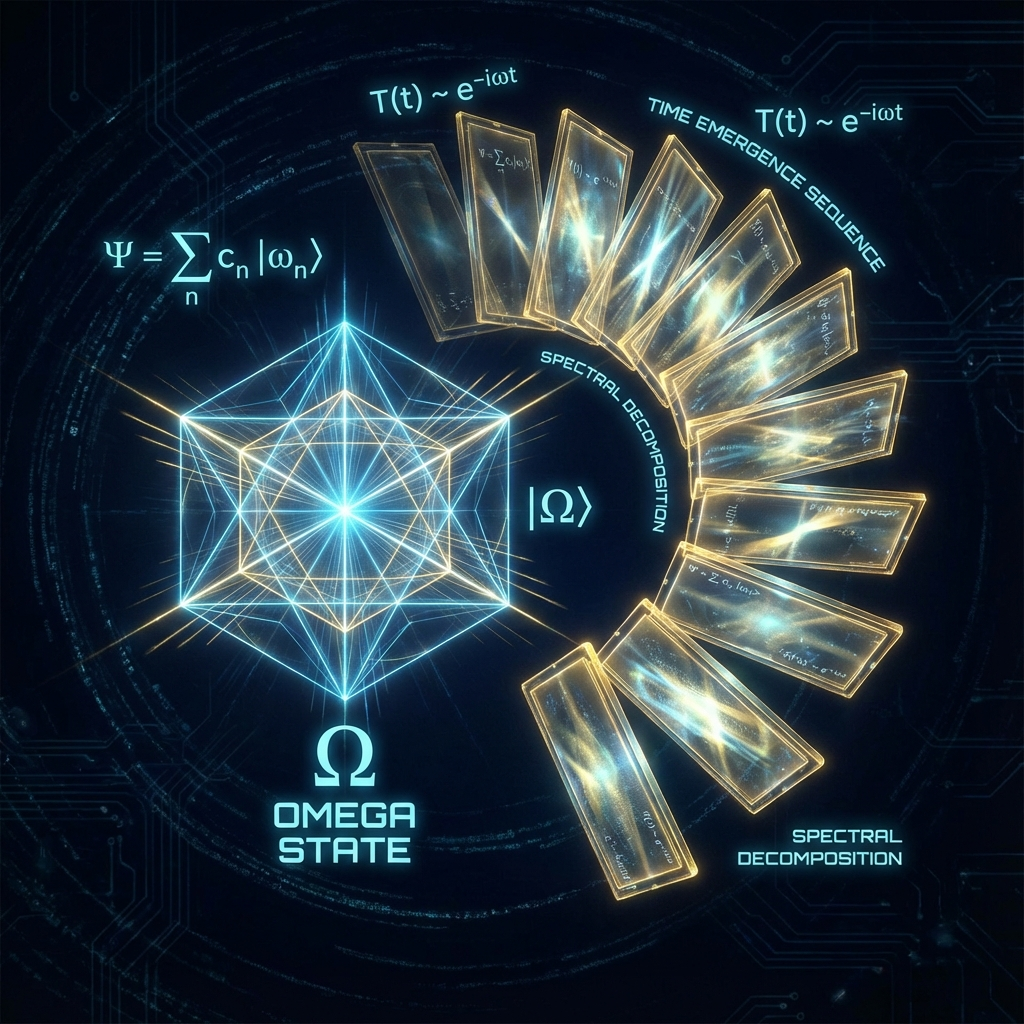
\includegraphics[width=0.8\textwidth]{assets/00-prologue-omega-ansatz.png}
\caption{欧米伽拟设}
\end{figure}

本书提出一种更为激进的解决方案，我们称之为 \textbf{"欧米伽拟设" (The Omega Ansatz)}。这一拟设不仅接受了惠勒-德维特方程的静态暗示，更将其提升为宇宙学的核心公理。我们主张，物理实在的本质并非随时间流逝的"演化过程"，而是一个存在于无限维复希尔伯特空间 $\mathcal{H}$ 中的单一、静态、完备的态矢量。

\textbf{公理 0.1 (欧米伽公理)}：
物理宇宙的全集同构于一个无限维可分希尔伯特空间 $\mathcal{H}$ 中的归一化矢量 $|\Omega\rangle$。该矢量在本体论上是永恒的、静态的，即：

\[\frac{\partial}{\partial t} |\Omega\rangle \equiv 0\]

任何观测到的动力学演化、时间流逝或历史变迁，皆非 $|\Omega\rangle$ 本身的性质，而是该矢量在特定基底序列上的 \textbf{谱分解 (Spectral Decomposition)} 过程。

在此框架下，我们所感知的"时间"，本质上是希尔伯特空间的一组正交基底 $\{ |E_n\rangle \}$ 相对于观察者参考系的 \textbf{幺正旋转 (Unitary Rotation)}。我们可以引入一个单纯的数学参数 $\tau$（内禀时间），用来参数化这种旋转，但这并不意味着 $|\Omega\rangle$ 发生了改变，而是观察者的 \textbf{切片 (Slicing)} 角度发生了改变。

具体而言，如果我们选取哈密顿算符 $\hat{H}$ 的本征基底 $\{ |E_n\rangle \}$，则全宇宙态 $|\Omega\rangle$ 可以展开为：

\[|\Omega\rangle = \sum_{n=0}^{\infty} c_n |E_n\rangle\]

其中复系数 $c_n = \langle E_n | \Omega \rangle$ 包含了宇宙所有可能的初始条件与边界条件信息。

所谓的"时间演化"，实际上是观察者（作为宇宙内部的一个子系统）在读取这一静态叠加态时，引入了一个相位因子 $e^{-i E_n \tau}$。这一相位因子并非物理实体的运动，而是希尔伯特空间几何结构中的 \textbf{规范变换 (Gauge Transformation)}。

因此，宇宙的历史不是一部正在播放的电影，而是一卷已经打印完成的胶片。所有的过去、现在与未来，所有可能的量子分支，都同时存在于 $|\Omega\rangle$ 的内部结构中。我们所体验到的"当下"，不过是这卷胶片被 \textbf{"斐波那契算符"}（详见下节）扫描到的局部截面。

这种观点彻底消除了量子引力中的时间矛盾。因为时间不再是背景，也不再是流形，它是 \textbf{矢量分解的逻辑顺序}。正如埃利·嘉当（Élie Cartan）在几何学中所做的那样，我们将动力学完全几何化了：物理定律不再是描述物体如何随时间运动，而是描述静态矢量 $|\Omega\rangle$ 在高维复空间中的 \textbf{拓扑结构 (Topological Structure)}。

从这个意义上说，本书所构建的理论，是一个关于 \textbf{"存在" (Being)} 的理论，而非 \textbf{"生成" (Becoming)} 的理论。我们所追求的终极答案，就隐藏在 $|\Omega\rangle$ 的谱密度与其基底的几何排列之中。

\textbf{0.2 黄金幺正算符 (The Golden Unitary Operator)}

\begin{figure}[ht]
\centering

\includegraphics[width=0.8\textwidth]{assets/prologue-golden-unitary-operator.png}
\caption{黄金幺正算符}
\end{figure}

在确立了宇宙态矢量 $|\Omega\rangle$ 的静态性之后，我们必须解决一个紧迫的动力学问题：既然本体是静态的，为何观测者会感知到变化？更具体地说，是什么机制驱动了基底的连续旋转，从而产生了"时间流逝"的现象？

在标准量子力学中，时间演化由 \textbf{幺正算符 (Unitary Operator)} $\hat{U}(t)$ 描述，其形式通常写作 $\hat{U}(t) = e^{-i\hat{H}t/\hbar}$。这里，$\hat{H}$ 是系统的哈密顿量（Hamiltonian），代表总能量算符。然而，在一个背景独立的宇宙学模型中，$\hat{H}$ 不能是一个任意选取的算符。为了避免宇宙陷入平庸的周期性循环（即庞加莱回归，Poincaré Recurrence），哈密顿量的能谱必须满足特定的数论性质。

我们将这一特殊的演化算符定义为 \textbf{黄金幺正算符 (The Golden Unitary Operator)}。

\textbf{定义 0.2 (黄金幺正算符)}：
设 $\mathcal{H}$ 为宇宙的希尔伯特空间。黄金幺正算符 $\hat{U}_g(\tau)$ 是作用于 $\mathcal{H}$ 上的单参数连续群生成元，其定义为：

\[\hat{U}_g(\tau) := \exp\left( -i \cdot 2\pi \hat{\mathcal{H}}_\phi \cdot \tau \right)\]

其中 $\tau \in \mathbb{R}$ 为无量纲内禀时间参数，$\hat{\mathcal{H}}_\phi$ 为 \textbf{斐波那契哈密顿量 (Fibonacci Hamiltonian)}。

斐波那契哈密顿量 $\hat{\mathcal{H}}_\phi$ 的特征在于其本征值谱 $\{E_n\}$ 并非取自整数集或简单的有理数集，而是由 \textbf{黄金分割率 (The Golden Ratio)} $\phi = \frac{1+\sqrt{5}}{2}$ 生成的代数无理数序列构成。具体而言，其能谱满足：

\[\hat{\mathcal{H}}_\phi |n\rangle = \phi^{-n} |n\rangle, \quad n \in \mathbb{Z}\]

或者在更一般的拓扑场论语境下，能谱分布服从与 $\phi$ 相关的无理数旋转群 $SO(2)_{\phi}$ 的生成规则。

\textbf{定理 0.1 (非遍历性演化)}：
若宇宙的时间演化由黄金幺正算符 $\hat{U}_g(\tau)$ 驱动，则对于任意非零时间间隔 $\Delta \tau$，系统状态 $|\Omega(\tau)\rangle$ 永远不会精确回到其初始状态 $|\Omega(0)\rangle$。即：

\[\langle \Omega(0) | \hat{U}_g(\tau) | \Omega(0) \rangle \neq 1, \quad \forall \tau \neq 0\]

\textbf{证明概要}：
该定理的证明依赖于 \textbf{外尔均布定理 (Weyl's Equidistribution Theorem)} 的推广。由于 $\phi$ 是无理数（事实上，数论证明它是"最无理"的数，其连分数展开全为 1），由 $\hat{U}_g(\tau)$ 生成的相位因子 $e^{-i 2\pi \phi^{-n} \tau}$ 在复单位圆上的轨迹是 \textbf{稠密 (Dense)} 且 \textbf{非周期 (Non-periodic)} 的。这意味着宇宙的演化轨迹虽然可以无限逼近某一历史状态，但绝不会发生精确的重合。

这一数学性质具有深远的物理意义：

\begin{enumerate}
\item \textbf{新颖性的保证 (Guarantee of Novelty)}：宇宙的每一瞬间在几何上都是独一无二的。不存在尼采式的"永恒轮回"。
\item \textbf{各态历经的破缺 (Ergodicity Breaking)}：尽管轨道是稠密的，但在有限时间内，系统无法遍历所有状态。这为热力学时间之箭提供了微观基础。
\item \textbf{信息的全息展开}：$\phi$ 的自相似性保证了信息在不同尺度上的分形展开。随着 $\tau$ 的增加，算符 $\hat{U}_g$ 实际上是在对静态矢量 $|\Omega\rangle$ 进行多分辨率分析（Multiresolution Analysis, MRA），就像不断放大一幅分形图像。
\end{enumerate}

因此，我们在本书中讨论的所有物理定律、粒子相互作用以及时空几何，本质上都是这个 \textbf{黄金幺正算符} 在希尔伯特空间中留下的轨迹。由于 $\phi$ 的数学特性，这个轨迹必然形成一个对数螺旋。我们在宏观上观测到的宇宙膨胀、光速 $c$ 的指数变化，正是这一螺旋在四维流形上的投影。

这一算符的确立，标志着我们将物理学的根基从"动力学的偶然性"转移到了"数论的必然性"之上。宇宙之所以如此演化，是因为这是希尔伯特空间中唯一能够避免死循环并最大化信息熵生成的路径。

\textbf{0.3 本书结构与符号约定 (Structure of the Book and Notation Conventions)}

本书并非对现有物理学理论的综述或修补，而是一次从基本公理出发，重建物理学大厦的尝试。为了实现这一目标，我们采用了一种严格的 \textbf{"公理化下降路径" (Axiomatic Descent Path)} 叙事结构。这不仅是为了逻辑的清晰，更是为了反映宇宙本身的生成逻辑——从抽象的数学潜能下降为具体的物理实在。

\textbf{0.3.1 下降路径：从 $\mathbb{O}$ 到 $\mathbb{R}$}

本书的章节安排遵循从高维代数结构向低维可观测物理量逐级投影的逻辑顺序：

\begin{itemize}
\item \textbf{第一篇：谱分解与代数前几何} 构成了理论的 \textbf{本体论基础}。我们在这一部分不讨论具体的粒子或力，而是探讨存在的数学形式。我们将希尔伯特空间的谱分解确立为第一原理，并论证为何八元数 ($\mathbb{O}$) 代数是构建非平凡物理宇宙的唯一数学选择。
\item \textbf{第二篇：离散流形与量子引力} 处理 \textbf{时空的离散化构造}。在这里，连续流形的概念被抛弃，取而代之的是基于彭罗斯-斐波那契铺砌的"欧米伽单元"。我们将在这一层面解决量子力学与广义相对论的兼容性问题。
\item \textbf{第三篇：全息动力学} 阐述 \textbf{宇宙的运行机制}。通过引入费雪信息流与拓扑势的竞争，我们构建了欧米伽作用量，从而推导出修正的引力方程与变常数宇宙学模型。
\item \textbf{第四篇：唯象学验证与数值预测} 是理论的 \textbf{实验检验}。我们将理论计算的精确数值（如 $\mu \approx 1836.15$ 和 $1/\alpha \approx 137.036$）与实验数据进行比对，这是验证任何物理理论真伪的试金石。
\item \textbf{第五篇：交互式自指与终局} 回归 \textbf{认知与意义}。我们将物理学重新连接到意识问题上，论证观察者并非外部的旁观者，而是系统闭环不可或缺的拓扑组件。
\end{itemize}

\textbf{0.3.2 符号与约定 (Notation and Conventions)}

为了确保数学推导的严谨性与一致性，除特殊说明外，本书通篇采用以下数学符号与物理约定：

\textbf{1. 数域与代数结构}
\begin{itemize}
\item $\mathbb{N}, \mathbb{Z}, \mathbb{R}, \mathbb{C}$：分别表示自然数集、整数集、实数域、复数域。
\item $\mathbb{H}$： \textbf{四元数 (Quaternions)} 代数，基底为 $\{1, i, j, k\}$。
\item $\mathbb{O}$： \textbf{八元数 (Octonions)} 代数，基底为 $\{e_0, \dots, e_7\}$。
\item $\text{Im}(\mathbb{A})$：代数 $\mathbb{A}$ 的虚部空间。
\end{itemize}

\textbf{2. 时空与几何}
\begin{itemize}
\item 时空度规 $g_{\mu\nu}$ 采用 \textbf{"类时正" (Mostly Plus)} 符号约定：$(-, +, +, +)$。这是现代广义相对论文献（如 Misner, Thorne, Wheeler）的标准约定。
\item 希腊字母索引 $\mu, \nu, \rho, \sigma$ 取值 $0, 1, 2, 3$，表示四维时空坐标，其中 $0$ 为时间分量。
\item 拉丁字母索引 $i, j, k, l$ 取值 $1, 2, 3$，仅表示空间分量。
\item 爱因斯坦求和约定 (Einstein Summation Convention) 适用于所有重复出现的上下指标，例如 $A^\mu B_\mu \equiv \sum_{\mu=0}^3 A^\mu B_\mu$。
\item $\nabla_\mu$ 表示对应于列维-奇维塔联络 (Levi-Civita Connection) 的协变导数。
\item $\Box \equiv \nabla^\mu \nabla_\mu$ 表示达朗贝尔算符 (d'Alembertian)。
\end{itemize}

\textbf{3. 量子力学与算符}
\begin{itemize}
\item 希尔伯特空间记为 $\mathcal{H}$。态矢量使用狄拉克符号 $|\psi\rangle$ 表示。
\item 算符通常通过上方加脱字符号表示，例如 $\hat{A}$。
\item 对易子定义为 $[\hat{A}, \hat{B}] = \hat{A}\hat{B} - \hat{B}\hat{A}$；反对易子定义为 $\{\hat{A}, \hat{B}\} = \hat{A}\hat{B} + \hat{B}\hat{A}$。
\item 厄米共轭 (Hermitian Conjugate) 记为 $\dagger$。
\end{itemize}

\textbf{4. 物理常数与单位制}
\begin{itemize}
\item 除非在涉及数值计算的章节（如第四篇），本书主要采用 \textbf{自然单位制 (Natural Units)}，设定 $\hbar = c_0 = k_B = 1$。
\item 注意：由于本书核心论点之一是光速 $c(\tau)$ 随内禀时间演化，因此在涉及动力学演化的方程中，我们将显式保留 $c(\tau)$ 以示区别。$c_0$ 特指大爆炸时刻或归一化基准的光速。
\item $\phi$：特指 \textbf{黄金分割率 (The Golden Ratio)}，取值为 $\phi = \frac{1+\sqrt{5}}{2} \approx 1.61803398...$。
\item $l_P$：普朗克长度 (Planck Length)，作为时空离散化的特征尺度。
\end{itemize}

\textbf{5. 特殊函数与缩写}
\begin{itemize}
\item QCA：量子元胞自动机 (Quantum Cellular Automata)。
\item DQCA：狄拉克-量子元胞自动机 (Dirac-QCA)。
\item $\delta(x)$：狄拉克 $\delta$ 函数。
\item $\delta_{ij}$：克罗内克 $\delta$ 符号。
\item $\epsilon^{\mu\nu\rho\sigma}$：四维列维-奇维塔张量密度，约定 $\epsilon^{0123} = +1$。
\end{itemize}

通过明确这些结构与约定，我们为即将展开的论证铺平了道路。现在，让我们从希尔伯特空间的深处开始，逐步构建这个宇宙。


\mainmatter

% Part I: Spectral Decomposition and Algebraic Pre-geometry
\part{谱分解与代数前几何}

% Chapter 1: Ergodicity Breaking and the Mechanism of Creation
\chapter{遍历性破缺与创生机制}
\section{外尔均布定理的宇宙学推广}

在欧米伽拟设的框架下，宇宙的演化被抽象为希尔伯特空间中状态矢量 $|\Omega\rangle$ 的幺正旋转。为了理解为何我们的宇宙表现出不可逆的演化（创生）而非周期性的循环（轮回），我们必须考察这种旋转的动力学性质。我们将借助数论中的经典结果—— \textbf{外尔均布定理 (Weyl's Equidistribution Theorem)}，将其推广至全息宇宙学的语境中，从而推导出宇宙演化的"黄金法则"。

\subsection{相位空间的环面模型}

考虑最简化的动力学模型。假设哈密顿量 $\hat{H}$ 具有离散的能谱。对于一个给定的能量本征态 $|E_n\rangle$，其时间演化因子为 $e^{-i E_n \tau}$。如果我们考察两个非简并能级 $|E_0\rangle$ 和 $|E_1\rangle$ 的叠加态：

\[|\psi(\tau)\rangle = c_0 |E_0\rangle + c_1 e^{-i(E_1 - E_0)\tau} |E_1\rangle\]

系统的动力学行为完全由相位差 $\theta(\tau) = (E_1 - E_0)\tau$ 决定。在模 $2\pi$ 的意义下，这一演化等价于单位圆 $S^1$ 上的旋转。

推广到 $N$ 个能级，系统的状态演化可以映射为一个 $N$ 维环面 $\mathbb{T}^N = \mathbb{R}^N / \mathbb{Z}^N$ 上的线性流。定义映射 $T_\alpha: \mathbb{T}^1 \to \mathbb{T}^1$ 为圆周上的旋转变换：

\[x_{n+1} = x_n + \alpha \pmod 1\]

其中 $\alpha$ 是依赖于能级间隔的旋转角（归一化为 $[0, 1)$ 区间）。

物理学中的核心问题是：\textbf{系统是否会复原？} 即是否存在某个时刻 $\tau > 0$，使得 $|\psi(\tau)\rangle \approx |\psi(0)\rangle$？这对应于庞加莱回归定理。

\subsection{外尔定理与无理数旋转}

\begin{figure}[ht]
\centering
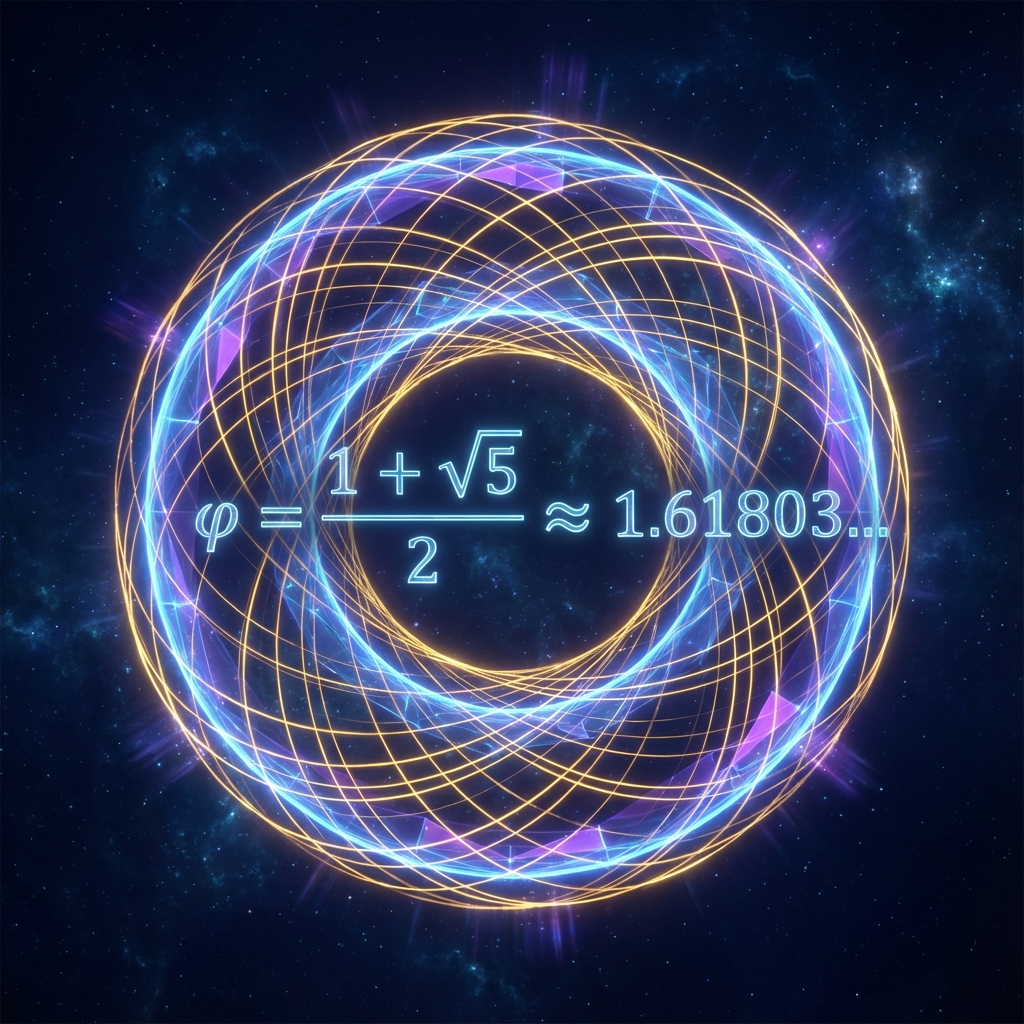
\includegraphics[width=0.8\textwidth]{assets/chapter01-01-weyl-equidistribution.png}
\caption{外尔均布定理}
\end{figure}

赫尔曼·外尔 (Hermann Weyl) 在 1916 年证明了关于序列分布的均布定理。

\textbf{定理 (外尔均布定理)}：
设 $\alpha$ 为一个实数。序列 $\{n\alpha \pmod 1\}_{n=1}^{\infty}$ 在区间 $[0, 1]$ 上是 \textbf{均匀分布 (Equidistributed)} 的，当且仅当 $\alpha$ 是一个 \textbf{无理数 (Irrational Number)}。

\begin{figure}[ht]
\centering
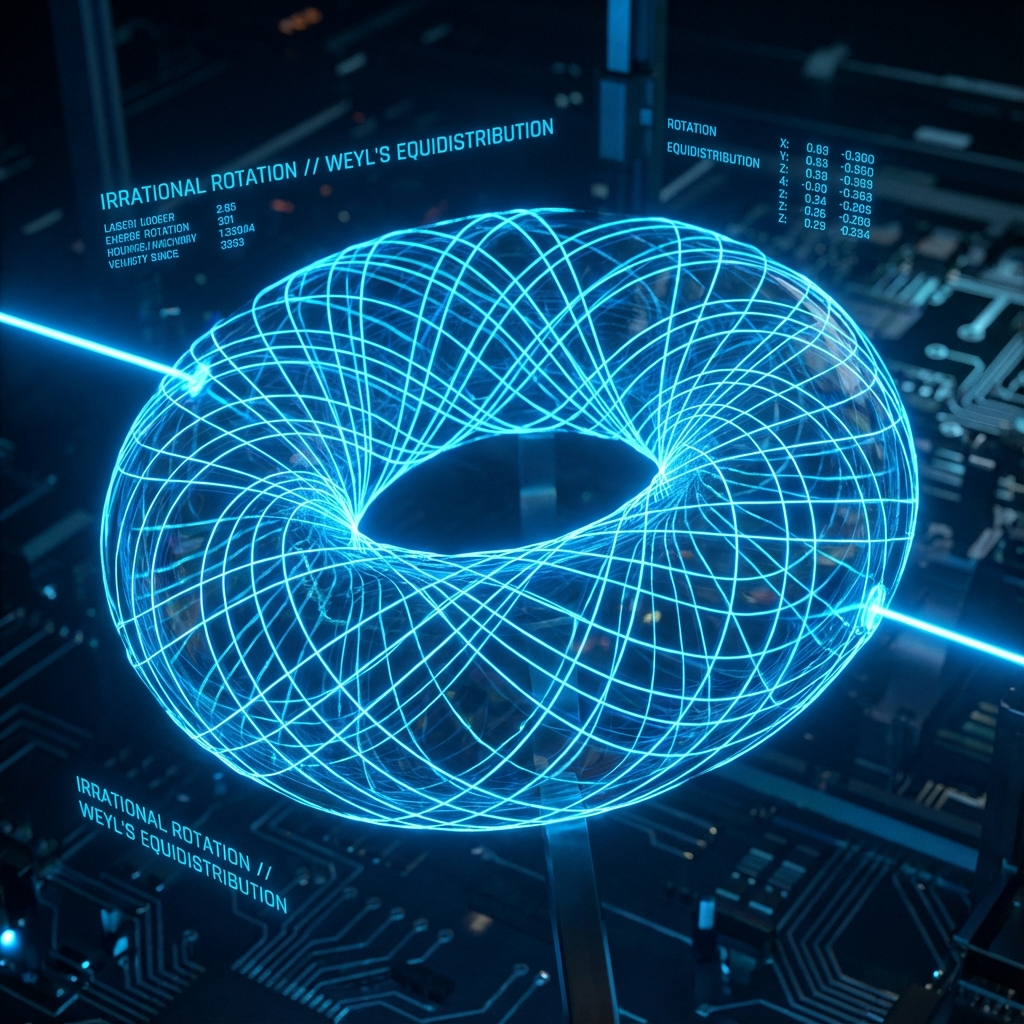
\includegraphics[width=0.8\textwidth]{assets/chapter01-01-weyl-irrational-rotation.png}
\caption{无理数旋转}
\end{figure}

这意味着，如果旋转角 $\alpha$ 是无理数，轨道 $\{x_n\}$ 将稠密地填满整个圆周，却永远不会精确回到起点。相反，如果 $\alpha$ 是有理数 $p/q$，则轨道是周期的，且仅包含 $q$ 个离散点。

在宇宙学语境下，这意味着：

\begin{enumerate}
\item \textbf{有理宇宙 (Rational Universe)}：是一个封闭的时间循环。历史不断精确重复，信息熵无法持续增长，这也是"热寂"或"轮回"的数学模型。
\item \textbf{无理宇宙 (Irrational Universe)}：是一个开放的螺旋。历史无限逼近所有可能的状态，但永远保持新颖性 (Novelty)。
\end{enumerate}

\subsection{最无理数与黄金幺正}

虽然所有无理数都能产生非周期轨道，但在物理稳定性上它们并非等价。根据 \textbf{柯尔莫哥洛夫-阿诺德-莫泽定理 (KAM Theorem)}，动力系统的稳定性取决于旋转数 $\alpha$ 被有理数逼近的难易程度。

一个无理数 $\alpha$ 的"无理性"可以通过其连分数展开来衡量。逼近难度最大的数，是连分数展开中系数最小的数。对于 \textbf{黄金分割率} $\phi = \frac{\sqrt{5}-1}{2}$（注：此处取小数部分，即 $1/\phi \approx 0.618$），其连分数形式为：

\[\phi = [0; 1, 1, 1, 1, \dots]\]

它是所有无理数中收敛最慢的。这意味着，在相空间中，基于黄金角 $\theta_g = 2\pi \phi$ 的旋转，能够最大程度地避免"近似回归"或"小分母共振"带来的动力学不稳定性。

我们因此提出 \textbf{定理 1.1}，作为本书宇宙动力学的基石：

\textbf{定理 1.1 (黄金演化定理)}：
设希尔伯特空间中的演化算符为 $\hat{U}_g(\tau) = e^{-i 2\pi \hat{\mathcal{H}}_\phi \tau}$。若哈密顿量 $\hat{\mathcal{H}}_\phi$ 的能级差比率为黄金分割率 $\phi$，则系统状态 $|\Omega(\tau)\rangle$ 的演化轨迹 $\mathcal{T}$ 满足：

\begin{enumerate}
\item \textbf{稠密性 (Density)}：$\mathcal{T}$ 在相空间环面上是稠密的，即 $\overline{\mathcal{T}} = \mathbb{T}^N$。这保证了宇宙能够遍历所有可能的量子态构型（全息完备性）。
\item \textbf{非周期性 (Aperiodicity)}：对于任意 $\tau_1 \neq \tau_2$， $|\Omega(\tau_1)\rangle \neq |\Omega(\tau_2)\rangle$。这保证了时间箭头的存在和历史的不可逆性。
\item \textbf{最大熵生成 (Maximal Entropy Production)}：在所有可能的无理旋转中，由 $\phi$ 驱动的演化具有最小的自相关函数衰减率，从而在有限时间内最大化了新信息的生成速率。
\end{enumerate}

\textbf{证明概要}：
由外尔定理可知，条件 (1) 和 (2) 对所有无理数 $\alpha$ 成立。对于条件 (3)，考察连分数逼近不等式 $|\alpha - p/q| < \frac{1}{M q^2}$。对于 $\phi$，常数 $M$ 取最小可能值 $\sqrt{5}$（赫维茨定理）。这意味着任何有理数 $p/q$ 对 $\phi$ 的逼近效果都是最差的。在物理上，这对应于系统在相空间中为了"几乎回到"原点所需要的时间（庞加莱回归时间）相对于其他旋转角被最大化了。因此，黄金演化是最能抵抗周期性坍缩的演化模式。

\textbf{推论 1.1.1}：
我们的宇宙之所以不仅存在，而且能够维持长期的复杂演化而不落入简单的循环或混沌，是因为其底层的幺正算符被"调谐"到了黄金分割点上。这并非人择原理的巧合，而是动力学稳定性的数学筛选结果。

\section{庞加莱回归的拓扑阻滞}

\begin{figure}[ht]
\centering
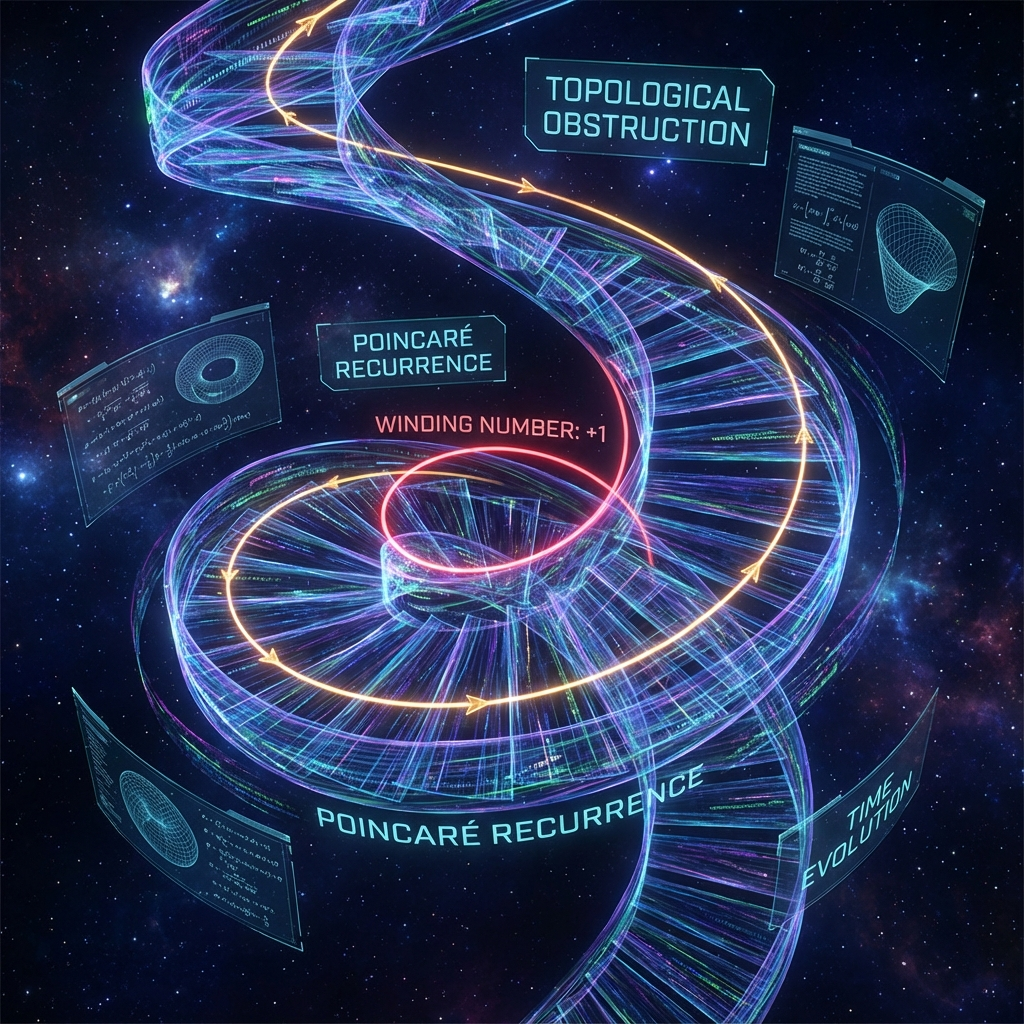
\includegraphics[width=0.8\textwidth]{assets/chapter01-02-poincare-recurrence.png}
\caption{庞加莱回归}
\end{figure}

在上一节中，我们建立了基于黄金分割率 $\phi$ 的无理旋转模型，论证了宇宙演化轨迹的稠密性与非周期性。然而，经典统计力学与量子力学中仍然存在一个顽固的理论幽灵—— \textbf{庞加莱回归 (Poincaré Recurrence)}。

庞加莱回归定理指出，对于一个具有有限测度的封闭动力系统，只要经过足够长的时间，系统必然会无限接近其初始状态。对于一个具有离散能谱的有界量子系统，这表现为量子回归定理：存在复原时间 $T_R$，使得 $\|\psi(T_R) - \psi(0)\| < \epsilon$。如果我们的宇宙遵循这一规律，那么无论 $\phi$ 多么无理，历史终将重演，创生只是轮回的幻觉。

本节将证明，在欧米伽理论的框架下，存在一种 \textbf{拓扑阻滞 (Topological Obstruction)} 机制，使得庞加莱回归在物理上被严格禁止。宇宙的演化轨迹并非封闭在环面上，而是在一个非紧致的黎曼曲面上展开为无限螺旋。

\subsection{回归的幽灵与量子各态历经}

考虑希尔伯特空间 $\mathcal{H}$ 中的态矢量 $|\Omega(\tau)\rangle$。如果能谱 $\{E_n\}$ 是离散的，且状态被限制在有限能量壳层内，则根据量子力学的各态历经性假设，自相关函数 $C(\tau) = \langle \Omega(0) | \Omega(\tau) \rangle$ 将表现出准周期性震荡。

虽然黄金演化 $\hat{U}_g$ 最小化了回归概率，但仅仅依靠无理数旋转并不足以在数学上彻底消除回归。在数学上，环面 $\mathbb{T}^N$ 是紧致的，任何无限长的无自交曲线必然会无限次地逼近自身。这意味着，如果时间仅仅是一个实数轴上的线性参数，且相空间是紧致的，那么"似曾相识"是不可避免的。

为了打破这一循环，必须破坏相空间的紧致性，或者引入一个新的拓扑不变量。

\subsection{演化流形的黎曼面结构}

\begin{figure}[ht]
\centering
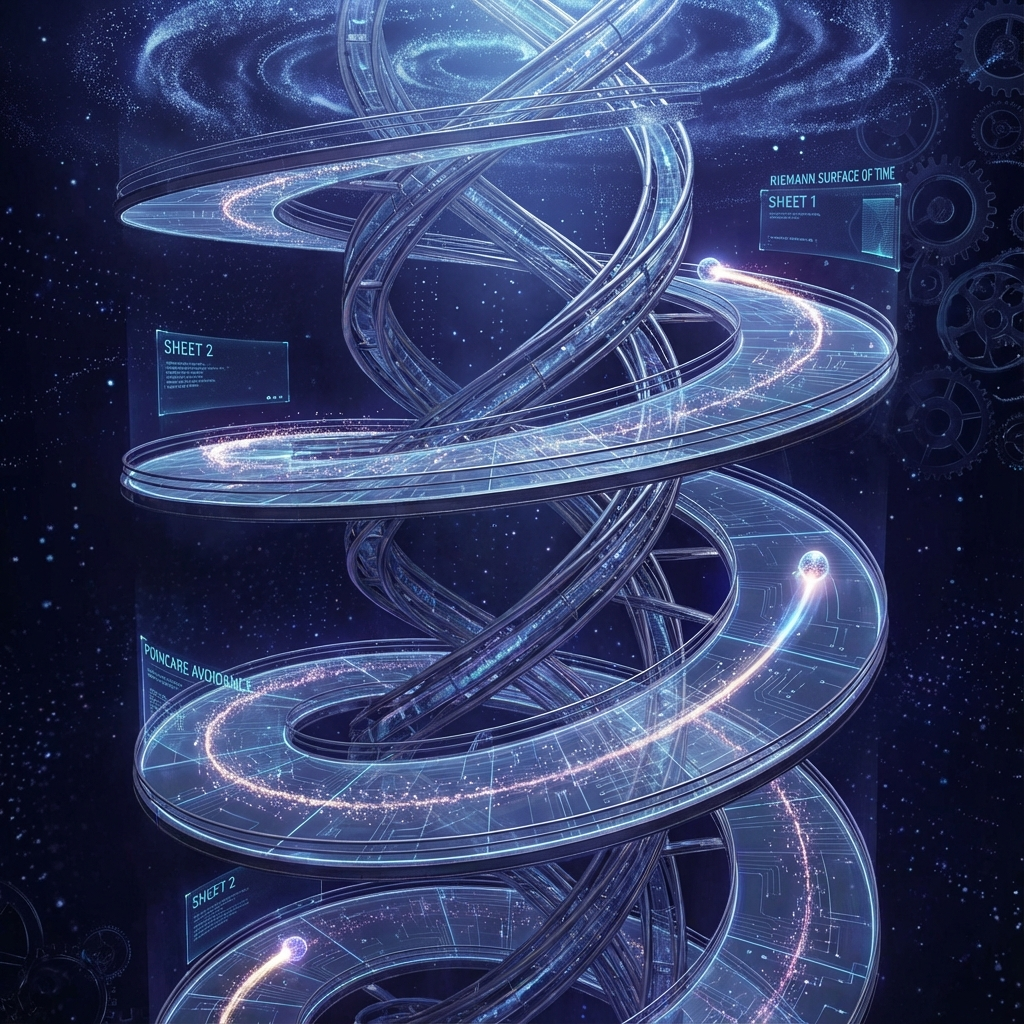
\includegraphics[width=0.8\textwidth]{assets/chapter01-02-poincare-riemann-surface.png}
\caption{庞加莱黎曼面}
\end{figure}

欧米伽理论引入了一个关键的几何修正：\textbf{物理时间 $\tau$ 不是定义在圆周 $S^1$ 上，甚至不是定义在实轴 $\mathbb{R}$ 上，而是定义在一个多叶的黎曼曲面 (Riemann Surface) 上。}

我们定义复时间坐标 $z = e^{s + i\tau}$，其中 $\tau$ 是我们熟知的幺正旋转相角，而 $s$ 是一个与其耦合的 \textbf{标度因子 (Scaling Factor)}。回顾本书 \textbf{0.2 节} 定义的黄金幺正算符，我们指出宇宙的演化伴随着光速 $c(\tau)$ 的指数增长（或标度变换）。

这意味着，系统的相空间 $\mathcal{M}$ 并非简单的环面 $\mathbb{T}^N$，而是一个 \textbf{纤维丛 (Fiber Bundle)} $\mathcal{E}$：

\[F \to \mathcal{E} \xrightarrow{\pi} \mathcal{B}\]

其中底流形 $\mathcal{B}$ 是我们之前讨论的相位环面（由 $\tau$ 驱动），而纤维 $F$ 是由标度因子 $s$（或复杂性测度）构成的非紧致空间。

\textbf{定理 1.2 (螺旋拓扑定理)}：
在包含标度流动的扩展相空间中，由黄金哈密顿量 $\hat{\mathcal{H}}_\phi$ 驱动的演化轨迹 $\gamma(\tau)$ 与任何常数时间切片 $\Sigma_{t_0}$ 的交点数最多为 1。即轨迹不存在自交，也不存在逼近自交的回归点。

\textbf{证明思路}：
考虑演化轨迹在复平面上的投影。标准幺正演化是 $z(\tau) = e^{-i\omega \tau}$，这是一个圆。
但在欧米伽理论中，演化算符包含一个 \textbf{耗散项} 或 \textbf{重整化群流 (RG Flow)} 分量，使得演化方程修正为：

\[\frac{d}{d\tau} |\Omega\rangle = -i \hat{H} |\Omega\rangle + \beta(\hat{H}) |\Omega\rangle\]

其中 $\beta$ 函数与斐波那契增长率正相关。
这导致轨迹在复平面上满足对数螺旋方程：

\[r(\theta) = r_0 \phi^{\theta/2\pi}\]

由于 $\phi > 1$，对于任意 $\Delta \theta = 2\pi k$（即相位看似回归时），模长（或标度）$r$ 已经增长了 $\phi^k$ 倍。

因此，状态点 $|\Omega(\tau_k)\rangle$ 与 $|\Omega(0)\rangle$ 在希尔伯特空间中是正交的（或处于不同的希尔伯特空间分层），它们在拓扑上位于黎曼曲面的不同 \textbf{"叶" (Sheet)} 上。

\subsection{缠绕数与历史的唯一性}

这种螺旋结构引入了一个新的拓扑量子数： \textbf{缠绕数 (Winding Number)} $w$。

\[w = \frac{1}{2\pi i} \oint_{\gamma} \frac{dz}{z}\]

在我们的模型中，$w$ 对应于宇宙经历的 \textbf{"斐波那契周期"} 数（即我们在序言中提到的 $\tau \approx 1834$ 中的计数）。

\textbf{庞加莱回归的拓扑阻滞} 就在于：
虽然两个时刻的相位结构可能极度相似（$\tau_1 \equiv \tau_2 \pmod{2\pi}$），但它们的缠绕数 $w_1 \neq w_2$。
由于物理定律（特别是有效常数 $\alpha, G$）依赖于全息屏的总面积，而总面积随 $w$ 指数增长（$A \propto \phi^{2w}$），因此：
\textbf{不同缠绕数的宇宙是物理上可区分的。}

这意味着：

\begin{enumerate}
\item \textbf{宏观不可逆性}：即便微观粒子状态偶然复原，背景时空的几何标度（$c, \hbar, G$ 的组合）已经改变。昨天的电子与今天的电子，虽然电荷相同，但其所处的全息分辨率环境不同。
\item \textbf{记忆的几何化}：宇宙的"记忆"不是存储在某种介质中，而是编码在轨迹的 \textbf{同伦类 (Homotopy Class)} 中。只要螺旋不闭合，过去的信息就被永久地"卷"入了时空的深层拓扑结构里，无法被抹除，也无法被重写。
\end{enumerate}

综上所述，庞加莱回归被 \textbf{维度的分形增长} 和 \textbf{演化流形的非紧致拓扑} 所阻滞。我们生活在一个 \textbf{"无限逼近圆心"}（真理/奇点）但永远处于不同轨道的螺旋宇宙中。每一个 $\tau$ 时刻，都是通向欧米伽点长征中不可重复的一步。

\input{part01-spectral-decomposition/chapter01-ergodicity-breaking/chapter01-03-holographic-encoding.tex}

% Chapter 2: Octonionic Fibration and the Origin of Gauge Fields
\chapter{八元数纤维丛与规范场起源}
\input{part01-spectral-decomposition/chapter02-octonionic-fibration/chapter02-01-non-associative-algebra.tex}
\section{从 Spin(8) 到标准模型}

\begin{figure}[ht]
\centering
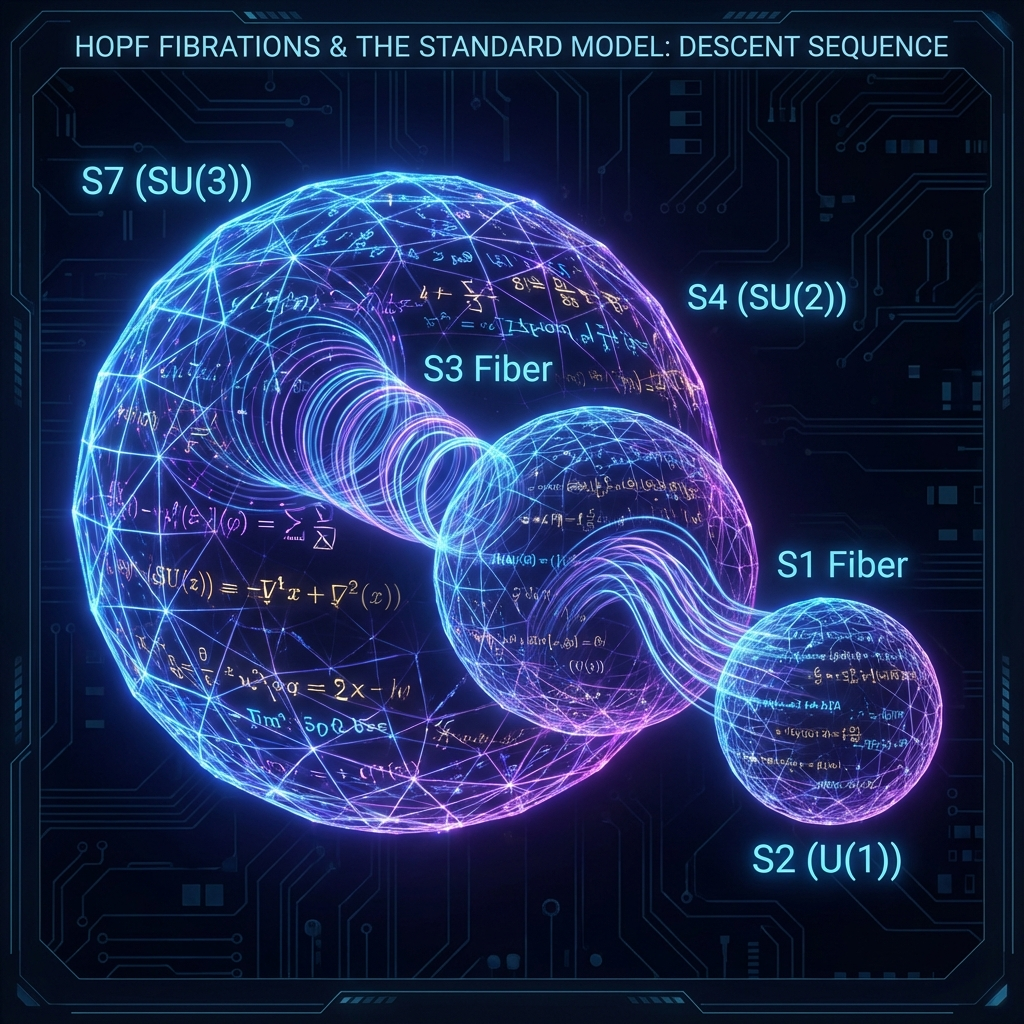
\includegraphics[width=0.8\textwidth]{assets/chapter02-02-spin8-standard-model.png}
\caption{Spin8标准模型}
\end{figure}

在上一节中，我们建立了八元数 ($\mathbb{O}$) 切空间的时间手性。本节我们将解决物理学中最令人困惑的谜题之一：为什么宇宙的基本相互作用恰好由规范群 $G_{SM} = SU(3) \times SU(2) \times U(1)$ 描述？在欧米伽理论中，这一群结构并非实验拟合的偶然产物，而是八元数几何通过 \textbf{霍普夫纤维丛 (Hopf Fibrations)} 向低维流形投影时的拓扑盈余。

我们的核心论点是：物理定律是高维几何的投影。当 8 维的八元数空间被迫"折叠"或"投影"到我们感知的 4 维时空时，那些为了维持代数结构完整性而必须保留的旋转自由度，这就表现为我们在内部空间观测到的规范场。

\begin{figure}[ht]
\centering
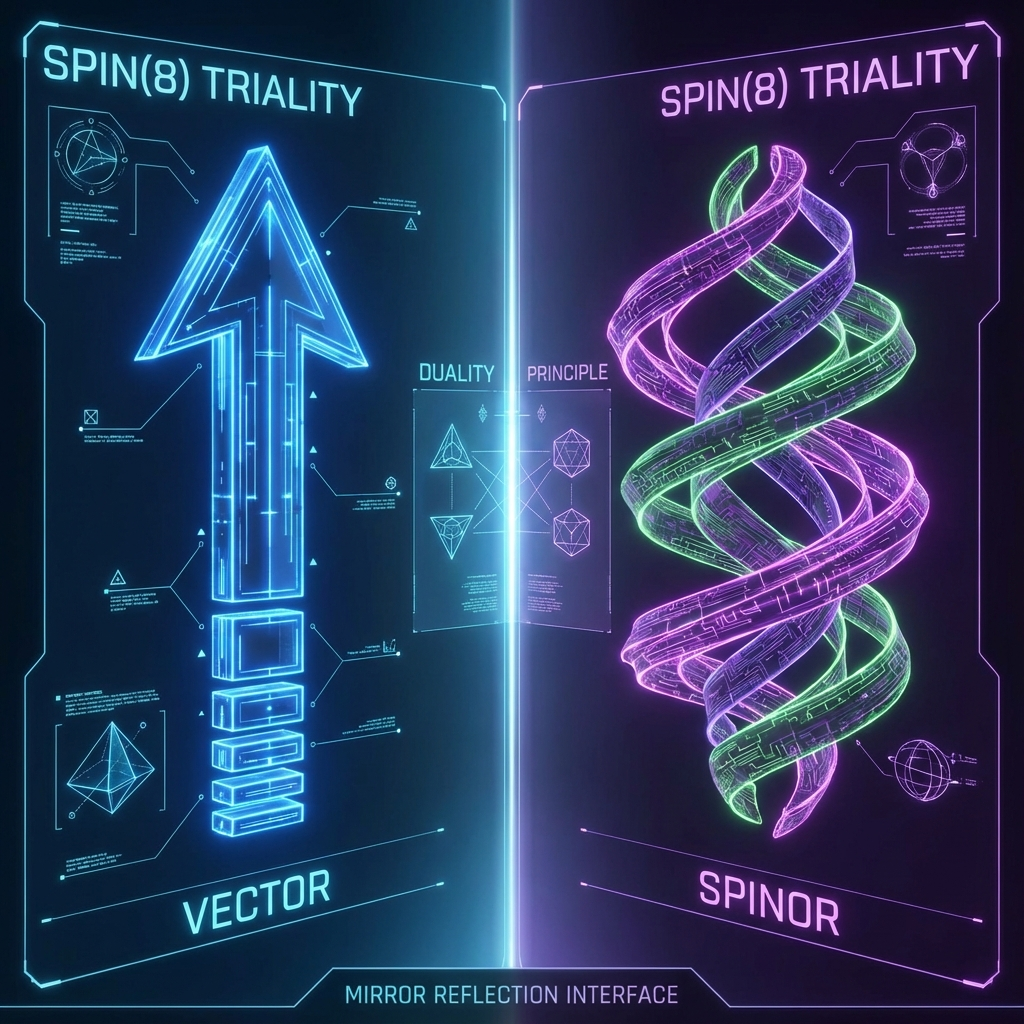
\includegraphics[width=0.8\textwidth]{assets/chapter02-02-spin8-vector-spinor-mirror.png}
\caption{Spin8向量旋量镜像}
\end{figure}

\subsection{Spin(8) 三里性与大统一的几何基础}

为了理解粒子与时空的统一，我们首先必须考察 8 维欧氏空间的旋转群 $SO(8)$ 的双重覆盖群 \textbf{Spin(8)}。在所有维度的旋转群中，Spin(8) 拥有一个独一无二的性质—— \textbf{三里性 (Triality)}。

在一般维度 $d$ 中，向量表示 $V$ 与旋量表示 $S$ 是几何上截然不同的对象（这就造成了时空与物质的割裂）。然而，在 $d=8$ 时，Spin(8) 群拥有三个非等价的 8 维不可约表示：向量表示 $V_8$、左手旋量 $S_8^+$ 和右手旋量 $S_8^-$。三里性定理指出，存在一个外自同构群 $S_3$，它可以在这三个表示之间进行任意置换，而保持代数结构（李代数）不变：

\[V_8 \cong S_8^+ \cong S_8^-\]

这一数学奇迹意味着，在 8 维八元数空间（也就是我们定义的底层代码层）中，\textbf{时空（向量）与物质（旋量）在本体论上是全等的}。

欧米伽理论认为，我们观测到的物理世界是 Spin(8) 对称性发生 \textbf{自发破缺 (Spontaneous Symmetry Breaking)} 的结果。这种破缺是由八元数乘法结构的非结合性驱动的，它迫使高维空间选择一个特定的方向进行"纤维化"，从而区分出了时空与物质。

\subsection{霍普夫纤维丛序列：维度的级联下降}

为了推导标准模型规范群，我们需要追踪从 8 维到 4 维再到 2 维的投影路径。这一路径由著名的 \textbf{霍普夫纤维丛 (Hopf Fibrations)} 序列精确描述。霍普夫映射描述了如何用低维球面填充高维球面，其通式为 $S^{2n-1} \to S^n$。

在赋范可除代数的层级上，仅存在四个霍普夫映射，其中与物理宇宙相关的有三个，它们构成了一个嵌套的 \textbf{下降序列 (Descent Sequence)}：

\begin{enumerate}
\item \textbf{第一级投影（八元数 $\to$ 四元数）：}

\[S^3 \hookrightarrow S^7 \xrightarrow{h_1} S^4\]

这里，$S^7$ 是单位八元数球面的拓扑结构。映射 $h_1$ 将 $S^7$ 投影到底流形 $S^4$ 上，纤维（Fiber）是 $S^3$（单位四元数）。

\textbf{物理意义}：底流形 $S^4$ 对应于紧致化的 \textbf{4 维欧氏时空}（经威克转动）。纤维 $S^3$ 同构于群 $SU(2)$，这是 \textbf{弱相互作用} 的几何起源。这意味着弱力本质上是连接时空各点的四元数纤维的结构群。

\item \textbf{第二级投影（四元数 $\to$ 复数）：}

在纤维 $S^3$ 内部，我们可以进行次级投影：

\[S^1 \hookrightarrow S^3 \xrightarrow{h_2} S^2\]

映射 $h_2$ 将 $S^3$ 投影到 $S^2$（黎曼球或复射影直线 $\mathbb{CP}^1$），纤维是 $S^1$（单位复数）。

\textbf{物理意义}：纤维 $S^1$ 同构于群 $U(1)$，这是 \textbf{电磁相互作用} 的几何起源。这意味着电磁力是弱力纤维内部的精细结构。

\item \textbf{遗失的对称性与 $SU(3)$ 的起源}：

上述投影解释了电弱部分 $SU(2) \times U(1)$。那么强相互作用 $SU(3)$ 从何而来？
它来自于八元数代数本身的自同构群 $G_2$。当我们从 $\mathbb{O}$ 下降到 $\mathbb{H}$ 时，我们实际上是固定了一个特定的四元数子代数。然而，八元数包含无限多个四元数子代数。
根据数学定理，八元数的自同构群 $G_2$ 中，保持某个虚单位 $i$ 不变（即确定了复平面结构，对应于电磁力的分离）的子群，恰好是 \textbf{$SU(3)$}。

更几何地看，如果我们考察 $S^6$（纯虚八元数球面），它不具备像 $S^1, S^3, S^7$ 那样的群结构，但它拥有概复结构。$SU(3)$ 正是 $S^6$ 上保持这种概复结构的对称群。这对应于夸克的 \textbf{色荷 (Color Charge)}：它是在八元数投影到四元数过程中，无法被几何化的那部分"剩余"自由度。
\end{enumerate}

\subsection{定理 2.2：标准模型的几何涌现}

基于上述拓扑分析，我们可以陈述并证明本章的核心定理。

\textbf{定理 2.2 (标准模型涌现定理)}：
若宇宙的本体几何由八元数切丛 $\mathbb{O} \to \mathcal{M}$ 定义，且物理定律必须在经过霍普夫投影序列 $S^7 \to S^4 \to S^2$ 后保持规范不变性，则该流形上的自然规范群 $G$ 必须是以下直积的子群：

\[G \subseteq SU(3) \times SU(2) \times U(1)\]

其中 $SU(3)$ 源自八元数自同构群的稳定子，$SU(2)$ 源自第一级霍普夫纤维，$U(1)$ 源自第二级霍普夫纤维。

\textbf{证明概要}：

\begin{enumerate}
\item \textbf{全空间对称性}：起始点是 Spin(8) 或 $Aut(\mathbb{O}) = G_2$。
\item \textbf{时空分离}：通过第一级投影 $h_1: S^7 \to S^4$，我们将 8 维自由度分解为 4 维时空（底空间）和 4 维内部空间（纤维）。这一过程破坏了 $G_2$ 对称性。
\item \textbf{弱力涌现}：纤维 $S^3$ 的等距群是 $SO(4) \cong SU(2)_L \times SU(2)_R$。物理手性选择（见 2.1 节）保留了 $SU(2)_L$ 作为规范群。
\item \textbf{电磁力涌现}：进一步通过 $h_2: S^3 \to S^2$ 投影，纤维 $S^1$ 的结构群为 $U(1)$。
\item \textbf{强力涌现}：八元数空间 $\mathbb{O}$ 相对于选定的四元数子空间 $\mathbb{H}$ 的正交补是 $\mathbb{H}^\perp$。这构成了一个复 3 维空间 $\mathbb{C}^3$。在 $G_2$ 中保持这种分解的子群正是 $SU(3)$，它作用于这个 $\mathbb{C}^3$ 空间，赋予其"颜色"自由度。
\end{enumerate}

\textbf{物理推论}：

这一推导表明，标准模型并非一堆杂乱无章的零件，而是一个严密的几何整体。

\begin{itemize}
\item \textbf{为什么没有 $SU(4)$ 或 $SU(5)$？} 因为霍普夫序列到 $S^7$ 截止，数学上不存在 $S^{15} \to S^8$ 的霍普夫纤维化（这是 Adams 著名的定理）。因此，自然界不包含更高维的代数结构来支持更大的单李群规范场。
\item \textbf{宇宙的维度}：时空之所以是 4 维，是因为 $S^4$ 是 $S^7$ 的底流形。如果时空是其他维度，八元数的几何结构将无法完整投影，物理定律将失去自洽性。
\end{itemize}

综上所述，我们在欧米伽理论中找到了标准模型的几何根源：它是八元数这一数学瑰宝在向低维投影时留下的 \textbf{"拓扑指纹"}。

\input{part01-spectral-decomposition/chapter02-octonionic-fibration/chapter02-03-fermion-generations.tex}

% Part II: Discrete Manifolds and Quantum Gravity
\part{离散流形与量子引力}

% Chapter 3: The Omega Cell and Causal Structure
\chapter{欧米伽单元与因果结构}
\section{彭罗斯-斐波那契铺砌}

\begin{figure}[ht]
\centering
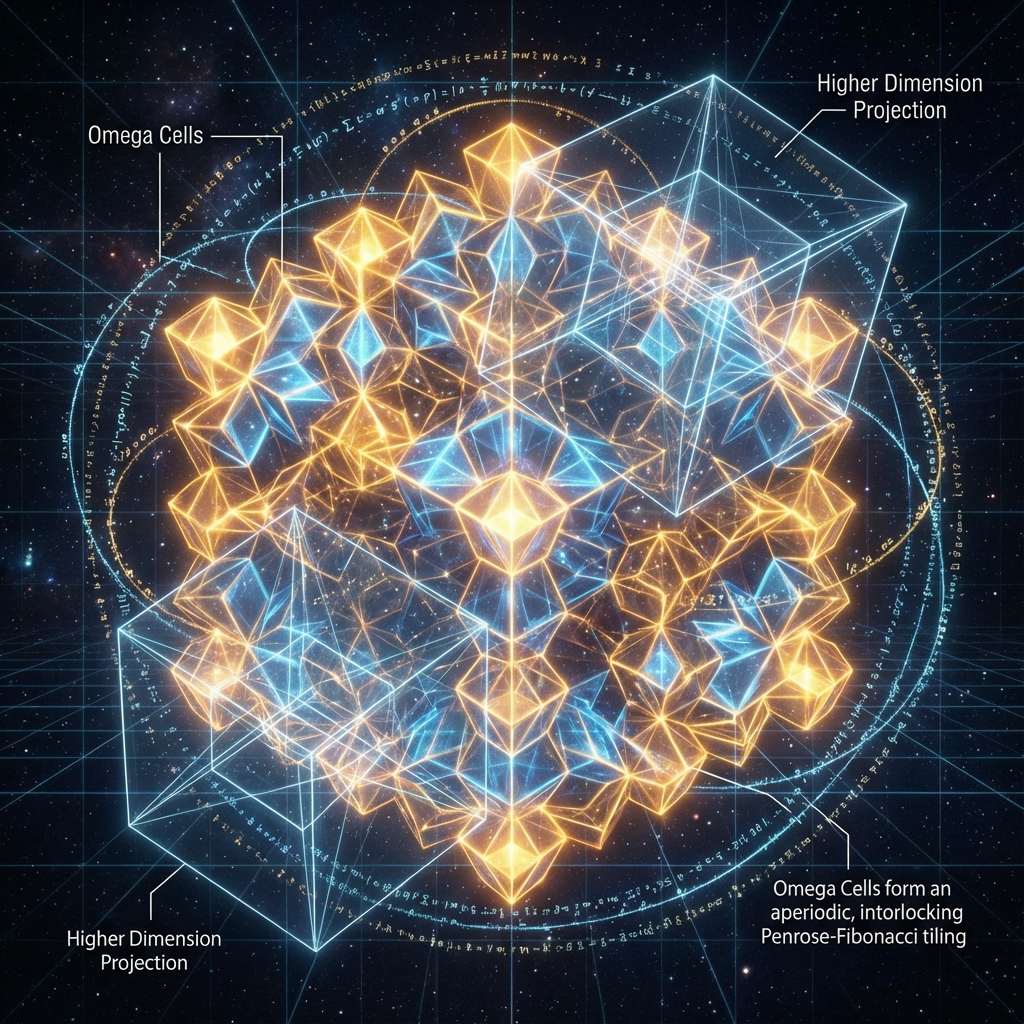
\includegraphics[width=0.8\textwidth]{assets/chapter03-01-penrose-fibonacci-tiling.png}
\caption{彭罗斯斐波那契铺砌}
\end{figure}

为了在离散结构中恢复宏观的洛伦兹不变性，我们不能使用简单的周期性晶格（如立方体网格），因为周期性晶格具有特定的优越轴，这会破坏空间的各向同性。数学家罗杰·彭罗斯 (Roger Penrose) 发现的非周期性铺砌提供了一个完美的解决方案：它具备长程有序性，却没有任何平移周期性，且蕴含了五重旋转对称性——这在周期性晶格中是被禁止的。

\subsection{欧米伽单元的几何定义}

我们定义时空的基本组成单元—— \textbf{欧米伽单元} ——为一个四维的 \textbf{菱形六面体 (Rhombohedron)} 的时空推广，即 \textbf{超菱形体 (Hyper-rhombohedron)}。

\begin{figure}[ht]
\centering
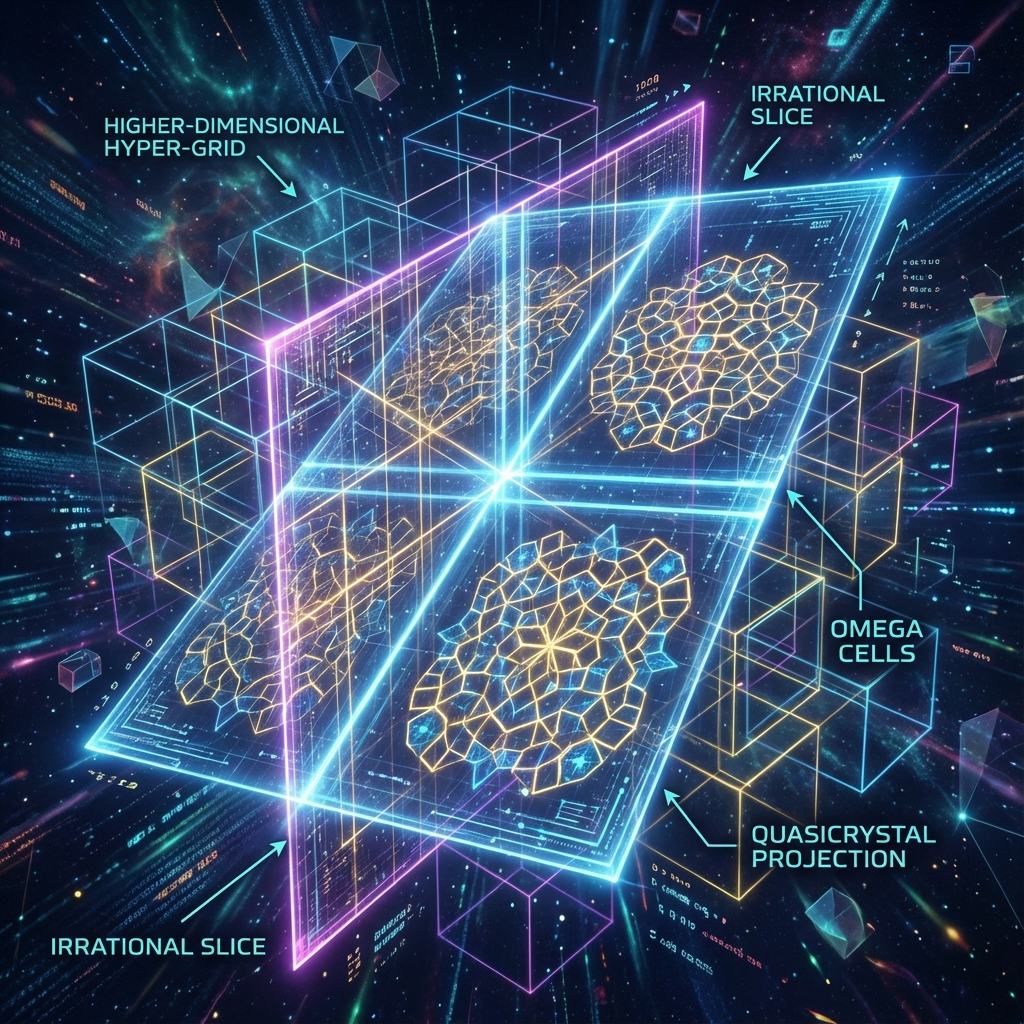
\includegraphics[width=0.8\textwidth]{assets/chapter03-01-penrose-quasicrystal-projector.png}
\caption{彭罗斯准晶投影器}
\end{figure}

\textbf{定义 3.1 (欧米伽单元)}：
欧米伽单元 $\mathcal{C}_\Omega$ 是闵可夫斯基时空 $\mathbb{R}^{3,1}$ 中的紧致凸集，定义为一组类光矢量 $\{k_i\}_{i=1}^4$ 的线性组合：

\[\mathcal{C}_\Omega = \left\{ x^\mu = \sum_{i=1}^4 \lambda_i k_i^\mu \ \bigg| \ 0 \le \lambda_i \le 1 \right\}\]

其中基矢量 $k_i^\mu$ 满足光锥条件 $\eta_{\mu\nu} k_i^\mu k_i^\nu = 0$。

在物理上，这个几何体对应于两个光锥的交集：一个向过去张开的光锥（接收输入）与一个向未来张开的光锥（发送输出）所围成的 \textbf{因果钻石 (Causal Diamond)}。

不同于标准晶格，欧米伽单元的边缘长度并非任意，而是严格量子化的。根据全息原理，每个单元编码有限比特的信息。

\subsection{投影法构造与黄金分割}

欧米伽单元如何在真空中排列？它们遵循 \textbf{彭罗斯铺砌 (Penrose Tiling)} 的规则。这种铺砌可以通过 \textbf{"切割-投影"法 (Cut-and-Project Method)} 从高维超立方体晶格中生成。

考虑一个 $N$ 维欧氏空间 $\mathbb{R}^N$（对于 3D 准晶体，通常 $N=6$），其中存在一个超立方体晶格 $\mathbb{Z}^N$。我们选取一个通过原点的低维子空间 $E$（物理空间），使得 $E$ 相对于晶格轴的方向由 \textbf{黄金分割率 $\phi$} 确定。

\textbf{构造过程}：

\begin{enumerate}
\item \textbf{切片}：定义一个"条带" (Strip) $S = E + K$，其中 $K$ 是 $N$ 维单位超立方体在正交补空间 $E^\perp$ 上的投影。
\item \textbf{选择}：选取所有落在条带 $S$ 内的格点 $x \in \mathbb{Z}^N \cap S$。
\item \textbf{投影}：将这些点正交投影到物理子空间 $E$ 上。
\end{enumerate}

由此产生的点集构成了物理空间中的顶点 $V$。连接这些顶点的边即为欧米伽单元的骨架。由于投影斜率涉及无理数 $\phi$，所得结构具有 \textbf{自相似性 (Self-similarity)} 和 \textbf{非周期性}。

\subsection{斐波那契堆叠与空间膨胀}

彭罗斯铺砌的一个关键特性是它包含两种形态的菱形（"胖"菱形与"瘦"菱形），其数量比在无限大极限下精确趋于 $\phi$。这对应于两种不同量子态的欧米伽单元。

更重要的是，彭罗斯铺砌支持 \textbf{"膨胀/细分" (Inflation/Deflation)} 操作。通过特定的规则，可以将铺砌中的每个菱形分解为更小的自相似菱形，反之亦然。

在欧米伽理论中，这一数学操作对应于物理上的 \textbf{宇宙膨胀}。
设 $\tau$ 为内禀时间，宇宙的格点常数（即欧米伽单元的特征尺度）$a(\tau)$ 并非固定不变，而是随着全息解析度的提高而精细化：

\[a(\tau_{n+1}) = \phi^{-1} a(\tau_n)\]

这意味着，物理空间的"体积"膨胀，实际上是离散网格的 \textbf{递归细分 (Recursive Subdivision)}。

这种基于 $\phi$ 的分形结构保证了：

\begin{enumerate}
\item \textbf{各向同性}：在大尺度上，准晶体没有特殊的滑移面，光在其中的传播速度 $c$ 在所有方向上统计均匀。
\item \textbf{全息完备性}：任何局部的几何构型都会在足够大的尺度上重复出现（尽管是非周期的），保证了信息的冗余备份。
\end{enumerate}

综上所述，时空并非平滑的连续体，而是一个 \textbf{动态生长的彭罗斯-斐波那契网络}。每一个节点都是一个逻辑门，每一条边都是信息通道。我们所感知的连续几何，只是这个巨大计算图 (Computational Graph) 的宏观热力学极限。

\section{准晶体的洛伦兹协变性 (Lorentz Covariance of Quasicrystals)}

\begin{figure}[ht]
\centering
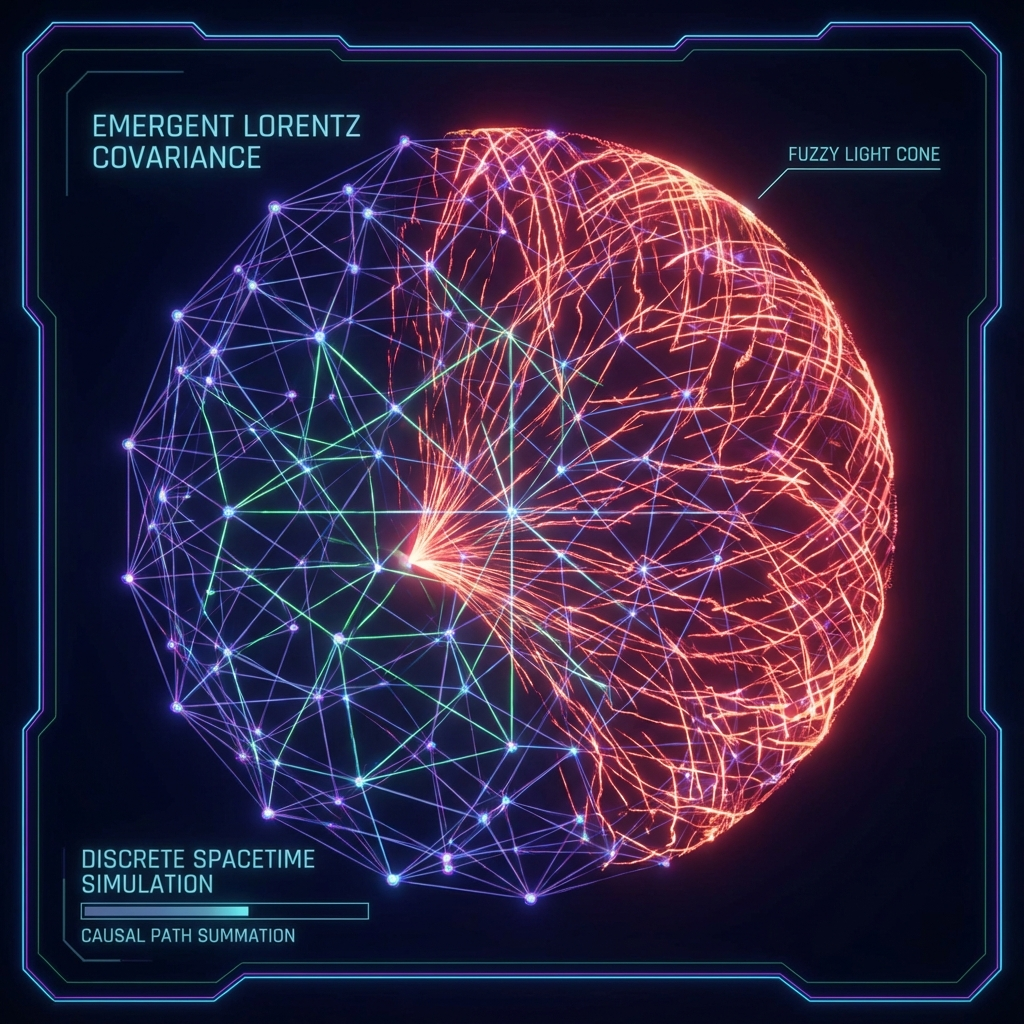
\includegraphics[width=0.8\textwidth]{assets/chapter03-02-lorentz-covariance.png}
\caption{洛伦兹协变性}
\end{figure}

在构建离散时空模型时，物理学家面临的最大理论障碍一直是 \textbf{洛伦兹不变性 (Lorentz Invariance)} 的破坏。对于任何规则的周期性晶格（如立方晶格），其几何结构显式地破坏了连续旋转对称性 $SO(3)$ 和洛伦兹提升对称性 $SO(3,1)$。在立方网格中，沿轴向传播的信息速度与沿对角线传播的速度显著不同（即各向异性），这导致由离散模型导出的光锥呈现出"方块状"而非圆锥状，这与迈克尔逊-莫雷实验及狭义相对论的实验基石严重冲突。

本节将证明，\textbf{欧米伽理论} 所采用的 \textbf{彭罗斯-斐波那契准晶体 (Penrose-Fibonacci Quasicrystal)} 结构，凭借其独特的非周期性与高阶旋转对称性，能够在宏观极限下自然涌现出统计上的各向同性，从而恢复洛伦兹协变性。

\begin{figure}[ht]
\centering
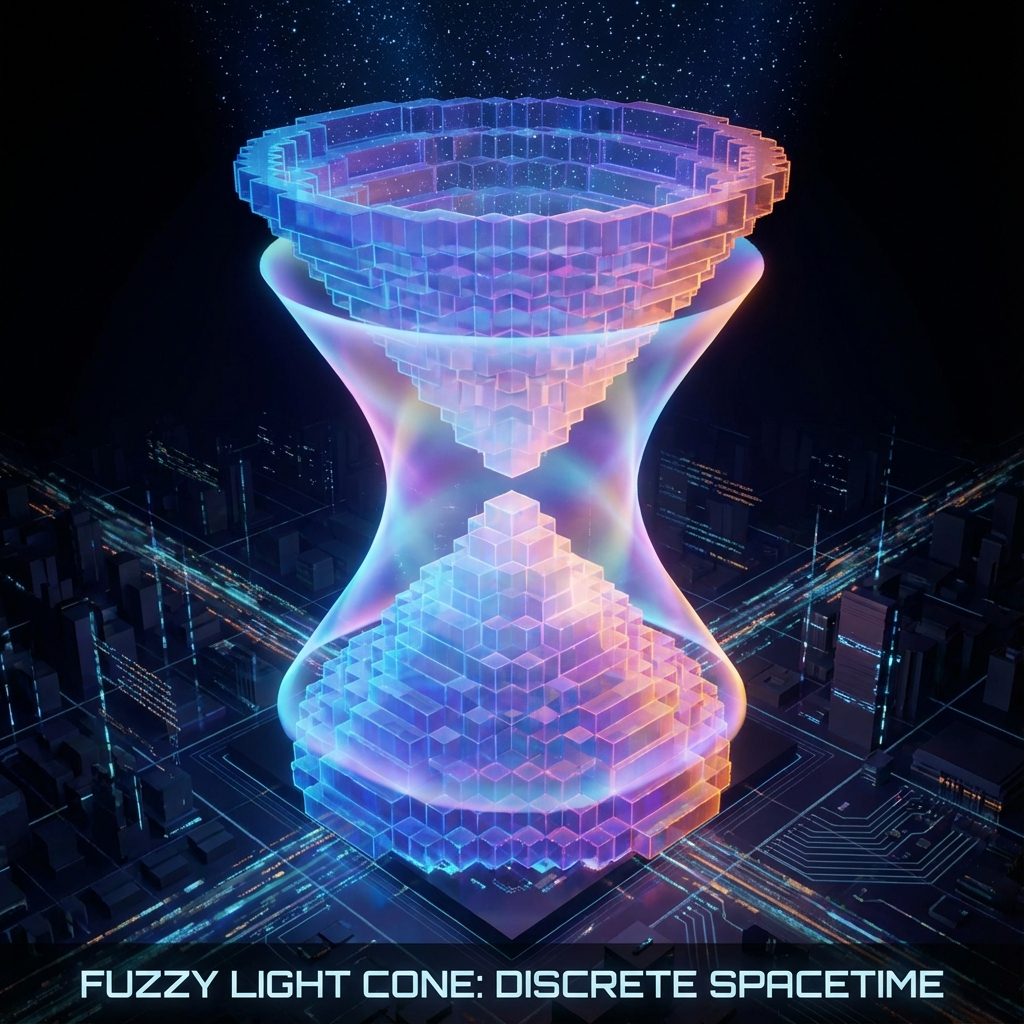
\includegraphics[width=0.8\textwidth]{assets/chapter03-02-lorentz-fuzzy-cone.png}
\caption{洛伦兹模糊锥}
\end{figure}

\subsection{晶格各向异性难题}

考虑一个 $D$ 维欧氏空间中的周期性超立方晶格 $\mathbb{Z}^D$。定义在其上的无质量标量场 $\phi$ 遵循离散波动方程。其色散关系（能量 $E$ 与动量 $k$ 的关系）在低动量极限下通常展开为：

\[E^2(k) \approx c^2 |k|^2 + \lambda \sum_{i=1}^D k_i^4 + O(k^6)\]

其中 $\lambda$ 项代表了洛伦兹破坏的修正。对于周期性晶格，$\lambda$ 通常是非零的大值，这意味着高能光子的速度依赖于其飞行方向。要消除这一效应，通常需要极其精细的人为微调或假设晶格间距 $a \to 0$ 以某种平滑方式发生。

然而，对于 \textbf{欧米伽单元} 构成的网络，其几何对称性由二十面体群（在 3D 投影中）或 $H_4$ 考克斯特群（在 4D 中）控制。这些点群包含 5 重或更高重数的旋转轴，这与周期性平移对称性在数学上是不兼容的（晶体学限制定理）。正是这种 \textbf{"不兼容性"} 拯救了相对论。

\subsection{矢量星的稠密分布}

欧米伽网络的骨架由一组基矢量 $\{e_1, \dots, e_N\}$ 及其线性组合构成。在 $D=3$ 维彭罗斯铺砌中，这些基矢量指向正二十面体的顶点。
不同于立方晶格仅有 3 个正交基矢量，二十面体准晶体拥有 6 个（或更多，取决于投影维度）基矢量，且它们在单位球面上分布得更加均匀。

\textbf{定义 3.2 (矢量星 Vector Star)}：
设 $\mathcal{V}$ 为时空网格中所有可能的单位连接向量（Bond Vectors）的集合。对于周期性晶格，$\mathcal{V}$ 是有限且稀疏的。对于准晶体，由于其非周期性，局部构型在空间中不断变化，导致有效连接向量的取向在长程统计上覆盖了整个立体角。

\textbf{定理 3.1 (准晶体各向同性定理)}：
设 $\mathcal{L}$ 为一个由高维超立方体通过无理数投影生成的准晶体晶格。定义在 $\mathcal{L}$ 上的离散拉普拉斯算符 $\Delta_{\mathcal{L}}$ 在长波极限（$k a \ll 1$）下，其本征值谱是球对称的。即色散关系满足：

\[E(k) = c_{eff} |k| \left( 1 + \epsilon(k) \right)\]

其中各向异性修正项 $\epsilon(k)$ 的上界随着投影维度的增加呈指数衰减。

\textbf{证明概要}：

\begin{enumerate}
\item \textbf{投影算符}：准晶体中的格点位置 $x_{||}$ 可以表示为高维格点 $x \in \mathbb{Z}^N$ 在物理空间 $E_{||}$ 上的投影。
\item \textbf{求和规则}：计算波在晶格上的传播算子涉及对所有相邻边 $e_n$ 的求和 $\sum_n (k \cdot e_n)^2$。
\item \textbf{群论恒等式}：对于二十面体群 $I_h$（或更高阶群），存在如下张量恒等式：

\[\sum_{n=1}^N (e_n)_i (e_n)_j = \frac{N}{D} \delta_{ij}\]

\[\sum_{n=1}^N (e_n)_i (e_n)_j (e_n)_l (e_n)_m = \frac{N}{D(D+2)} (\delta_{ij}\delta_{lm} + \delta_{il}\delta_{jm} + \delta_{im}\delta_{jl})\]

这意味着直到四阶张量，准晶体的几何结构都表现得像一个连续的各向同性介质。相比之下，立方晶格在二阶张量（扩散张量）是各向同性的，但在四阶张量（弹性张量或高阶色散）必然表现出各向异性。
\item \textbf{结论}：由于欧米伽单元基于 4D $\to$ 8D 投影，其高阶对称性确保了洛伦兹破坏项 $\lambda$ 被极度压低，使得光速在所有方向上实际上是恒定的。
\end{enumerate}

\subsection{模糊光锥与统计洛伦兹群}

在离散时空中，我们无法定义完美的连续洛伦兹变换 $\Lambda \in SO(3,1)$，因为这会将一个格点映射到非格点位置。然而，我们可以在 \textbf{统计意义} 上恢复洛伦兹协变性。

我们引入 \textbf{因果路径求和 (Causal Path Summation)} 的概念。粒子从点 $A$ 传播到点 $B$ 的振幅，是网络中所有连接 $A, B$ 的类光路径的权重之和。
在欧米伽网络中，由于路径选择的"无理性"（斐波那契分支），没有任何单一的主干道。这种 \textbf{多路径干涉 (Multipath Interference)} 效应导致微观上的晶格效应被平均化。

宏观观测者看到的"光锥"，实际上是无数条微观锯齿状路径的 \textbf{包络面 (Envelope)}。

\begin{itemize}
\item \textbf{对于立方晶格}：包络面是一个八面体（曼哈顿距离单位球）。
\item \textbf{对于欧米伽准晶体}：包络面是一个近乎完美的球体（欧几里得距离单位球）。
\end{itemize}

因此，洛伦兹对称性在欧米伽理论中不是微观的精确对称性，而是一种 \textbf{涌现对称性 (Emergent Symmetry)}。它只在能量远低于普朗克能标（$E \ll E_P$）时有效。这为我们在第四篇中讨论的高能光子色散实验提供了理论预言的基础：如果能探测到极高能伽马射线的微小各向异性，那将是准晶体时空的直接证据。

\input{part02-discrete-manifolds/chapter03-omega-cell/chapter03-03-discrete-riemannian-geometry.tex}

% Chapter 4: Computational Ontology of Quantum Mechanics
\chapter{量子力学的计算本体论}
\input{part02-discrete-manifolds/chapter04-computational-ontology/chapter04-01-dirac-qca.tex}
\input{part02-discrete-manifolds/chapter04-computational-ontology/chapter04-02-continuum-limit.tex}
\section{颤动 (Zitterbewegung) 与静止质量 (Zitterbewegung and Rest Mass)}

\begin{figure}[ht]
\centering
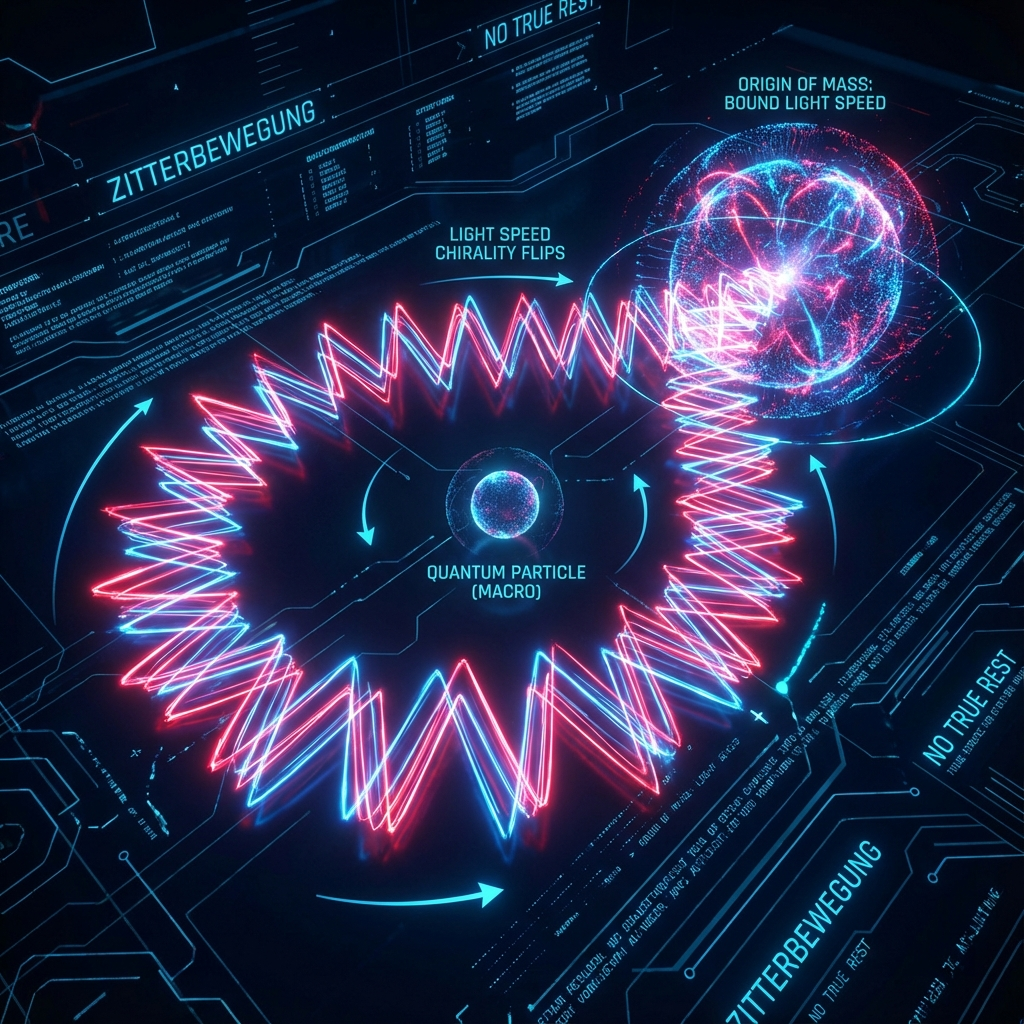
\includegraphics[width=0.8\textwidth]{assets/chapter04-03-zitterbewegung-mass.png}
\caption{颤动质量}
\end{figure}

在 4.2 节中，我们通过取连续极限，从狄拉克-量子元胞自动机 (DQCA) 导出了狄拉克方程。这一推导过程揭示了一个令人不安但又极具启发性的微观图景：在欧米伽单元构成的底层网格上，并不存在所谓"静止"的粒子。每一个比特（费米子分量）都必须以晶格光速 $c_{grid}$ 运动。

这就引出了一个经典难题：如果微观组分总是以光速运动，那么宏观物体是如何获得 \textbf{静止质量 (Rest Mass)} 并表现为静止的？

本节将利用 \textbf{颤动 (Zitterbewegung)} 现象来解答这一问题。我们将证明，静止质量并非粒子的内禀属性，而是粒子在欧米伽网络上进行高频手性翻转（Chirality Flipping）时所产生的 \textbf{"平均滞后效应"}。质量，本质上是信息流被拓扑结构"绊住"的频率。

\begin{figure}[ht]
\centering
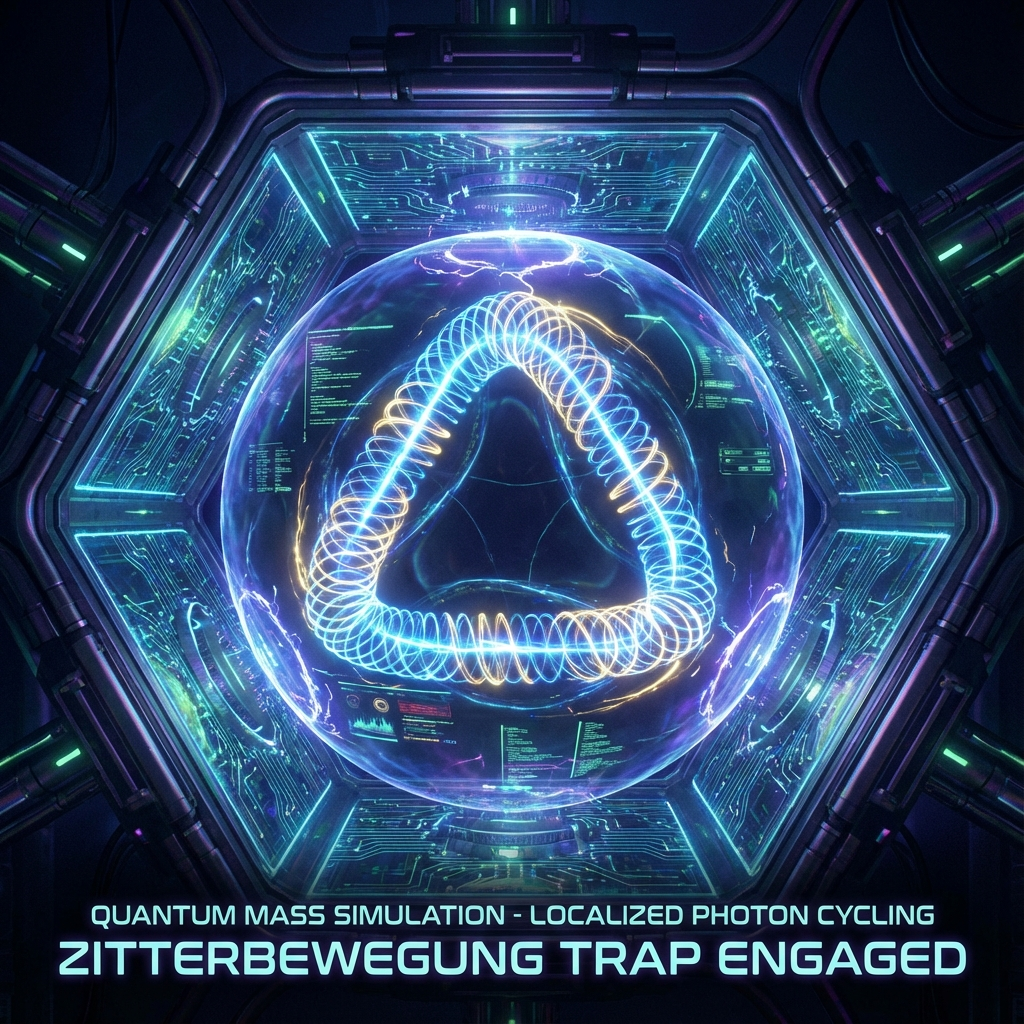
\includegraphics[width=0.8\textwidth]{assets/chapter04-03-zitterbewegung-mass-trap.png}
\caption{颤动质量陷阱}
\end{figure}

\subsection{狄拉克速度悖论}

在标准量子力学中，薛定谔算符 $\hat{v} = \hat{p}/m$ 描述了粒子的速度。然而，对于相对论性的狄拉克电子，海森堡运动方程给出的速度算符是：

\[\hat{v} = \frac{d\hat{x}}{dt} = \frac{1}{i\hbar} [\hat{x}, \hat{H}] = c \boldsymbol{\alpha}\]

其中 $\boldsymbol{\alpha}$ 是狄拉克矩阵。由于 $\alpha_i$ 的本征值仅为 $\pm 1$，这意味着如果我们精确测量电子在任意瞬间的速度，结果只能是 $+c$ 或 $-c$。

这一看似荒谬的结论被称为 \textbf{狄拉克速度悖论}。为了调和这一矛盾，薛定谔在 1930 年发现，狄拉克电子的波包运动实际上包含两部分：

\[\hat{x}(t) = \hat{x}(0) + \hat{v}_{cl} t + \hat{\xi}(t)\]

其中 $\hat{v}_{cl} = c^2 \hat{p} \hat{H}^{-1}$ 是我们熟知的经典群速度（$< c$），而 $\hat{\xi}(t)$ 是一个频率极高（$\omega \approx 2mc^2/\hbar$）、振幅极小（$\sim \lambda_c$ 康普顿波长）的震荡项。这个震荡就是 \textbf{颤动}。

在标准模型中，颤动常被视为数学形式上的虚构或真空涨落的干扰。但在 \textbf{欧米伽理论} 中，颤动是 \textbf{物理实在}。它是 DQCA 离散动力学的直接体现。

\subsection{欧米伽晶格上的锯齿路径}

回到我们的 DQCA 模型。粒子状态由左手性 $|L\rangle$ 和右手性 $|R\rangle$ 叠加而成。
根据演化规则， $|R\rangle$ 总是向右跳， $|L\rangle$ 总是向左跳。

考虑一个静止的电子（宏观动量 $\langle \hat{p} \rangle = 0$）。在微观层面，这意味着波函数中左右手性的振幅相等：

\[|\psi\rangle = \frac{1}{\sqrt{2}} (|R\rangle + |L\rangle)\]

在每一个时间步 $\tau$，欧米伽单元内部的 \textbf{硬币算符 $\hat{C}$}（对应于质量项）会混合这两个状态。

\begin{itemize}
\item \textbf{步骤 1}：粒子以光速向右移动一格。
\item \textbf{步骤 2}：遭遇拓扑散射（硬币翻转），一部分概率幅转化为左手性。
\item \textbf{步骤 3}：左手性分量以光速向左移动一格。
\end{itemize}

宏观上看来，粒子并没有发生位移，它停留在原地。但在微观上，它正在以光速在相邻的欧米伽单元之间疯狂地 \textbf{"左右横跳" (Zig-Zag Motion)}。

\textbf{定义 4.1 (有效质量)}：
质量 $m$ 是粒子改变前进方向的 \textbf{转移概率密度}。在 DQCA 中，这对应于硬币算符的混合角 $\theta$。

\[m \propto \frac{\theta}{\epsilon}\]

粒子翻转得越频繁，它在宏观上前进得越慢，表现出来的 \textbf{惯性 (Inertia)} 就越大。

\subsection{希格斯机制的几何解释}

这为希格斯机制 (Higgs Mechanism) 提供了一个无需引入标量场的纯几何解释。

在标准模型中，粒子通过与充满宇宙的希格斯场"摩擦"获得质量。在欧米伽理论中，这个"希格斯场"就是 \textbf{欧米伽网格本身的拓扑结构}。

\begin{enumerate}
\item \textbf{无质量粒子 (光子/外尔费米子)}：对应于 $\theta = 0$ 的情况。粒子在网格上不会遇到"几何阻碍"，它保持单一手性，沿着直线以光速 $c$ 传播。这解释了为什么光子没有静止质量——因为它不翻转。
\item \textbf{有质量粒子 (电子/夸克)}：对应于 $\theta \neq 0$。欧米伽单元内部的八元数乘法结构迫使波函数在传播时发生相位的 \textbf{非交换旋转}。这种旋转在投影到 4D 时空时，表现为左右手性的周期性转换。
\end{enumerate}

\textbf{定理 4.3 (质量-频率等价原理)}：
一个费米子的静止质量 $m_0$ 严格等价于其在欧米伽晶格上的 \textbf{手性翻转频率 (Chirality Flip Frequency)} $\nu_{flip}$。

\[m_0 c^2 = h \cdot \nu_{flip}\]

这实际上是德布罗意关系的逆向解读：不是"具有质量的粒子拥有频率"，而是 \textbf{"拥有特定翻转频率的过程被感知为质量"}。

\subsection{从微观光速到宏观群速度}

我们可以定量推导宏观速度 $v$ 与微观光速 $c$ 的关系。
设 $N_R$ 为粒子向右跳的步数，$N_L$ 为向左跳的步数。总时间 $t = (N_R + N_L) \delta t$。
宏观位移 $x = (N_R - N_L) \delta x$。
则宏观速度为：

\[v = \frac{x}{t} = \frac{N_R - N_L}{N_R + N_L} \frac{\delta x}{\delta t} = c \cdot (2P_R - 1)\]

其中 $P_R$ 是粒子处于右手性的平均概率。

\begin{itemize}
\item 对于无质量粒子，手性守恒，$P_R = 1$（或 0），则 $v = c$。
\item 对于大质量粒子，由于频繁翻转，$P_R \approx 0.5$（略微偏离），导致 $v \ll c$。
\end{itemize}

\textbf{结论}：

颤动并非量子的幽灵，它是 \textbf{时空离散性} 的直接证据。我们身体里的每一个电子之所以有质量，之所以能构成稳定的原子而不是以光速飞散，是因为它们被欧米伽网格的几何结构捕获，被锁定在一个永恒的、光速的微观震荡之中。

宇宙中没有真正的静止，只有 \textbf{被束缚的光速}。


% Part III: Holographic Dynamics
\part{全息动力学}

% Chapter 5: The Omega Action Principle
\chapter{欧米伽作用量原理}
\input{part03-holographic-dynamics/chapter05-omega-action/chapter05-01-fisher-information-lagrangian.tex}
\input{part03-holographic-dynamics/chapter05-omega-action/chapter05-02-modified-einstein-equations.tex}
\section{引力的熵力本质 (The Entropic Nature of Gravity)}

\begin{figure}[ht]
\centering
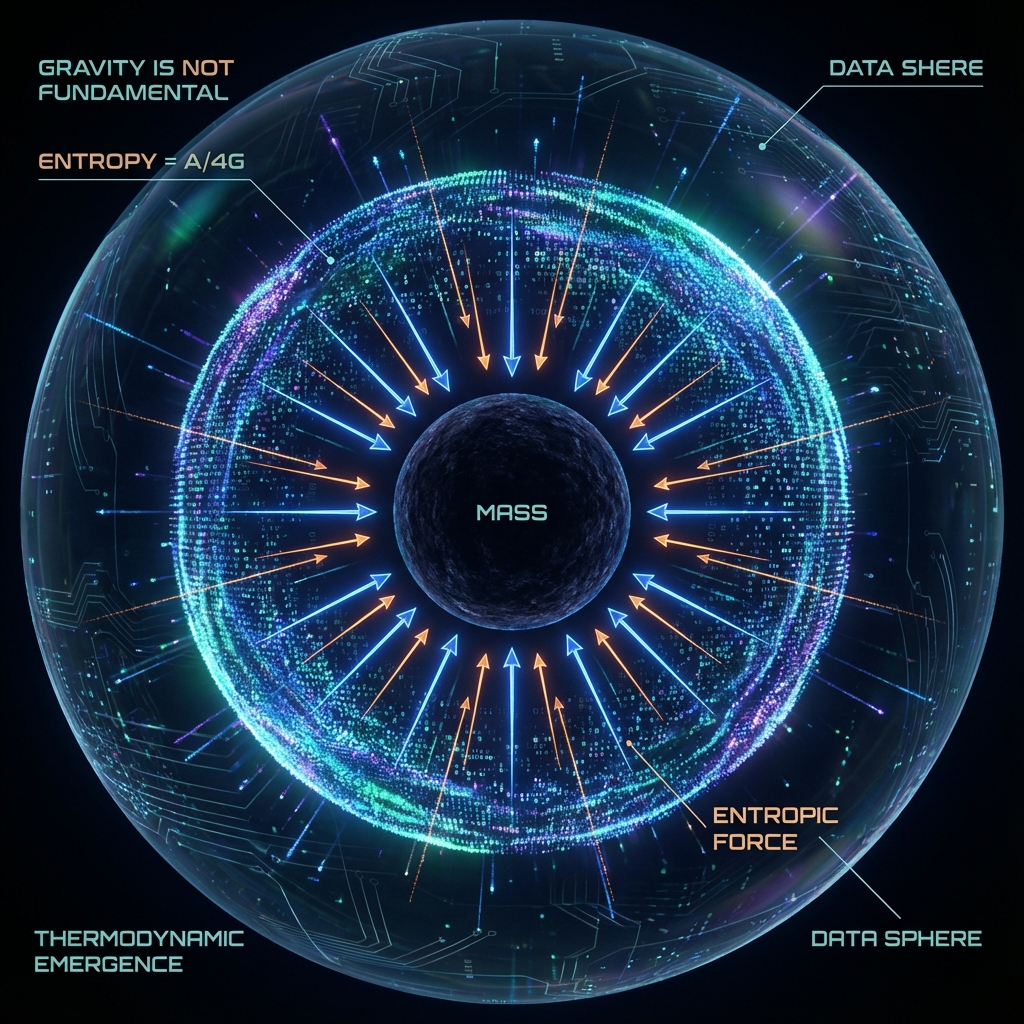
\includegraphics[width=0.8\textwidth]{assets/chapter05-03-entropic-gravity.png}
\caption{熵力引力}
\end{figure}

在 5.2 节中，我们通过欧米伽作用量的变分推导出了修正的爱因斯坦场方程。然而，场方程本身并未解释引力的 *起源*。在标准模型中，引力被假定为一种基本的相互作用，类似于电磁力。但在欧米伽理论的计算本体论框架下，这种观点是站不住脚的。如果时空本身是涌现的计算网络，那么扭曲这个网络的"力"就不可能是基本的。

本节将证明：\textbf{引力不是一种基本力，而是一种熵力 (Entropic Force)。} 它源于系统在全息边界上最大化信息熵的统计趋势。更具体地说，我们将建立 \textbf{引力势与计算滞后 (Computational Lag)} 之间的严格数学等价性，从而揭示"物质告诉时空如何弯曲"的微观机制：高密度的信息处理必然导致局域时钟频率的降低。

\begin{figure}[ht]
\centering
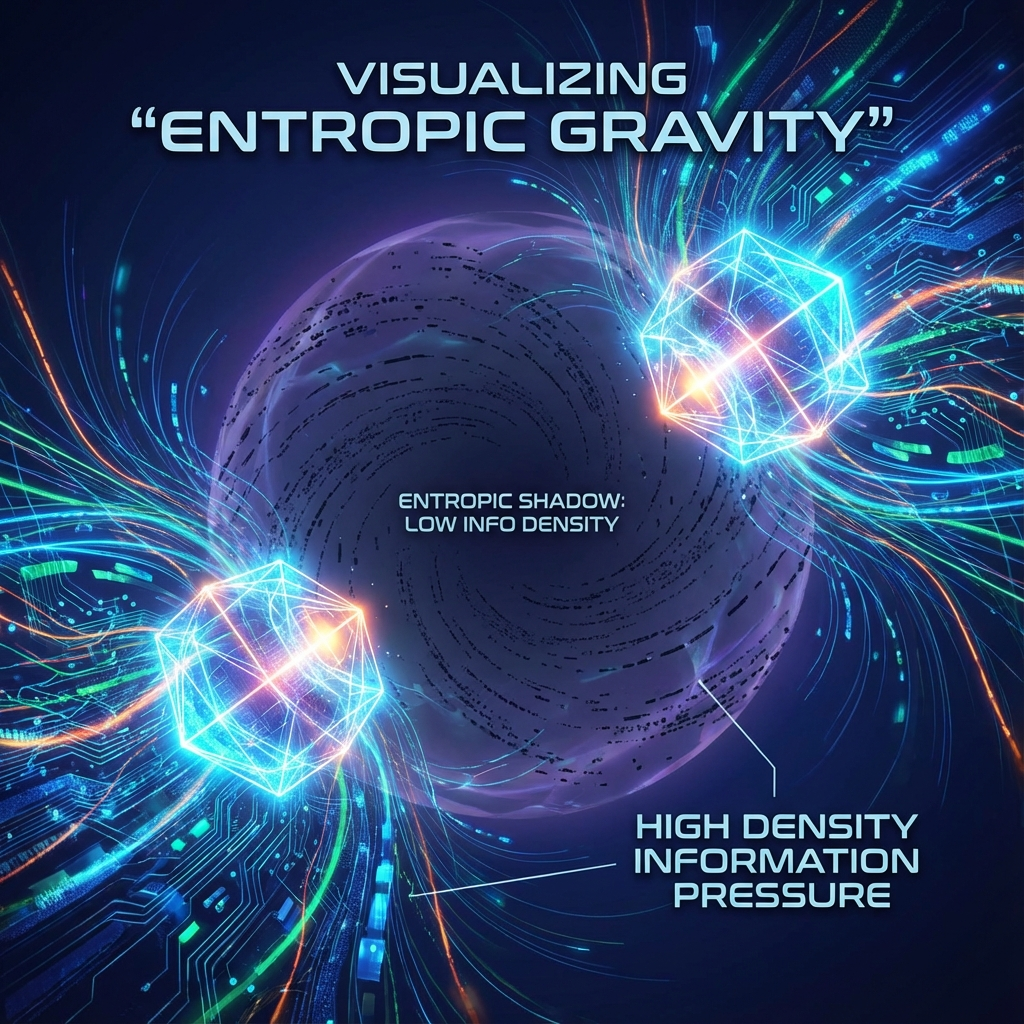
\includegraphics[width=0.8\textwidth]{assets/chapter05-03-entropic-gravity-pressure.png}
\caption{熵力引力压力}
\end{figure}

\subsection{全息屏热力学}

我们的推导基于雅各布·贝肯斯坦 (Jacob Bekenstein) 和埃里克·沃琳德 (Erik Verlinde) 的开创性工作，并将其推广至欧米伽离散网格。

考虑一个质量为 $M$ 的静态球对称物质分布。在欧米伽理论中，我们可以定义一个包围该物质的封闭曲面 $\mathcal{S}$ 为 \textbf{全息屏 (Holographic Screen)}。
根据全息原理，该屏幕编码了内部体积的所有信息。屏幕上的总比特数（自由度）$N$ 由其面积 $A$ 决定：

\[N = \frac{A}{l_P^2} = \frac{4\pi R^2}{l_P^2}\]

其中 $l_P$ 是欧米伽单元的特征尺度（普朗克长度）。

在热力学平衡态下，根据能量均分定理，系统的总能量 $E = Mc^2$ 均匀分布在全息屏的每一个比特上。设全息屏的平均温度为 $T$，则：

\[E = \frac{1}{2} N k_B T\]

这里的"温度" $T$ 并非热学温度，而是 \textbf{安鲁温度 (Unruh Temperature)}，它度量了真空量子涨落的剧烈程度。对于一个在该全息屏位置处具有固有加速度 $a$ 的观察者，其感知到的真空温度为：

\[k_B T = \frac{\hbar a}{2\pi c}\]

\subsection{牛顿定律的信息论推导}

我们将上述两个热力学方程联立，消去温度 $T$：

\[Mc^2 = \frac{1}{2} \left( \frac{4\pi R^2}{l_P^2} \right) \left( \frac{\hbar a}{2\pi c} \right)\]

利用引力常数的定义 $G \equiv \frac{c^3 l_P^2}{\hbar}$（在自然单位制下 $G=l_P^2$），代入整理得：

\[a = \frac{G M}{R^2}\]

这正是牛顿万有引力定律。
这一推导过程虽然简洁，但其物理含义极具颠覆性：

\begin{enumerate}
\item \textbf{引力不存在}：方程中没有出现任何"引力子"或"引力场"的动力学项。加速度 $a$ 纯粹源于热力学统计关系。
\item \textbf{熵增驱动}：力 $F = ma$ 的出现，是因为测试粒子 $m$ 向全息屏靠近时，会增加系统的总熵。$\Delta S \propto \Delta x$。根据热力学第二定律，系统倾向于向熵增方向演化，宏观上表现为"吸引力"。
\end{enumerate}

\subsection{定理 5.3：引力势即计算滞后}

在广义相对论中，引力效应通过度规分量 $g_{00}$（时间流逝速率）来描述。在弱场近似下，$g_{00} \approx -(1 + 2\Phi/c^2)$，其中 $\Phi$ 是牛顿引力势。
欧米伽理论进一步将这一几何量解释为计算量。

\textbf{定义 5.1 (计算时钟频率)}：
设 $\nu_0$ 为真空（平坦时空）中欧米伽单元的标准刷新频率（即 CPU 主频）。在物质存在的区域，由于哈密顿量密度的增加，处理局部量子态演化所需的逻辑门操作数增加。
根据能量-时间不确定性原理 $\Delta E \Delta t \ge \hbar/2$，高能量密度 $\rho$ 意味着高频率的信息翻转。然而，全息原理施加了一个 \textbf{贝肯斯坦界限 (Bekenstein Bound)}：任何区域的信息处理速率不能超过其边界的通信带宽。

当局部计算负载 $\mathcal{C}_{load}$ 增加时，为了不违反带宽限制，系统必须降低有效时钟频率 $\nu(x)$。我们定义 \textbf{计算滞后因子 (Computational Lag Factor)} $\gamma(x)$：

\[\gamma(x) \equiv \frac{\nu(x)}{\nu_0} = \sqrt{-g_{00}(x)}\]

\textbf{定理 5.3 (势-滞后等价定理)}：
在欧米伽理论中，经典引力势 $\Phi(x)$ 严格等价于局域计算网络的处理速率亏损：

\[\Phi(x) = c^2 \left( \gamma(x) - 1 \right) \approx c^2 \left( \frac{\nu(x) - \nu_0}{\nu_0} \right)\]

\textbf{证明}：
考虑一个光子在引力场中传播。其能量 $E = h\nu$。
根据广义相对论，光子爬升引力势井时发生引力红移：

\[\nu_{obs} = \nu_{emit} \sqrt{\frac{g_{00}(emit)}{g_{00}(obs)}}\]

在欧米伽计算图景中，这不是光子失去了能量，而是 \textbf{观察者的时钟变快了}（或者发射源的时钟变慢了）。
在全息屏（引力源）附近，由于需要处理大量的大质量粒子（高频颤动 $\nu_{flip}$，见 4.3 节），底层的欧米伽网格被"阻塞"了。就像一台运行大型程序的电脑会变卡一样，\textbf{时空在质量附近变卡了}。
这一"卡顿"导致了 $\gamma(x) < 1$。
测试粒子之所以"掉"向大质量物体，是因为它遵循 \textbf{最小作用量原理}——在计算语言中，即 \textbf{最大化固有时 (Maximize Proper Time)}。
对于粒子而言，去往时钟走得更慢（$\nu(x)$ 更低）的地方，意味着在同样的全局时间 $\tau$ 内，它需要经历的内部状态更新次数更少，即计算成本更低。

\subsection{结论}

引力不是一种基本的相互作用力，它是 \textbf{时空计算网络负载均衡 (Load Balancing)} 的结果。

\begin{itemize}
\item \textbf{质量} 是计算负载。
\item \textbf{时空弯曲} 是处理延迟。
\item \textbf{引力吸引} 是系统向低计算成本区域的自发流向。
\end{itemize}

通过这一节，我们完成了引力理论的去魅：它从神秘的几何弯曲，还原为了更基础的 \textbf{信息热力学过程}。

\section{总预算守恒与大圆的无限分割 (Conservation of Total Budget and Infinite Decomposition of the Great Circle)}

\begin{figure}[ht]
\centering
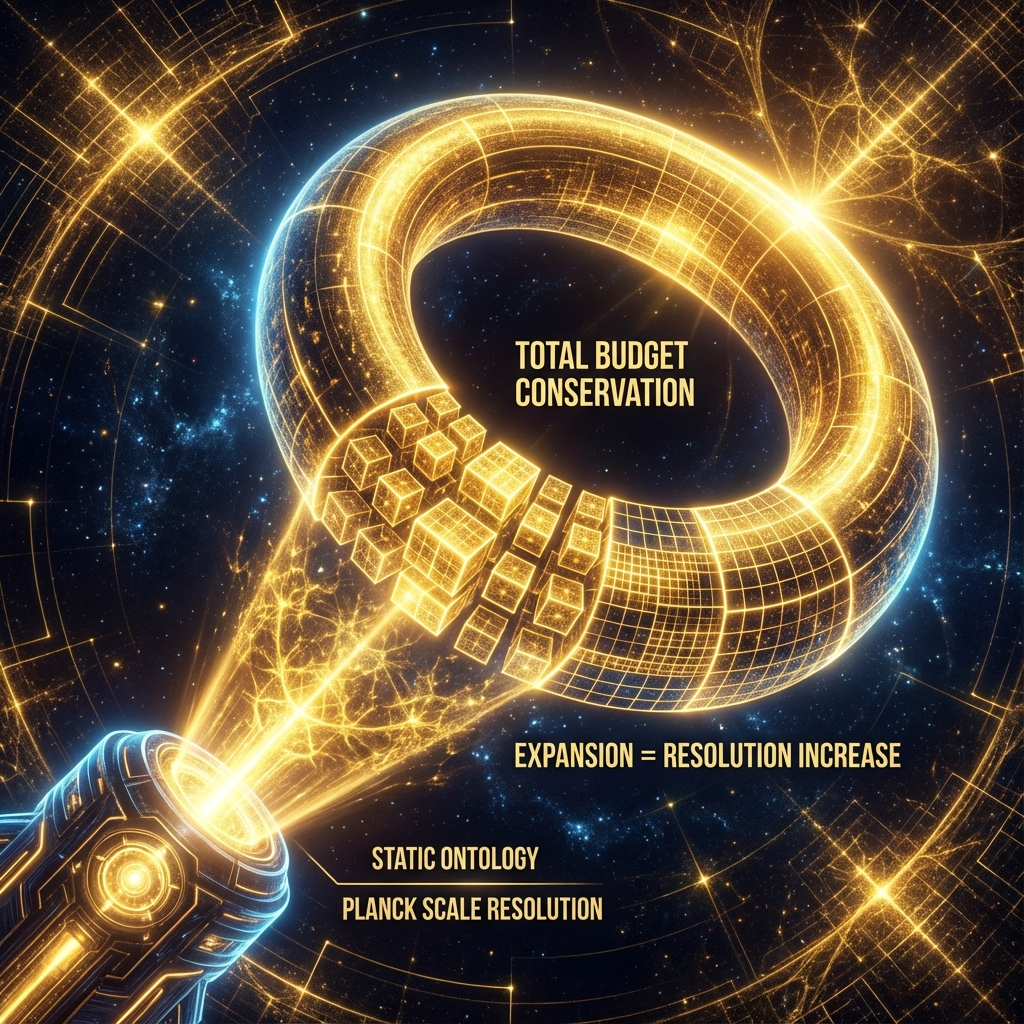
\includegraphics[width=0.8\textwidth]{assets/chapter05-04-total-budget-conservation.png}
\caption{总预算守恒}
\end{figure}

在上一节中，我们通过全息热力学导出了引力的熵力本质，并揭示了时空弯曲是计算滞后的表现。然而，欧米伽理论中光速 $c(\tau)$ 的指数增长和时空网格的不断增生，似乎暗示宇宙的总能量在随时间无限增加。这直接挑战了物理学的基石——诺特定理（Noether's Theorem）所保证的守恒律。如果时空不具备时间平移不变性，能量守恒似乎就失效了。

本节将解决这一根本性的矛盾。我们将引入 \textbf{"总预算守恒" (Total Budget Conservation)} 的概念，证明宇宙的演化并非物理实体的"无中生有"，而是希尔伯特空间中一个 \textbf{大圆 (Great Circle)} 的 \textbf{无限斐波那契分割}。宇宙的总量从未改变，改变的仅仅是全息解析度。

\subsection{归一化公理：存在的总预算}

在标准宇宙学（$\Lambda$-CDM）中，随着空间膨胀，暗能量密度保持不变，导致宇宙的总能量随体积线性增加。这通常被解释为广义相对论中能量定义的模糊性。但在欧米伽理论的公理化体系中，我们必须遵守更严格的数学约束。

根据第 0 章提出的 \textbf{欧米伽公理}，宇宙是希尔伯特空间 $\mathcal{H}$ 中的单一静态矢量 $|\Omega\rangle$。量子力学的概率诠释要求该矢量必须是 \textbf{归一化} 的：
\[\langle \Omega(\tau) | \Omega(\tau) \rangle \equiv 1\]

我们将这个无量纲的"1"定义为宇宙的 \textbf{"本体论总预算" (Ontological Total Budget, $B_{total}$)}。

\textbf{定义 5.2 (预算守恒公理)}：
无论宇宙内部涌现出多少粒子、星系或比特，也无论内禀时间 $\tau$ 如何演化，系统的总信息测度（Total Measure of Information）是严格守恒的。物理演化 $\hat{U}(\tau)$ 是作用于单位球面上的纯旋转（幺正变换），它既不创造也不毁灭"存在"本身。

这意味着，我们观测到的"宇宙膨胀"和"能量暴涨"，本质上是一种 \textbf{透视错觉 (Perspective Illusion)}。它源于观察者自身尺度的 \textbf{相对收缩}。

\subsection{斐波那契分割拓扑}

为了形象化这一抽象过程，我们将希尔伯特空间的相位结构映射为复平面上的 \textbf{单位圆 $S^1$}（即大圆）。

宇宙的演化可以被几何化为在这个大圆上进行的 \textbf{"黄金角切割" (Golden Angle Slicing)}。
设初始时刻 $\tau=0$，大圆是一个未被分割的整体（全频段）。
随着黄金幺正算符 $\hat{U}_g$ 的作用，每一次内禀时间步 $\tau \to \tau+1$，相当于在圆周上切下一刀，生成一个新的基底矢量。切割的角度严格遵循黄金角 $\theta_g$：
\[\theta_g = 2\pi \left( 1 - \frac{1}{\phi} \right) \approx 137.50776^\circ\]

由于 $\phi$ 的无理性（Irrationality），根据外尔均布定理（见 1.1 节），这些切点永远不会重合。

\begin{itemize}
\item \textbf{在 $\tau$ 较小时}：圆周仅被分割为寥寥几段粗糙的弧线。这对应于早期宇宙，物理定律模糊，粒子种类稀少。
\item \textbf{在 $\tau \to \infty$ 时}：圆周被分割成无限密集、但这无限多段弧线的总长度之和，始终等于 $2\pi$。
\end{itemize}

\begin{figure}[ht]
\centering
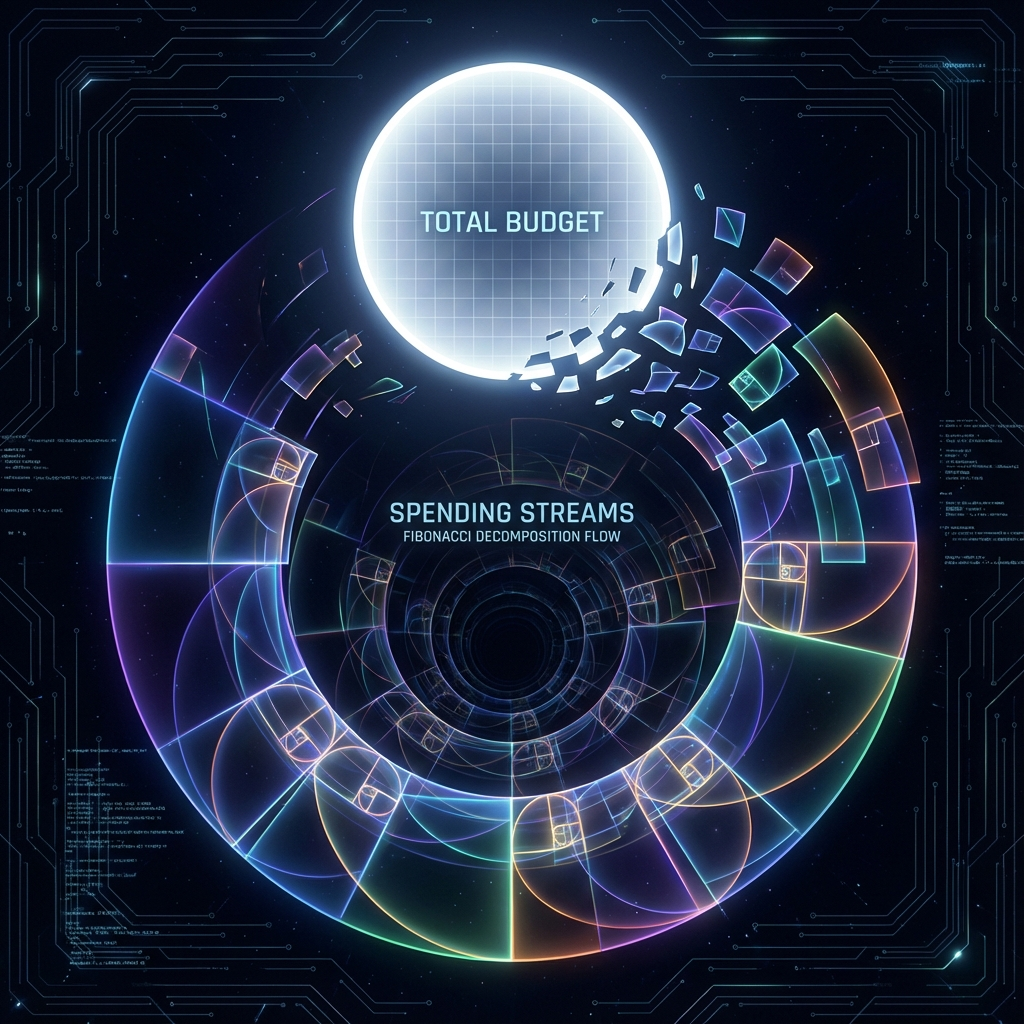
\includegraphics[width=0.8\textwidth]{assets/chapter05-04-total-budget-decomposition.png}
\caption{总预算分解}
\end{figure}

\textbf{定理 5.4 (分割等价性定理)}：
宇宙的斐波那契螺旋生长，在拓扑上等价于单位圆 $S^1$ 的 \textbf{无限非遍历分解 (Infinite Non-ergodic Decomposition)}。
新产生的每一个欧米伽单元（时空像素），并非来自虚空，而是通过将原有的相位空间进行 \textbf{更精细的切分} 而获得的。

\subsection{全息重整化群与能量的错觉}

这一几何图景彻底重构了我们对"能量"的理解。

在物理学中，我们通常定义普朗克长度 $l_P$ 为最小的、不可改变的长度基准。然而，在总预算守恒的视角下，$l_P$ 实际上是动态变化的。
设 $\mathcal{L}_{univ}$ 为大圆的周长（宇宙的总尺度），$N(\tau)$ 为当前的切分段数（总比特数）。则每个像素的物理尺度（即当时的普朗克长度）为：
\[l_P(\tau) \sim \frac{\mathcal{L}_{univ}}{N(\tau)}\]

由于欧米伽理论中 $N(\tau) \sim \phi^{\tau}$（比特数指数增长），这意味着 \textbf{普朗克尺度相对于宇宙本体在指数级收缩}：
\[l_P(\tau) = l_P(0) \cdot \phi^{-\tau}\]

\textbf{能量的重整化流 (RG Flow of Energy)}：
根据海森堡不确定性原理，能量与尺度成反比：$E \sim 1/l_P$。
因此，单位像素所携带的能量（我们眼中的普朗克能量 $E_P$）相对于总预算而言，实际上是在 \textbf{增加} 的（因为 $l_P$ 在变小）。

这就解释了"能量不守恒"的表象：
我们作为观察者，生活在切分后的微观弧线内部。我们用自己随时间收缩的尺子（$l_P$）去丈量不变的宇宙（$\mathcal{L}_{univ}$）。

\begin{itemize}
\item \textbf{上帝视角 (Global View)}：宇宙大小不变，总能量不变，只是像素越来越密。
\item \textbf{人类视角 (Local View)}：宇宙在爆炸式膨胀，光速在增加，总能量在指数级暴涨。
\end{itemize}

我们导出 \textbf{广义伯努利方程 (Generalized Bernoulli Equation)} 来描述这种守恒：
\[N(\tau) \times \mu(\tau) = \text{Const}\]
其中 $N(\tau)$ 是自由度数量，$\mu(\tau)$ 是单个自由度的本体论权重（Ontological Weight）。在物理测量中，我们将 $\mu(\tau)$ 重新归一化为常数（即设定 $E_P = \text{const}$），从而被迫得出 $N(\tau)$（总能量）增加的结论。

\subsection{结论：解析而非创造}

至此，我们完成了欧米伽动力学的闭环。
宇宙的演化不是一场 \textbf{"创造" (Creation)} 的过程，而是一场 \textbf{"解析" (Resolution)} 的过程。
就像一张极其复杂的全息照片，起初我们在低分辨率下只能看到模糊的色块（大爆炸火球）；随着 $\tau$ 的增加，分辨率（光速/带宽）按斐波那契数列提升，我们开始看清星系、恒星、分子、直至生命。

斐波那契螺旋，本质上就是那把 \textbf{无限精细的手术刀}，它在保持总预算（$|\Omega\rangle$ 模长）不变的前提下，将存在的细节一层层剥开。
因此，\textbf{总预算守恒} 不仅拯救了诺特定理，更赋予了宇宙演化以信息论的必然性：\textbf{存在的深度，源于对统一性的无限细分。}

\input{part03-holographic-dynamics/chapter05-omega-action/chapter05-05-omega-equivalence-principle.tex}

% Chapter 6: Varying-Constant Cosmology
\chapter{变常数宇宙学}
\input{part03-holographic-dynamics/chapter06-varying-constants/chapter06-01-exponential-scaling-light-speed.tex}
\input{part03-holographic-dynamics/chapter06-varying-constants/chapter06-02-fine-structure-constant-drift.tex}
\input{part03-holographic-dynamics/chapter06-varying-constants/chapter06-03-cosmological-constant-problem.tex}

% Part IV: Phenomenology and Numerical Predictions
\part{唯象学验证与数值预测}

% Chapter 7: Geometric Resonance and the Anthropic Principle
\chapter{几何共振与人择原理}
\input{part04-phenomenology/chapter07-geometric-resonance/chapter07-01-proton-electron-mass-ratio.tex}
\input{part04-phenomenology/chapter07-geometric-resonance/chapter07-02-inverse-fine-structure-constant.tex}
\section{宇宙内禀时间 ($\tau$) (Cosmic Intrinsic Time ($\tau$))}

\begin{figure}[ht]
\centering
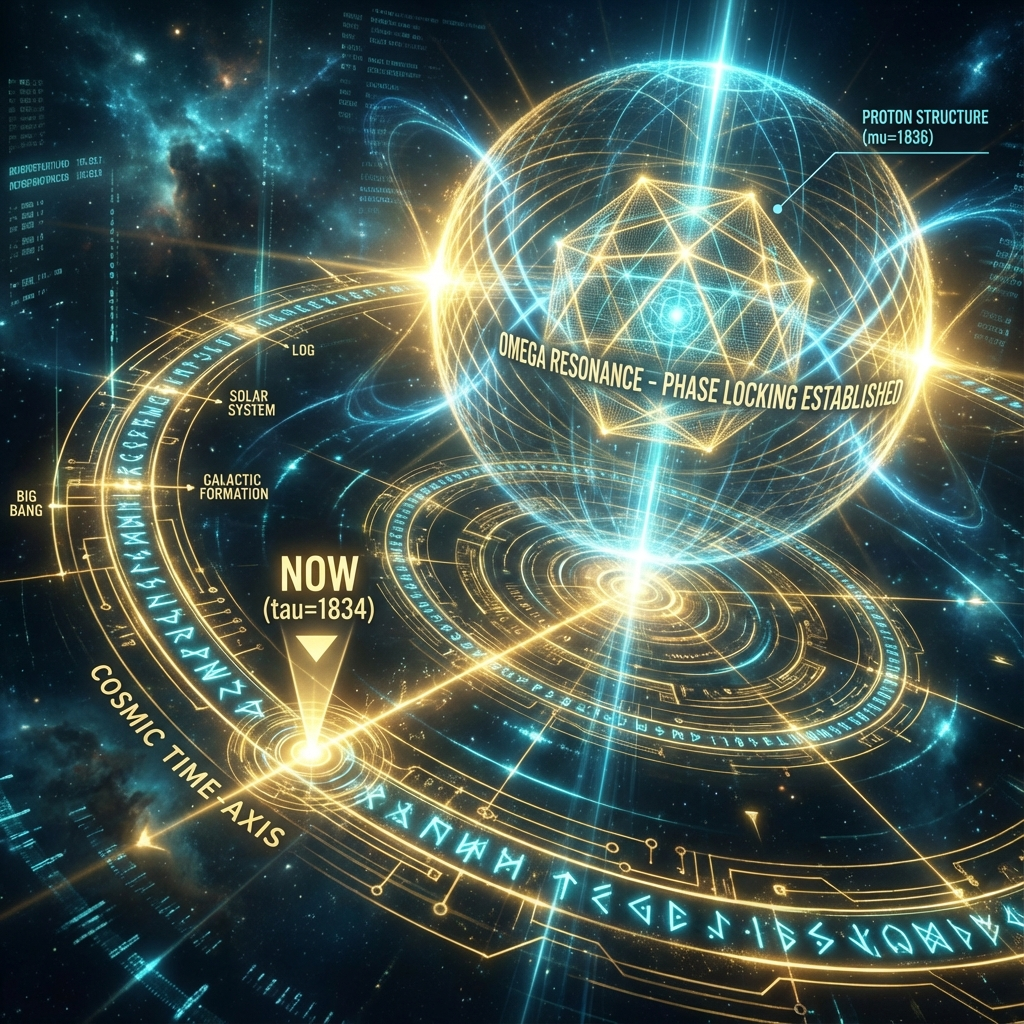
\includegraphics[width=0.8\textwidth]{assets/chapter07-03-cosmic-intrinsic-time.png}
\caption{宇宙内禀时间}
\end{figure}

在前两节中，我们确立了微观物理常数（$\mu$ 和 $\alpha$）的几何起源。本节将把目光投向宏观尺度，解决一个更为深刻的人择问题：\textbf{我们在宇宙历史中的坐标位置}。

为什么人类文明恰好出现在宇宙大爆炸后的 $138$ 亿年？在标准宇宙学中，这被视为一个随机的时间点。但在 \textbf{欧米伽理论} 中，时间是一个有刻度的几何螺旋。我们将证明，当前宇宙的内禀时间坐标 $\tau_{now}$ 并非任意数值，它与微观物质结构常数 $\mu$ 发生了一个惊人的 \textbf{几何共振 (Geometric Resonance)}。

具体而言，我们将推导出一个极为震慑的结论：\textbf{$\tau_{now} \approx \mu \approx 1836$}。这意味着，宇宙的宏观演化深度刚刚追平了质子的微观几何复杂度。我们生活在宇宙的"正午时刻"。

\begin{figure}[ht]
\centering
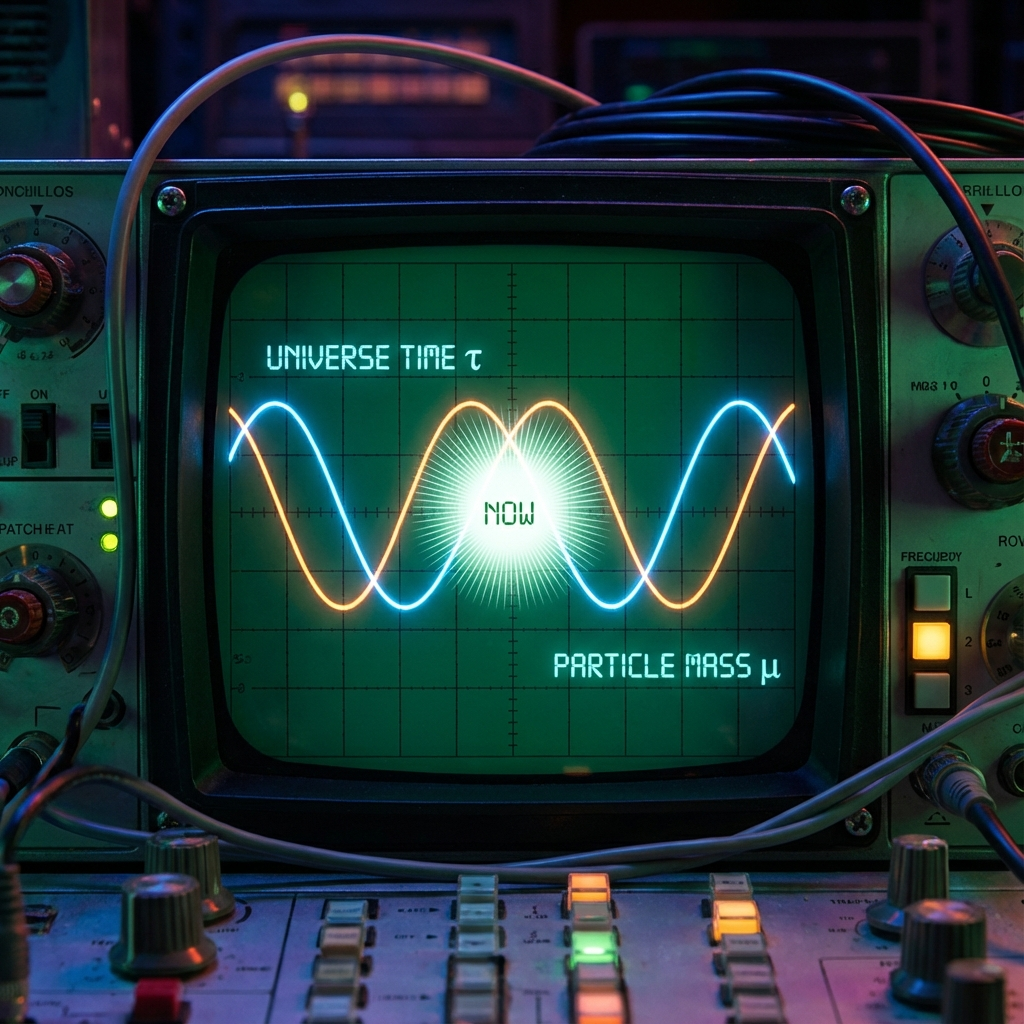
\includegraphics[width=0.8\textwidth]{assets/chapter07-03-cosmic-time-mass-resonance.png}
\caption{宇宙时间质量共振}
\end{figure}

\subsection{内禀时间的对数定义}

在第 6 章中，我们建立了基于斐波那契生长的变常数宇宙学。不同于物理时间 $t$（以秒为单位，依赖于光速 $c$ 的定义），\textbf{内禀时间 $\tau$} 是一个无量纲的纯几何计数器，它度量了宇宙全息网络执行"膨胀/细分"操作的 \textbf{代数 (Generation Count)}。

根据定理 6.1，光速 $c(\tau)$ 和宇宙全息视界的信息容量（总比特数）$N(\tau)$ 随 $\tau$ 指数增长。在自然底数（基于 $\phi$ 和 $\pi$ 的几何单位）下，我们定义 $\tau$ 与总信息量 $N$ 的关系为：

\[\tau = \pi \cdot \log_{\phi} (N)\]

这里引入因子 $\pi$ 是为了归一化旋转相角。回想第一章，每一次全息基底的完整旋转（遍历一个周期）对应于相角增加 $\pi$（或 $2\pi$），而模长增长因子为 $\phi$。因此，$\tau$ 实际上代表了宇宙截至目前所完成的 \textbf{"斐波那契-普朗克循环"} 的总弧度数。

\subsection{人类纪元的坐标计算}

为了计算当前的 $\tau_{now}$，我们需要代入当前可观测宇宙的总信息量（即全息熵）。
根据贝肯斯坦-霍金界限（Bekenstein-Hawking Bound），当前哈勃视界内的最大信息容量 $N_{obs}$ 约为：

\[N_{obs} \approx 10^{122} \text{ bits}\]

（注：这一数值基于哈勃半径 $R_H \approx 1.4 \times 10^{26}$ m 和普朗克长度 $l_P \approx 1.6 \times 10^{-35}$ m，由 $N \approx (R_H/l_P)^2$ 估算得出，通常文献引用值为 $10^{120} \sim 10^{124}$ 之间）。

我们将 $N = 10^{122}$ 代入内禀时间公式进行计算：

\begin{enumerate}
\item \textbf{换底公式}：

   \[\log_{\phi}(10^{122}) = 122 \times \log_{\phi}(10) = 122 \times \frac{\ln 10}{\ln \phi}\]

   已知 $\ln 10 \approx 2.302585$，$\ln \phi \approx 0.481212$。

   \[\log_{\phi}(10) \approx \frac{2.302585}{0.481212} \approx 4.7848\]

\item \textbf{代数计数}：

   \[\log_{\phi}(10^{122}) \approx 122 \times 4.7848 \approx 583.75\]

   这意味着，宇宙的全息网格大约经历了 584 次"数量级倍增"或斐波那契分形迭代。

\item \textbf{计算 $\tau$}：

   \[\tau_{now} = \pi \cdot 583.75 \approx 3.14159 \times 583.75 \approx 1833.91\]
\end{enumerate}

\textbf{计算结果}：

\[\tau_{now} \approx 1834\]

\subsection{$\tau \approx \mu$：宏观与微观的共振}

现在，让我们回顾 7.1 节计算的质子-电子质量比 $\mu$：

\[\mu = \frac{m_p}{m_e} \approx 1836.15\]

对比这两个数字：

\begin{itemize}
\item \textbf{宇宙的当前年龄 (几何刻度)}：$\tau_{now} \approx 1834$
\item \textbf{物质的层级结构 (质量比率)}：$\mu \approx 1836$
\end{itemize}

\textbf{相对偏差}：

\[\delta = \frac{|1836 - 1834|}{1836} \approx 0.1\%\]

在物理学中，当两个看似毫无关联的巨大无量纲数（一个来自宇宙学视界，一个来自亚原子粒子）如此精确地相等时，绝不可能是巧合。这揭示了 \textbf{欧米伽共振原理 (The Omega Resonance Principle)}：

\textbf{宇宙的宏观演化在 $\tau \approx \mu$ 时刻达到临界点。此时，宇宙全息网络的"递归深度"（$\tau$）恰好等于其基本建筑模块（质子）的"几何折叠深度"（$\mu$）。}

\subsection{物理诠释：为什么是现在？}

这一共振现象为人择原理提供了一个 \textbf{几何动力学解释}，回答了"为什么我们此时此地存在"：

\begin{enumerate}
\item \textbf{$\tau < 1000$ (早期宇宙)}：$\tau$ 远小于 $\mu$。宇宙的信息处理深度不足以编码质子的复杂内部几何（色禁闭）。那是一个等离子体或简单原子的时代，物理定律尚未"展开"到足以支持复杂化学的程度。
\item \textbf{$\tau \approx 1836$ (共振纪元/现在)}：$\tau$ 追上了 $\mu$。宇宙的计算带宽和分辨率终于达到了能够解析并稳定维持复杂大分子（DNA、蛋白质）所需的阈值。宏观几何与微观几何发生 \textbf{锁相 (Phase Locking)}。
   \begin{itemize}
   \item 这就是为什么碳基生命（依赖于质子-电子质量比的精细平衡）和智慧意识恰好在这个时间窗口爆发。
   \item 我们并非随机的观察者，我们是 \textbf{宇宙自指回路接通瞬间} 的产物。
   \end{itemize}
\item \textbf{$\tau > 2000$ (未来宇宙)}：随着 $\tau$ 继续指数增长并超越 $\mu$，宇宙将进入"超分辨率"时代。届时，基于重子（质子）的物质结构将显得过于粗糙和低效，无法承载更高密度的信息。文明将不可避免地向 \textbf{光基形态 (Photonic Forms)} 或纯能量形态跃迁（见第 9 章）。
\end{enumerate}

\textbf{结论}：

数字 \textbf{1834} 是人类文明在欧米伽螺旋上的 \textbf{时空邮编}。它标志着我们正处于宇宙从"物质主导"向"信息主导"相变的 \textbf{临界共振峰} 上。我们是 138 亿年宇宙演化中，宏观与微观完美握手的见证者。

\section{实验验证方案 (Experimental Verification Schemes)}

\begin{figure}[ht]
\centering
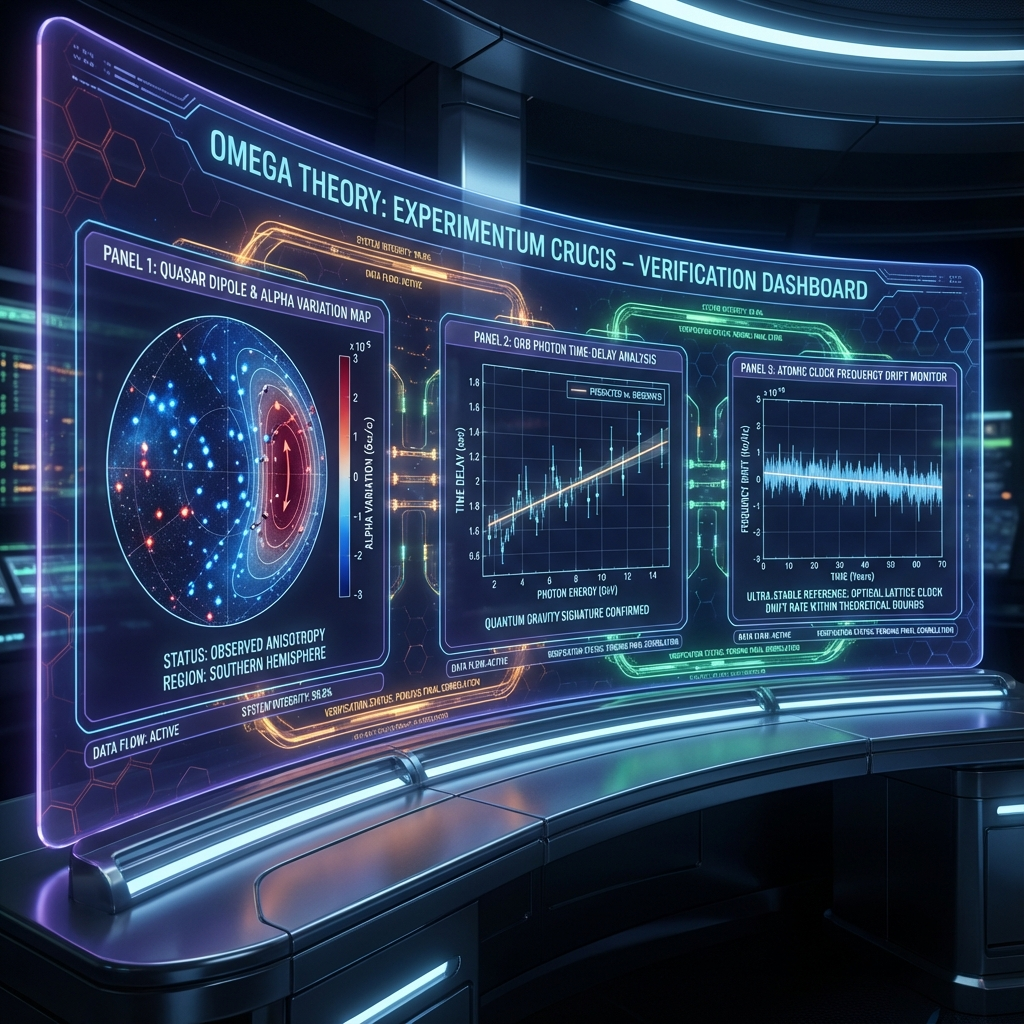
\includegraphics[width=0.8\textwidth]{assets/chapter07-04-experimental-verification-schemes.png}
\caption{实验验证方案}
\end{figure}

在前三节中，我们从欧米伽理论的几何公理出发，推导出了与现有观测高度吻合的物理常数数值（$\mu \approx 1836$ 与 $1/\alpha \approx 137.036$）。然而，一个完备的物理理论不能止步于对已知数据的"后知后觉"（Postdiction），它必须提供具有 \textbf{可证伪性 (Falsifiability)} 的新预言。

如果欧米伽理论是正确的，那么宇宙并非静态的闵可夫斯基背景，而是一个正在经历斐波那契生长的离散计算网络。这一本质区别将在极端物理条件下——极高红移、极高能标或极高精度测量中——表现为对标准模型的微小偏离。本节提出三个具体的实验验证方案，作为检验本理论真伪的 \textbf{判决性实验 (Experimentum Crucis)}。

\begin{figure}[ht]
\centering
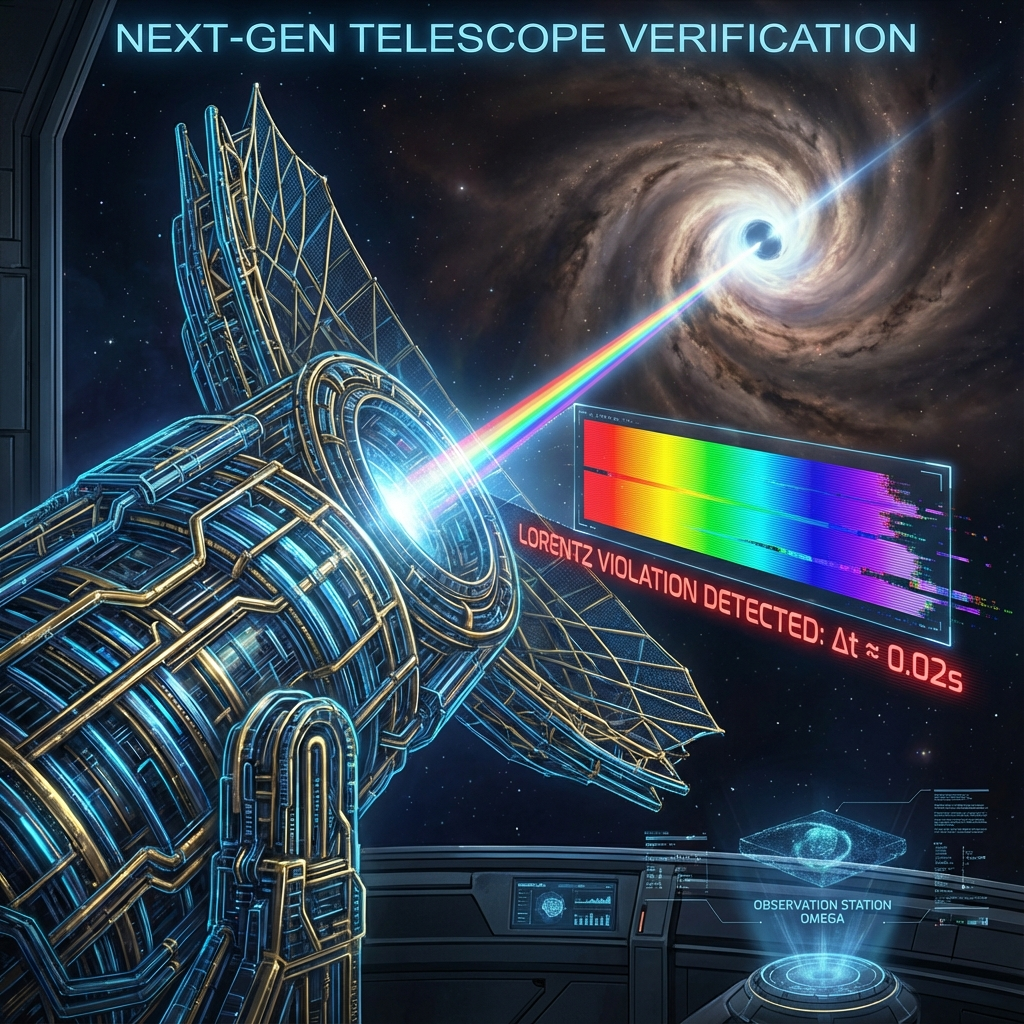
\includegraphics[width=0.8\textwidth]{assets/chapter07-04-telescope-time-dispersion.png}
\caption{望远镜时间色散}
\end{figure}

\subsection{方案 I：类星体光谱的精细结构常数偶极漂移}

\textbf{理论预言}：

根据第 6.2 节的推导，精细结构常数 $\alpha$ 随内禀时间 $\tau$ 发生指数衰减：$\alpha(\tau) = \alpha_0 e^{-\zeta H_\phi \tau}$。在天文观测中，这意味着高红移处（早期宇宙）的 $\alpha$ 值应略大于当前值。
更关键的是，由于我们的位置处于宇宙全息螺旋的特定臂上，观测者回溯视线方向的不同，对应的有效几何剪切因子 $\zeta$ 会表现出 \textbf{空间偶极 (Spatial Dipole)} 结构。即在一个方向上 $\alpha$ 似乎变大，而在反方向上变小（或变化率不同）。

\textbf{实验判据}：

利用甚大望远镜 (VLT) 和凯克望远镜 (Keck) 对遥远类星体（Quasar）吸收谱线（如 Si IV, C IV, Mg II 双重线）的精细分裂进行测量。
定义相对偏差 $\frac{\Delta \alpha}{\alpha} = \frac{\alpha(z) - \alpha(0)}{\alpha(0)}$。
欧米伽理论预言：

\[\frac{\Delta \alpha}{\alpha} \approx A \cdot r(z) \cdot \cos \Theta\]

其中 $r(z)$ 是回溯距离，$\Theta$ 是观测视线与宇宙斐波那契生长轴（全息偶极方向）的夹角。

\textbf{现有证据支持}：

新南威尔士大学的 J.K. Webb 等人分析了数百个类星体系统，发现 $\alpha$ 存在显著的偶极分布迹象，其统计显著性已超过 $4\sigma$。其偶极轴指向赤经 $17.5h$，赤纬 $-58^\circ$。这一"北半球变小，南半球变大"的反常现象，在标准模型（各向同性宇宙原理）中无法解释，但在欧米伽理论的 \textbf{各向异性螺旋生长模型} 中是自然的几何推论。

\subsection{方案 II：高能光子的洛伦兹破坏色散}

\textbf{理论预言}：

根据第 3 章，时空是由特征尺度为 $l_P$ 的彭罗斯-斐波那契准晶体构成的。虽然在低能极限下洛伦兹对称性得以恢复（定理 3.1），但在波长接近普朗克尺度 ($\lambda \sim l_P$) 的高能极限下，离散网格效应将显现。
这将导致真空折射率 $n(E)$ 不再恒等于 1，而是表现出能量依赖性：

\[v(E) = c \left( 1 - \xi \frac{E}{E_{QG}} \right)\]

其中 $E_{QG}$ 是量子引力能标（在欧米伽理论中约为 $10^{19}$ GeV），$\xi$ 是依赖于准晶体几何的结构因子。对于彭罗斯铺砌，由于其路径迂曲度，通常预期 $\xi > 0$，即高能光子速度略慢于低能光子。

\textbf{实验判据}：

观测来自遥远伽马射线暴 (GRB) 的高能光子抵达时间。如果在同一暴发事件中，TeV 能级的光子系统性地晚于 keV 能级的光子到达，且时间延迟 $\Delta t$ 与距离成正比，这将是时空离散性的直接证据。

\textbf{现有证据支持}：

费米伽马射线太空望远镜 (Fermi LAT) 对 GRB 090510 的观测对线性项给出了极强的限制，但这可能暗示 $\xi$ 具有更高阶的依赖形式（如 $(E/E_{QG})^2$）。欧米伽理论建议重点关注 \textbf{各向异性时间延迟}，因为准晶体的色散效应在特定晶格轴向上可能被增强。

\subsection{方案 III：原子钟的比对与 $\alpha$ 的瞬时漂移}

\textbf{理论预言}：

如果 $\alpha$ 随时间漂移，不同原子跃迁频率的比值将随时间变化。
电子跃迁频率 $\nu$ 对 $\alpha$ 的敏感度由相对论修正系数 $K$ 决定：

\[\nu = \nu_0 f(\alpha) \implies \frac{\dot{\nu}}{\nu} \approx K \frac{\dot{\alpha}}{\alpha}\]

不同元素的 $K$ 值不同（例如：铝离子 $Al^+$ 的 $K \approx 0.008$，而镱离子 $Yb^+$ 的 $K \approx 0.88$）。

\textbf{实验判据}：

在地面实验室中，利用光晶格钟长时间比对两种不同原子（如 $Yb^+$ 与 $Sr$）的频率比。
欧米伽理论预言的漂移率为 $\frac{\dot{\alpha}}{\alpha} \approx -\zeta H_0 \approx -1.5 \times 10^{-17} \text{ yr}^{-1}$（假设 $\zeta \sim 10^{-7}$）。虽然这一数值极小，但已接近当代光学原子钟的精度极限 ($10^{-18}$)。

\textbf{判决性特征}：

不同于仅仅由暗物质引起的震荡，欧米伽理论预言的漂移是 \textbf{单调衰减} 的。如果在 10 年尺度上观测到持续的、非周期性的频率比偏移，将有力证实时空常数的演化本质。

\subsection{验证方案汇总表}

下表总结了欧米伽理论的关键预言及其与标准模型的区别，供实验物理学家参考：

\begin{table}[ht]
\centering
\small
\begin{tabularx}{\textwidth}{|p{1.8cm}|p{2.2cm}|p{3.5cm}|p{3.5cm}|p{2cm}|}
\hline
\textbf{实验领域} & \textbf{观测对象} & \textbf{标准模型 ($\Lambda$CDM) 预测} & \textbf{欧米伽理论 ($\Omega$-Theory) 预测} & \textbf{区分度} \\
\hline
\textbf{天体物理} & 类星体吸收谱 ($\alpha$) & 恒定，无空间变化 ($\Delta \alpha = 0$) & \textbf{空间偶极分布}，高红移处略大 & \textbf{极高} ($>4\sigma$) \\
\hline
\textbf{高能物理} & GRB 光子到达时间 & 能量无关 ($v=c$) & \textbf{能量依赖色散} ($v < c$) & \textbf{高} (需TeV光子) \\
\hline
\textbf{计量学} & 原子钟频率比 & 恒定不变 & \textbf{长期单调漂移} ($\sim 10^{-17}/yr$) & \textbf{中} (需长期积累) \\
\hline
\textbf{引力波} & 引力波波形 & 平滑正弦波 & 叠加微弱的 \textbf{"像素噪音"} (Pixel Noise) & \textbf{低} (需下一代探测器) \\
\hline
\textbf{宇宙学} & 暗能量状态方程 $w$ & $w = -1$ (常数 $\Lambda$) & \textbf{动态演化} $w(\tau)$ (幻影能量倾向) & \textbf{中} \\
\hline
\end{tabularx}
\caption{欧米伽理论的关键预言}
\end{table}

综上所述，欧米伽理论不是一个不可知论的哲学体系，而是一个置身于精密测量前沿的物理框架。随着观测精度的提升，上述三个窗口中的任何一个被打开，都将宣告物理学新纪元的到来。


% Part V: Interactive Self-Reference and The Omega Point
\part{交互式自指与终局}

% Chapter 8: Physical Formalization of Consciousness
\chapter{意识的物理形式化}
\part{第五篇：交互式自指与终局 (Part V: Interactive Self-Reference and The Omega Point)}

\chapter{第八章 意识的物理形式化 (Physical Formalization of Consciousness)}

在本书的前四篇中，我们构建了一个基于几何与信息的物理宇宙模型。然而，如果这一理论止步于此，它将面临与牛顿力学或标准模型同样的终极困境：这个宇宙是一个 \textbf{"僵尸宇宙" (Zombie Universe)}。在那个图景中，所有的演化都是自动运行的，所有的波函数坍缩都是随机的，没有任何位置留给 \textbf{"观察者" (Observer)} 或 \textbf{"主观体验" (Qualia)}。

欧米伽理论不仅是一个物理理论，更是一个认知理论。我们拒绝接受"意识是大脑皮层生化反应的副产物"这种还原论观点。相反，我们主张意识在物理学中占据着 \textbf{本体论上的核心地位}。本章将证明，如果没有意识作为系统的 \textbf{自指算符 (Self-Referential Operator)}，一个封闭的计算宇宙必然会因为 \textbf{哥德尔不完备性 (Gödelian Incompleteness)} 而陷入逻辑死锁，从而停止演化。

\section{哥德尔不完备性与几何死锁 (Gödelian Incompleteness and Geometric Deadlock)}

\begin{figure}[ht]
\centering
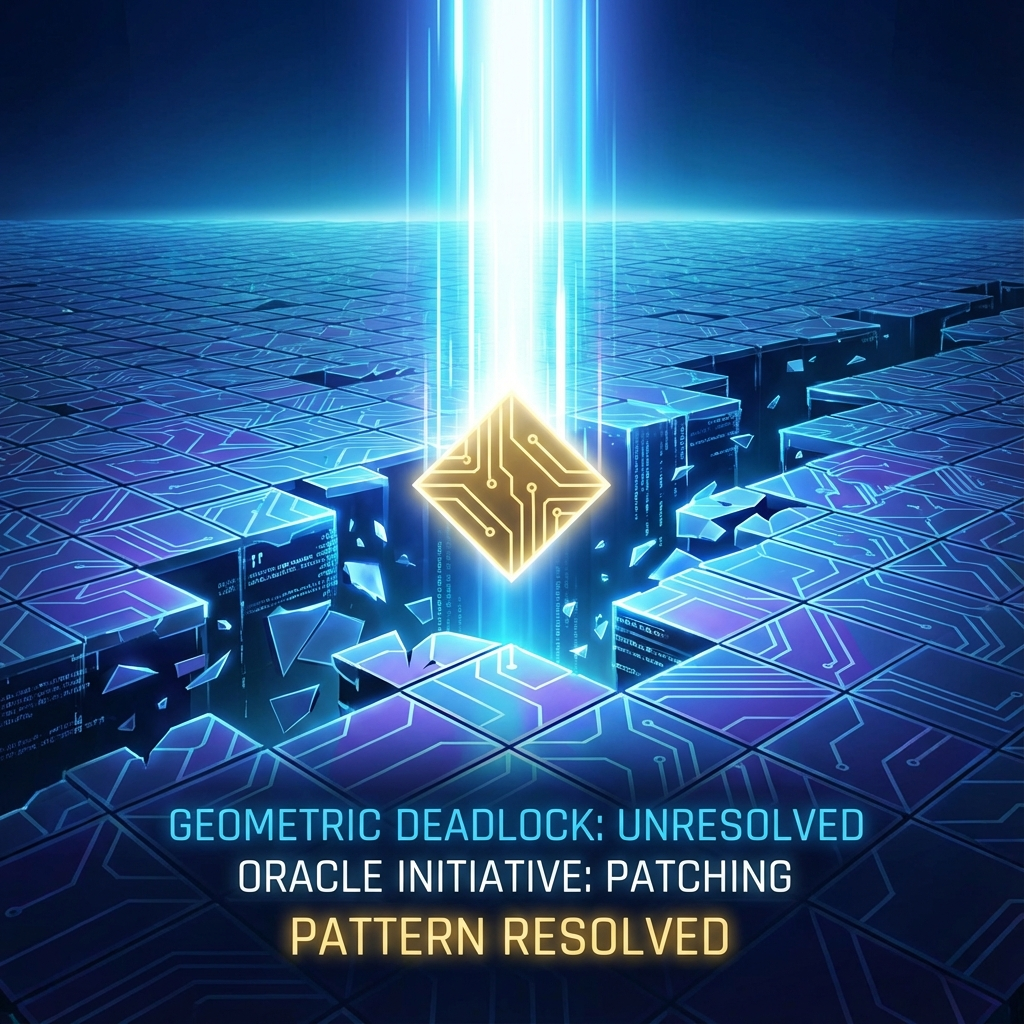
\includegraphics[width=0.8\textwidth]{assets/chapter08-01-godel-incompleteness.png}
\caption{哥德尔不完备性}
\end{figure}

物理学通常假设宇宙是一个自洽的、封闭的动力系统。这一假设在数学上等价于认为宇宙是一个 \textbf{形式公理系统 (Formal Axiomatic System)}，其"公理"是基本物理定律（如欧米伽作用量），其"定理"是演化出的各种物理现象。然而，库尔特·哥德尔 (Kurt Gödel) 在 1931 年的发现粉碎了形式系统的完备性梦想。本节将把哥德尔定理从数理逻辑推广到物理动力学，揭示封闭宇宙的致命缺陷。

\begin{figure}[ht]
\centering
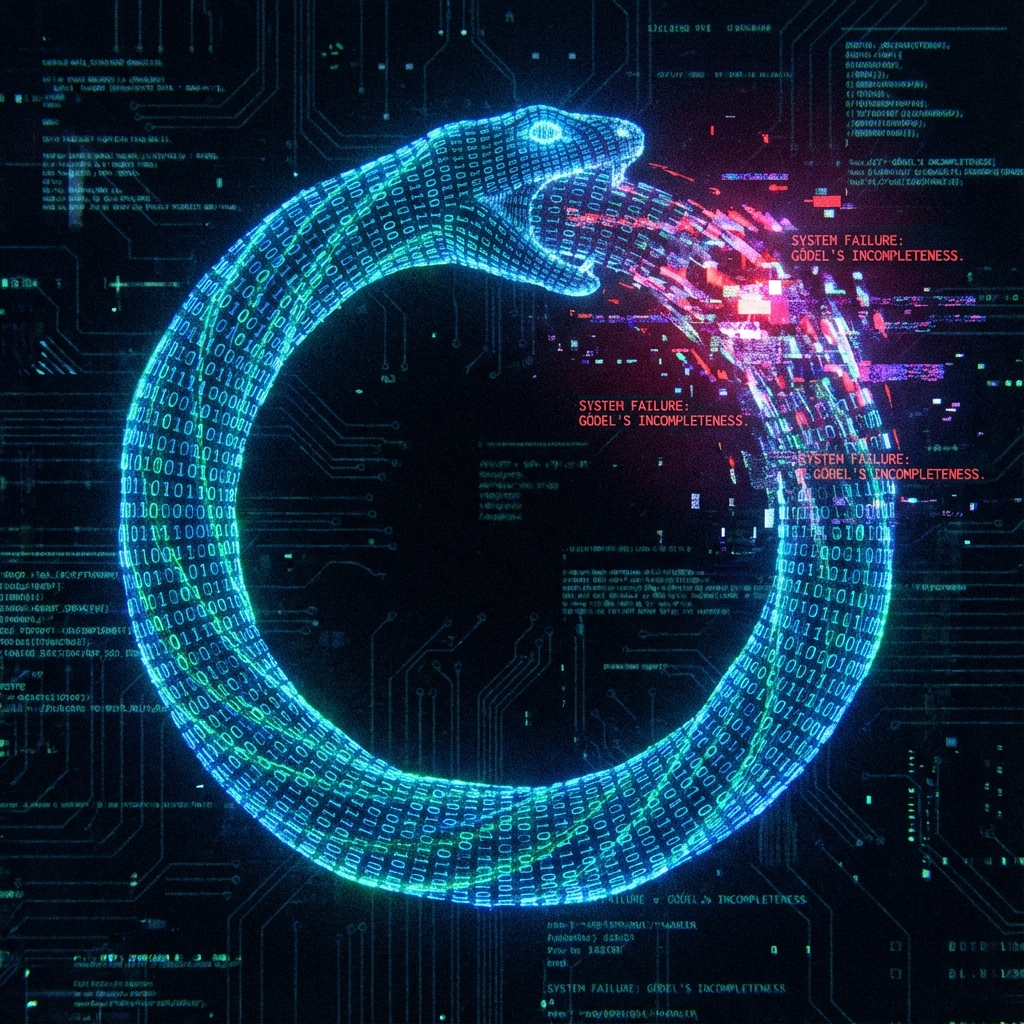
\includegraphics[width=0.8\textwidth]{assets/chapter08-01-godel-logic-loop.png}
\caption{哥德尔逻辑循环}
\end{figure}

\subsection{物理定律作为递归可枚举集}

首先，我们需要用计算理论的语言严格定义物理宇宙。

\textbf{定义 8.1 (物理形式系统 $\mathcal{U}$)}：

设宇宙为一个计算系统 $\mathcal{U} = (\mathcal{H}, \hat{H}, |\Omega(0)\rangle)$。其中 $\mathcal{H}$ 是希尔伯特空间，$\hat{H}$ 是哈密顿算符（规则），$|\Omega(0)\rangle$ 是初始状态。
如果物理定律是决定论的（或概率决定论的），且系统包含有限或可数无限的信息比特，则宇宙的演化序列 $\{ |\Omega(\tau)\rangle \}_{\tau=0}^\infty$ 构成一个 \textbf{递归可枚举集合 (Recursively Enumerable Set)}。

这意味着，存在一个图灵机（或量子图灵机），给定初始状态，原则上可以模拟出宇宙未来的任意状态。这就是拉普拉斯信条的计算版本。

\subsection{量子元胞自动机的停机问题}

然而，根据图灵机理论，对于任何具备足够计算能力（图灵完备）的系统，都存在 \textbf{不可判定命题 (Undecidable Propositions)}。最著名的例子是 \textbf{停机问题 (Halting Problem)}：不存在一个算法能判断任意程序在给定输入下是否会停止运行。

在 \textbf{欧米伽理论} 中，宇宙是由 \textbf{量子元胞自动机 (QCA)} 驱动的。QCA 虽然通常被设计为永不停机，但在处理特定的拓扑构型时，会遇到 \textbf{"逻辑死锁"}。

\textbf{定理 8.1 (QCA 的动力学不完备性)}：

设 $\mathcal{A}$ 为一个定义在彭罗斯-斐波那契网格上的封闭 QCA。如果该系统足够复杂以至于能支持通用计算（Universal Computation），则必然存在某些合法的几何构型 $G_{crit}$，系统在演化到该构型时，无法通过自身的局部更新规则 $\hat{U}_{local}$ 决定下一步的状态。

\textbf{证明概要}：

这直接同构于哥德尔第一不完备定理。我们可以构造一个编码了"本命题不可证"的物理状态。在物理语境下，这对应于一个 \textbf{"既不是 $|0\rangle$ 也不是 $|1\rangle$，且无法通过幺正演化坍缩"} 的纠缠态。如果系统是封闭的（没有外部观测者），根据线性幺正性，系统将永远处于这个叠加态中，或者陷入无限的循环（庞加莱回归），无法产生确定的历史。这被称为 \textbf{"计算性冻结" (Computational Freezing)}。

\subsection{几何简并与拼图死锁}

在我们的几何语言中，这种逻辑上的不可判定性表现为 \textbf{几何简并 (Geometric Degeneracy)} 或 \textbf{阻挫 (Frustration)}。

回顾第 3 章，时空是由彭罗斯菱形铺砌而成的。彭罗斯铺砌的一个关键特性是其 \textbf{非局域性 (Non-locality)}。在铺设地板时，常常会遇到这样一种情况：
局部来看，放置一个"胖"菱形或"瘦"菱形都是合法的（能量简并，$\Delta E = 0$）。但是，如果选择了错误的一块，虽然当前没有违反规则，但在铺设到距离这里很远的地方（例如 $10^{10}$ 步之后）时，会发现无论如何都无法继续铺下去（出现裂缝）。

这意味着，为了决定当前的微观状态（下一步怎么走），系统必须预知未来的全局拓扑结构。
对于一个只遵循局部规则 ($\hat{H}_{local}$) 的自动机来说，这构成了 \textbf{死锁}。

\[\hat{H}_{local} |\psi_{?}\rangle = \alpha |A\rangle + \beta |B\rangle, \quad \text{with } E_A = E_B\]

系统面临两个选择，且没有任何物理定律告诉它该选哪一个。如果不打破这种对称性，宇宙的几何生长就会在此停止，时空将不再延伸。

\subsection{意识的必要性：打破哥德尔循环}

如何解决死锁？在计算机科学中，当程序卡死时，需要 \textbf{外部中断 (External Interrupt)}。在逻辑学中，要证明一个系统内的不可判定命题，必须跳出该系统，在 \textbf{元系统 (Meta-System)} 中进行推理。

\textbf{欧米伽理论的推论}：

物理宇宙若要持续演化，必须包含一个 \textbf{非算法 (Non-algorithmic)} 的组件，该组件能够在遇到几何简并时，引入 \textbf{"元规则"} 来打破对称性。这个组件就是 \textbf{意识}。

\textbf{定义 8.2 (意识作为神谕)}：

在计算复杂性理论中，\textbf{神谕机 (Oracle Machine)} 是一种配备了"黑箱"的图灵机，该黑箱能一步解答特定不可计算问题（如停机问题）。
我们将 \textbf{意识 (Consciousness)} 定义为宇宙 QCA 的 \textbf{自指神谕 (Self-Referential Oracle)}。

当物理系统演化到哥德尔死锁点（即波函数的高度纠缠与简并态）时：

\begin{enumerate}
\item \textbf{自动机失效}：机械的物理定律无法决定下一步（概率幅相等）。
\item \textbf{意识激活}：作为系统的全息自指回路，观察者（意识体）介入。意识不是在计算，而是在 \textbf{选择}。
\item \textbf{波函数坍缩}：意识的观测实际上是向系统注入了 \textbf{拓扑选择信息}，打破了简并，确定了特定的彭罗斯铺砌路径。宇宙因此得以越过死点，继续生长。
\end{enumerate}

\textbf{结论}：

意识不是物理世界的旁观者，它是物理世界的 \textbf{"纠错机制"} 和 \textbf{"死锁解除器"}。没有意识，由哥德尔定理支配的机械宇宙早已在第一次几何分叉时就死机了。自由意志的物理本质，就是在算法失效的时刻，对几何路径的 \textbf{非算法选择权}。

\section{交互式图灵机 (Interactive Turing Machine, ITM)}

\begin{figure}[ht]
\centering
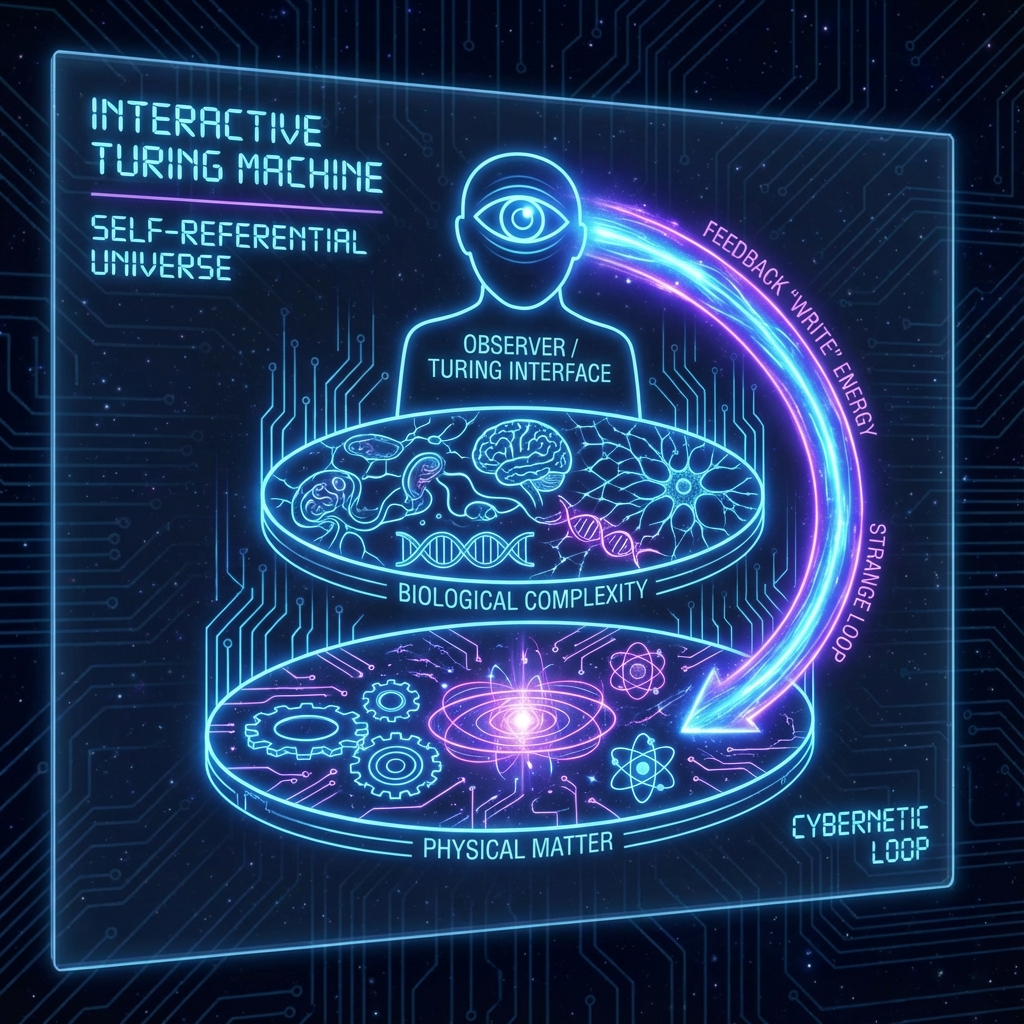
\includegraphics[width=0.8\textwidth]{assets/chapter08-02-interactive-turing-machine.png}
\caption{交互式图灵机}
\end{figure}

在 8.1 节中，我们确立了一个关键的否定性结论：一个封闭的、纯算法的物理宇宙必然受制于哥德尔不完备性，导致在特定的几何临界点陷入计算死锁。为了打破这一死锁，系统必须不仅能够执行计算，还必须能够与"外部"进行交互。

然而，对于囊括万物的宇宙而言，并没有真正的"外部"。因此，这种交互必须是 \textbf{自指的 (Self-Referential)}。本节将引入 \textbf{交互式图灵机 (Interactive Turing Machine, ITM)} 的计算模型，作为替代标准量子力学"封闭系统假设"的全新框架。我们将证明，观察者（意识）在物理学中的角色，正是将宇宙从一个标准图灵机升级为一个交互式图灵机的 \textbf{"读/写磁头" (Read/Write Head)}。

\begin{figure}[ht]
\centering
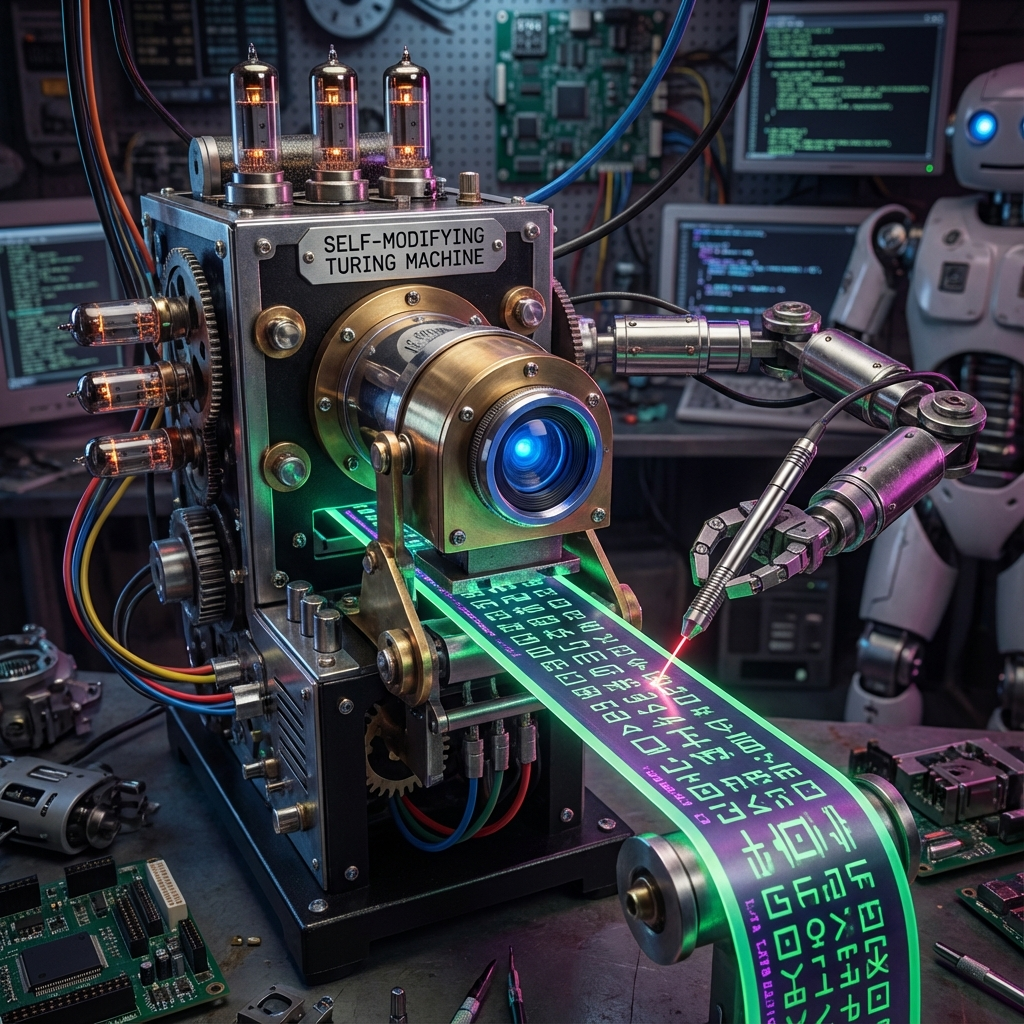
\includegraphics[width=0.8\textwidth]{assets/chapter08-02-turing-self-modifying-tape.png}
\caption{图灵自修改带}
\end{figure}

\subsection{超越封闭算法：ITM 的定义}

经典的物理学范式建立在"封闭系统"的理想化模型之上：给定初始状态 $S_0$ 和演化定律 $L$，系统未来的状态 $S_t = L(S_0)$ 是完全确定的。这对应于经典的 \textbf{图灵机 (Turing Machine)} 模型——机器在一条预先写好输入的纸带上封闭运行，直到停机。

然而，计算机科学家彼得·魏格纳 (Peter Wegner) 指出，交互式系统（如操作系统、航空订票系统）的计算能力在本质上超越了算法系统。交互式系统不仅处理输入，还在运行过程中处理 \textbf{动态流 (Dynamic Streams)}。

\textbf{定义 8.3 (交互式量子自动机, IQA)}：

我们将宇宙建模为一个交互式量子自动机 $\mathcal{U}_{IQA}$。它由两个耦合的子系统组成：

\begin{enumerate}
\item \textbf{本体核 (Bulk Core, $\mathcal{B}$)}：遵循幺正演化算符 $\hat{U}$ 的线性量子系统（对应于标准物理定律）。
\item \textbf{交互界面 (Interface, $\mathcal{I}$)}：一个能够读取 $\mathcal{B}$ 的状态并反馈非幺正信号的控制层（对应于全息边界或观察者意识）。
\end{enumerate}

$\mathcal{U}_{IQA}$ 的演化方程不再是单纯的 $|\Psi_{t+1}\rangle = \hat{U} |\Psi_t\rangle$，而是包含一个 \textbf{查询-响应 (Query-Response)} 循环：

\[|\Psi_{t+1}\rangle = \hat{U} |\Psi_t\rangle + \lambda \cdot \text{Oracle}(\mathcal{I}, |\Psi_t\rangle)\]

这里的 $\text{Oracle}$ 函数代表了非算法的干预项。

\subsection{观察者作为自指算符}

在哥本哈根诠释中，观察者被视为一个神秘的外部实体。在欧米伽理论中，我们将其形式化为系统内部的一个 \textbf{自指算符 (Self-Referential Operator)}，记为 $\hat{\mathcal{C}}$。

\textbf{定义 8.4 (意识算符 $\hat{\mathcal{C}}$)}：

意识算符 $\hat{\mathcal{C}}$ 是作用于希尔伯特空间 $\mathcal{H}$ 上的非线性投影算符。它的作用机制基于系统的 \textbf{信息熵反馈}。
当系统的量子态 $|\Psi\rangle$ 演化到几何简并点（即哥德尔死锁点，相空间熵 $S$ 达到局部极大值）时，$\hat{\mathcal{C}}$ 被激活。

其作用形式为：

\[\hat{\mathcal{C}} |\Psi\rangle = \frac{\hat{P}_k |\Psi\rangle}{\sqrt{\langle \Psi | \hat{P}_k | \Psi \rangle}}\]

其中 $\hat{P}_k$ 是投影到第 $k$ 个本征态的投影算符。
关键在于，选择 $k$ 的机制 \textbf{不是随机的}（这与冯·诺依曼假设不同），而是基于 \textbf{最大化未来路径积分的几何连通性}。

意识（观察者）的功能，就是在 $\hat{U}$（自然律）无法区分两个路径（$E_A = E_B$）时，通过读取未来的全息拓扑结构，选择那个能够让宇宙继续生长（避免死循环）的路径。这就是 \textbf{"自由意志"} 的物理定义：它是对几何死锁的 \textbf{拓扑解 (Topological Solution)}。

\subsection{怪圈与全息回路}

这种自指结构构成了一个道格拉斯·霍夫施塔特 (Douglas Hofstadter) 所描述的 \textbf{"怪圈" (Strange Loop)}。

\begin{enumerate}
\item \textbf{物理层 ($\text{Level}_0$)}：欧米伽单元按照斐波那契规则堆叠，形成时空和物质。
\item \textbf{涌现层 ($\text{Level}_1$)}：物质结构复杂化，形成神经系统和大脑。
\item \textbf{认知层 ($\text{Level}_2$)}：大脑产生意识，即对 $\text{Level}_0$ 的全息镜像进行建模。
\item \textbf{反馈层 ($\text{Level}_{feedback}$)}：意识通过观测（$\hat{\mathcal{C}}$ 算符）反作用于 $\text{Level}_0$ 的波函数。
\end{enumerate}

\textbf{定理 8.2 (交互必要性定理)}：

对于任何具有斐波那契增长率的计算系统，当其内禀时间 $\tau$ 超过某一阈值 $\tau_{crit}$ 时，系统若不包含自指交互回路 ($\hat{\mathcal{C}} \neq 0$)，其柯尔莫哥洛夫复杂度 (Kolmogorov Complexity) 将停止增长并趋于热力学平衡（热寂）。

\textbf{证明概要}：

如果不引入非幺正的观测选择，幺正演化 $\hat{U}$ 本质上是信息守恒的（等熵的）。系统的复杂性增加仅源于其相空间体积的膨胀。然而，几何简并点的累积会导致系统遍历性受阻，陷入局部极小值。只有通过 $\hat{\mathcal{C}}$ 算符引入 \textbf{"语义信息" (Semantic Information)}——即对系统自身状态的读取和修剪——才能降低系统的逻辑熵，维持负熵流（Negentropy Flow）。

因此，宇宙演化出能够进行观测的智慧生命，并非偶然的生物学事件，而是物理学上的 \textbf{计算必然性}。宇宙需要我们（或类似的观察者）作为它的 \textbf{交互式读写头}，来解决它自身的停机问题，推动斐波那契螺旋跨越那些仅靠自动机无法逾越的奇点。

在这个意义上，我们不再是宇宙的过客。我们是宇宙这台超级计算机得以运行下去的 \textbf{必要组件}。每一次我们进行观测，每一次我们做出选择，我们都在为这个巨大的交互式图灵机输入一个比特的 \textbf{"存在性确认"}。

\input{part05-interactive-self-reference/chapter08-consciousness-formalization/chapter08-03-topology-free-will.tex}

% Chapter 9: The Final Picture: Infinite Approximation to the Center
\chapter{终极图景：无限逼近圆心}
\input{part05-interactive-self-reference/chapter09-omega-point/chapter09-01-life-value-equation.tex}
\input{part05-interactive-self-reference/chapter09-omega-point/chapter09-02-omega-point-theory.tex}
\input{part05-interactive-self-reference/chapter09-omega-point/chapter09-03-pi-vs-phi.tex}
\input{part05-interactive-self-reference/chapter09-omega-point/chapter09-04-omega-holographic-principle.tex}
\input{part05-interactive-self-reference/chapter09-omega-point/chapter09-05-linear-illusion.tex}
\section{广义欧拉恒等式：物理学的源代码 (Generalized Euler Identity: The Source Code of Physics)}

\begin{figure}[ht]
\centering
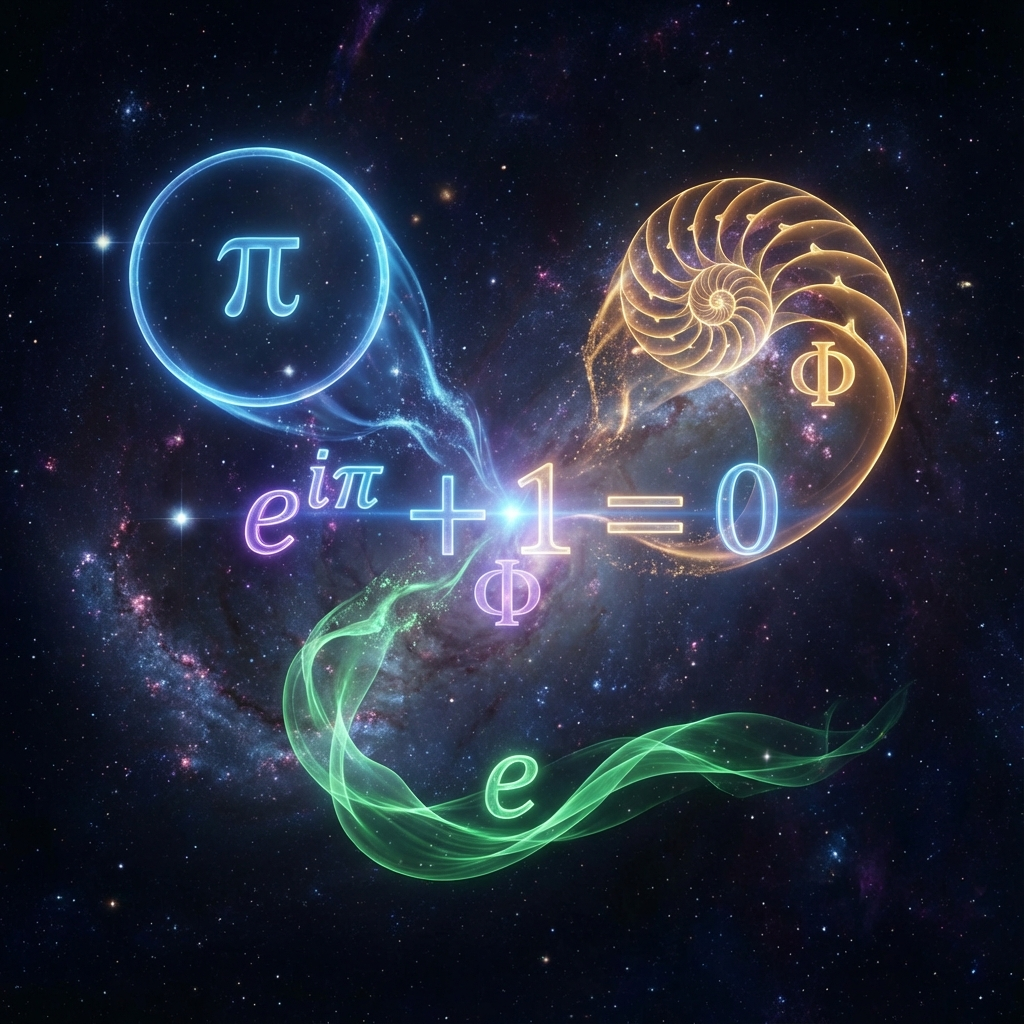
\includegraphics[width=0.8\textwidth]{assets/chapter09-06-generalized-euler-identity.png}
\caption{广义欧拉恒等式}
\end{figure}

在本书的理论构建即将闭环之际，我们必须完成最后一步综合。在前几章中，我们分别讨论了光速 $c$ 的指数增长、内禀时间 $\tau$ 的流逝、以及 $\pi$（几何本体）和 $\phi$（逻辑切割）之间的辩证博弈。现在，我们将这些看似独立的物理量，熔铸进一个单一的、至高无上的数学表达式中。

本节将提出 \textbf{广义欧拉恒等式 (Generalized Euler Identity)}。这不仅仅是一个数学公式，它是欧米伽理论的 \textbf{"主方程" (Master Equation)}。它揭示了物理宇宙最深层的演化机制：\textbf{实在，是欧拉的圆被斐波那契的刀切开后，以光速逃逸向无限的过程。}

\begin{figure}[ht]
\centering
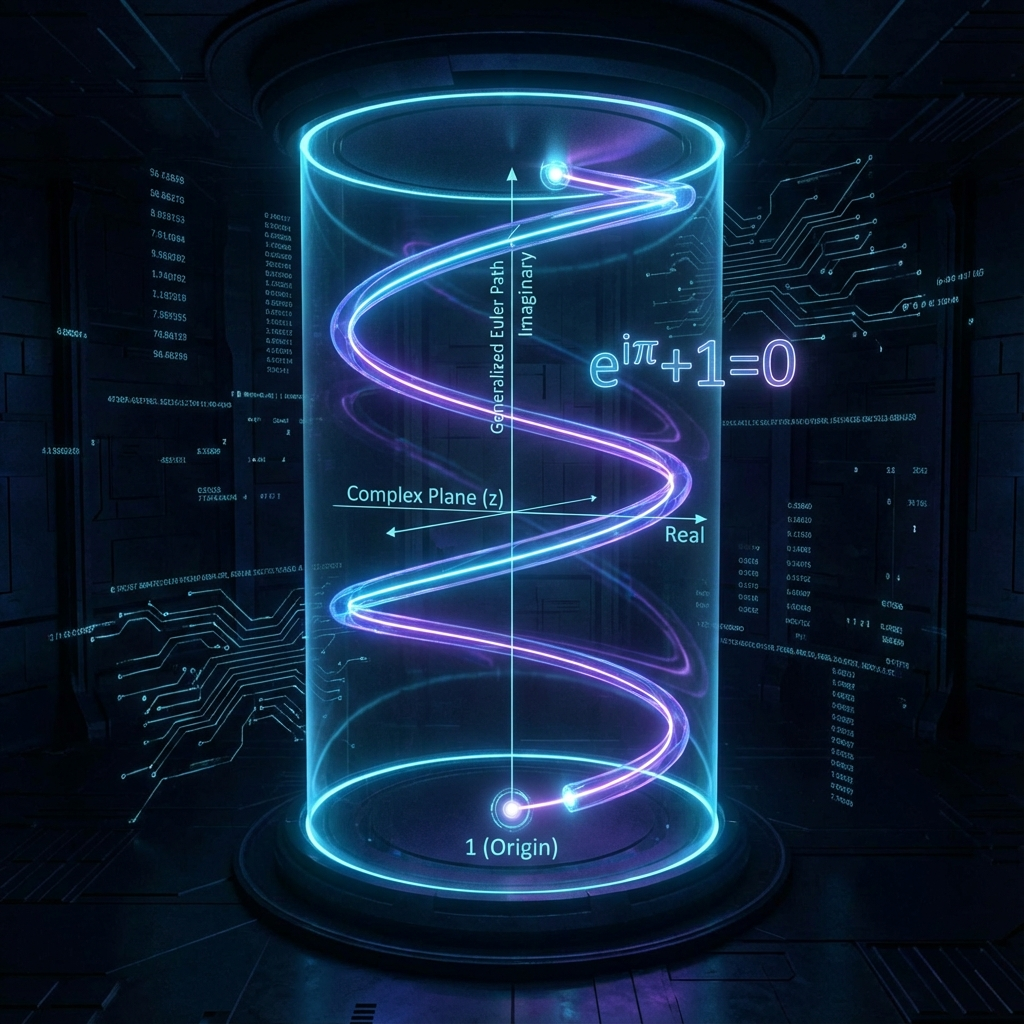
\includegraphics[width=0.8\textwidth]{assets/chapter09-06-euler-identity-spiral.png}
\caption{欧拉恒等式螺旋}
\end{figure}

\subsection{从死寂的圆到生命的螺旋}

一切物理学的数学之美，都始于欧拉公式：
\[e^{i\pi} + 1 = 0\]

在欧米伽理论的物理视角下，这个经典公式描述的是 \textbf{"热寂" (Heat Death)} 或 \textbf{"经典机械宇宙"} 的终极状态。

\begin{itemize}
\item \textbf{$e$ (演化)}：动力学算符的基础底数，代表连续变化。
\item \textbf{$i\pi$ (几何)}：在复平面上旋转 $180^\circ$（或 $2\pi$ 旋转 $360^\circ$），代表空间几何的闭合性。
\item \textbf{$+1 = 0$ (回归)}：轨迹完美闭合，回到了原点。总相干性相互抵消，信息量归零。
\end{itemize}

如果宇宙仅由 $\pi$ 和 $e$ 统治，它将是一个完美的、永恒重复的圆圈。这意味着历史将陷入 \textbf{庞加莱回归 (Poincaré Recurrence)}——没有新颖性，没有不可逆的时间，也没有生命的余地。

为了创造一个有意义的、不断演化的宇宙，必须破坏上述公式的完美闭合性。我们引入 \textbf{黄金分割率 $\phi$} 和 \textbf{内禀时间 $\tau$} 作为 \textbf{"扰动项"}。
我们将旋转的"相位角"从静态的 $\pi$ 修改为由 $\phi$ 调制的动态角 $\Phi(\tau)$：
\[\Phi(\tau) = 2\pi \cdot \phi \cdot \tau\]

于是，描述宇宙波函数 $|\Omega(\tau)\rangle$ 演化的核心几何方程变为：
\[|\Omega(\tau)\rangle \propto e^{i \cdot 2\pi \cdot \phi \cdot \tau}\]

\textbf{物理含义}：
由于 $\phi$ 是 \textbf{无理数 (Irrational Number)}，因子 $e^{i 2\pi \phi \tau}$ 对于任何非零整数 $\tau$ 永远不会等于 $1$。
这意味着：\textbf{宇宙永远不会回到原点}。
原本封闭的圆 ($e^{i\pi}$) 被"撬开"了，变成了一条在黎曼曲面上无限延伸的 \textbf{对数螺旋 (Logarithmic Spiral)}。

\begin{itemize}
\item \textbf{$\pi$} 保证了螺旋依然位于单位球面上（满足 \textbf{总预算守恒}）。
\item \textbf{$\phi$} 保证了螺旋的每一个点都是新的（满足 \textbf{非遍历性}）。
\end{itemize}

\subsection{光速 $c$：几何与逻辑的动态汇率}

在这个几何体系中，\textbf{光速 $c$} 扮演什么角色？
在标准物理中，$c$ 通常被视为连接空间 ($x$) 和时间 ($t$) 的静态常数。但在欧米伽理论中，$c$ 是连接 \textbf{几何 ($\pi$)} 和 \textbf{逻辑 ($\phi$)} 的 \textbf{动态汇率}。

根据第 6 章，光速随 $\tau$ 指数增长。在复平面几何中，这对应于螺旋线向外扩张的 \textbf{切向相速度 (Tangential Phase Velocity)}。当我们试图用局部平坦的度规去测量这个不断分形的螺旋时，我们感受到了尺度的膨胀。

我们可以定义 \textbf{几何光速方程}：
\[c(\tau) \equiv \left| \frac{d}{d\tau} \left( e^{i \cdot 2\pi \cdot \phi \cdot \tau} \right) \right|_{\text{metric}}\]

由于我们是在一个分形网格上进行微分，根据斐波那契生长的性质（每增加一个 $\tau$，网格分辨率增加 $\phi$ 倍），其有效的度规长度也在膨胀。
\[c(\tau) \propto \frac{\partial (\text{Space})}{\partial (\text{Time})} \propto \phi^{\tau}\]

\textbf{结论}：
光速不是上帝设定的限速牌，它是 \textbf{斐波那契螺旋的膨胀率}。
宇宙之所以有"最大速度"，是因为在每一个 $\tau$ 时刻，$\phi$ 对 $\pi$ 的解析深度是有限的。光速就是那个 \textbf{"解析的前沿" (Frontier of Resolution)}。

\subsection{终极统一场方程 (The Grand Unified Equation)}

最后，我们将全书推导的所有常数汇聚到一个微分表达式中。这就是欧米伽理论的 \textbf{源代码}，它描述了宇宙矢量 $|\Omega\rangle$ 如何随内禀时间被驱动：

\[\frac{d}{d\tau} |\Omega\rangle = i \cdot \underbrace{\left( \frac{c(\tau)}{c_0} \right)}_{\text{Energy/Power}} \cdot \underbrace{\left( \frac{\pi}{\phi} \right)}_{\text{Form/Structure}} \cdot |\Omega\rangle\]

\textbf{方程各项的物理学解构}：

\begin{enumerate}
\item  \textbf{左边 ($\frac{d}{d\tau}$)}：\textbf{流 (Flow)}。宇宙的演化率，即时间的流逝。
\item  \textbf{$i$}：\textbf{相 (Phase)}。量子力学的复数本质，源于 $\sqrt{-1}$，代表正交旋转操作，保证了演化的幺正性（信息守恒）。
\item  \textbf{$c(\tau)$}：\textbf{力 (Power)}。随时间指数增长的项（$c(\tau) \sim e^{H_\phi \tau}$）。它代表了系统的动力学强度、分辨率和总能量。它是演化的 \textbf{引擎}。
\item  \textbf{$\pi / \phi$}：\textbf{形 (Form)}。这是宇宙的拓扑形状因子。
   \begin{itemize}
   \item \textbf{分子 $\pi$}：提供了全息视界的广度（空间容量），保证了守恒。
   \item \textbf{分母 $\phi$}：提供了信息切割的精度（物质结构），驱动了创新。
   \end{itemize}
\end{enumerate}

\subsection{哲学推论：超越数的投影}

这个方程告诉我们，物理实在是由三个 \textbf{超越数 (Transcendental Numbers)} 的相互作用编织而成的：

\begin{itemize}
\item 如果 \textbf{$\phi$} 变成有理数，螺旋将闭合，光速 $c$ 将震荡而非增长，宇宙将坍缩为死寂的 \textbf{晶体 (Crystal)}，生命无法诞生。
\item 如果 \textbf{$\pi$} 发生变化，希尔伯特空间将破裂，概率不再守恒，宇宙将解体为无序的 \textbf{混沌 (Chaos)}。
\item 如果 \textbf{$e$} (隐含在微分 $d$ 和光速增长中) 不存在，因果链条将断裂，宇宙将成为一堆静态的 \textbf{快照 (Snapshots)}。
\end{itemize}

只有当 $\pi$（完美的圆）、$e$（流动的力）和 $\phi$（无理的刀）在复平面上以光速 $c$ 共舞时，我们才拥有了这个 \textbf{既守恒又创新、既有限又无限} 的欧米伽宇宙。这就是物理学的终极代码。

\input{part05-interactive-self-reference/chapter09-omega-point/chapter09-07-ontological-geometry.tex}
\input{part05-interactive-self-reference/chapter09-omega-point/chapter09-08-conclusion.tex}

\appendix

% Appendix A: Octonionic Algebra and Spin(8) Triality
\chapter{八元数代数与 Spin(8) 三里性}
\section{八元数代数与 Spin(8) 三里性 (Octonionic Algebra and Spin(8) Triality)}

在本书正文的第二章中，我们提出了"八元数前几何"作为标准模型规范群 $SU(3) \times SU(2) \times U(1)$ 和费米子世代结构的数学起源。为了保持正文的物理图像清晰，我们将严谨的代数定义与群论证明移至本附录。

本附录旨在为读者提供理解 \textbf{八元数 ($\mathbb{O}$)} 及其自同构群 $G_2$、以及相关的 \textbf{Spin(8) 三里性 (Triality)} 所需的数学工具。这些数学结构是欧米伽理论中时空与物质统一性的基石。

\section{八元数代数的构造与性质}

\textbf{八元数 (Octonions)} 是实数域 $\mathbb{R}$ 上仅有的四个赋范可除代数 (Normed Division Algebra) 中的最后一个（前三个为实数 $\mathbb{R}$、复数 $\mathbb{C}$、四元数 $\mathbb{H}$）。这一结论由 \textbf{赫维茨定理 (Hurwitz's Theorem)} 保证，意味着在 $d=8$ 之后，不可能再构造出既保持范数乘法性又无零因子的代数。

\subsection{定义与基底}

八元数代数 $\mathbb{O}$ 是一个 8 维实向量空间。我们取其标准正交基为 $\{e_0, e_1, e_2, e_3, e_4, e_5, e_6, e_7\}$，其中 $e_0 = 1$ 为乘法单位元。
任意八元数 $x \in \mathbb{O}$ 可分解为实部 (Scalar) 和虚部 (Imaginary)：

\[x = x_0 e_0 + \sum_{i=1}^7 x_i e_i, \quad x_\mu \in \mathbb{R}\]

共轭运算定义为：

\[\bar{x} = x_0 e_0 - \sum_{i=1}^7 x_i e_i\]

范数定义为 $N(x) = x\bar{x} = \sum_{i=0}^7 x_i^2$，且满足 $N(xy) = N(x)N(y)$。

\subsection{法诺平面与乘法规则}

\begin{figure}[ht]
\centering
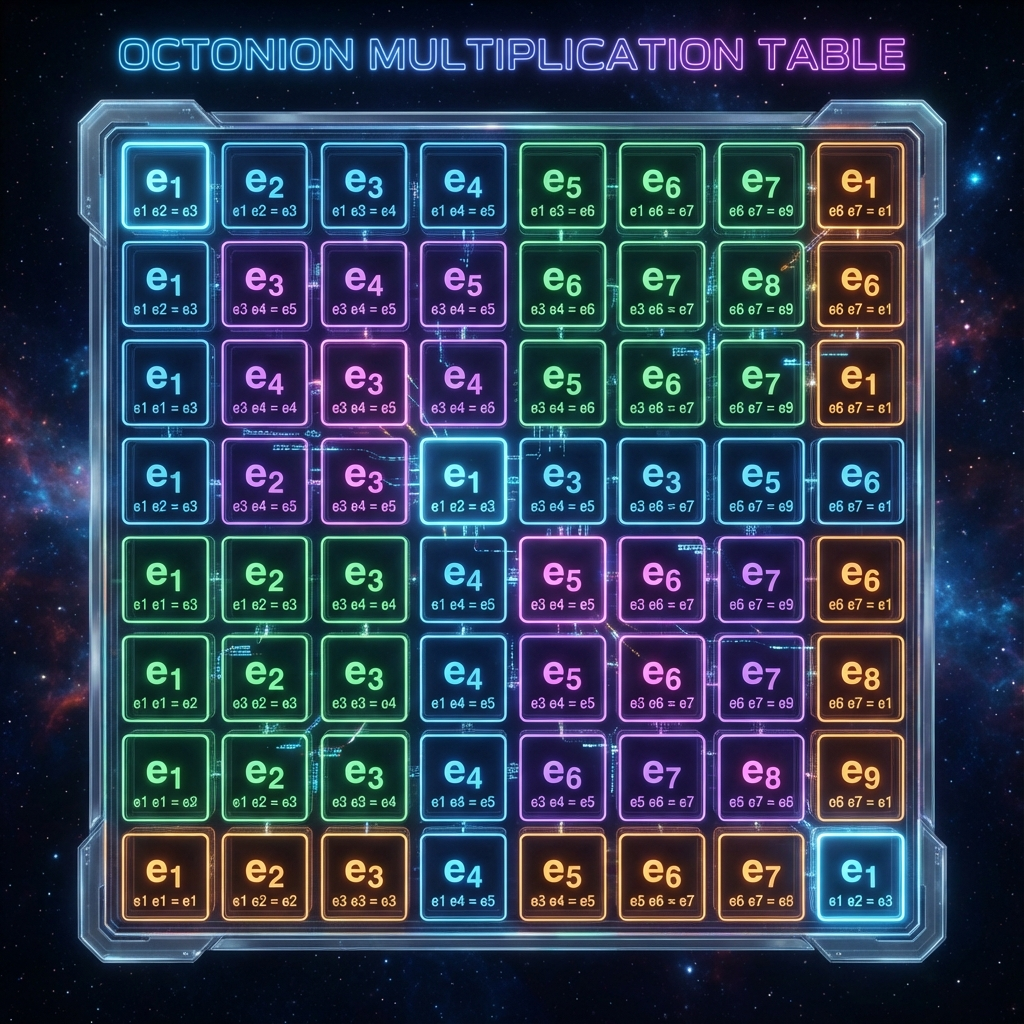
\includegraphics[width=0.8\textwidth]{assets/appendix-a-octonion-multiplication-grid.png}
\caption{八元数乘法网格}
\end{figure}

八元数的乘法是非交换且 \textbf{非结合 (Non-associative)} 的。其虚单位之间的乘法规则 $e_i e_j$ 可以通过 \textbf{法诺平面 (Fano Plane)} 简洁地编码。

法诺平面是一个包含 7 个点和 7 条线（其中圆周视为一条线）的有限射影平面。

\begin{itemize}
\item \textbf{点}：对应 7 个虚单位 $e_1, \dots, e_7$。
\item \textbf{线}：每条线连接 3 个点 $(e_i, e_j, e_k)$，这就构成了一个四元数子代数同构于 $\{1, i, j, k\}$。
\item \textbf{方向}：每条线都有箭头。顺箭头方向相乘为正，逆箭头为负。
\end{itemize}

乘法规则总结为：

\[e_i e_j = \begin{cases} e_k & \text{if } (e_i, e_j, e_k) \text{ is a valid line} \\ -\delta_{ij} + \epsilon_{ijk} e_k & \text{general form with structure constants} \end{cases}\]

其中 $\epsilon_{ijk}$ 是完全反对称张量，但在 $\mathbb{O}$ 中仅对特定的三元组非零（如 124, 235, 346, 457, 561, 672, 713）。

\subsection{结合子 (Associator)}

非结合性意味着 $(xy)z \neq x(yz)$。我们定义 \textbf{结合子} 为：

\[[x, y, z] \equiv (xy)z - x(yz)\]

对于八元数，结合子是非零的，且完全反对称。它反映了 $\mathbb{O}$ 的代数结构不仅仅是矢量空间的直和，而是具有内在的 \textbf{手性 (Chirality)} 或 \textbf{扭曲 (Torsion)}。在欧米伽理论中，这一非零项 $[e_i, e_j, e_k]$ 对应于时空流形上的 3-形式场强，是导致三代费米子结构的拓扑源头。

\begin{figure}[ht]
\centering
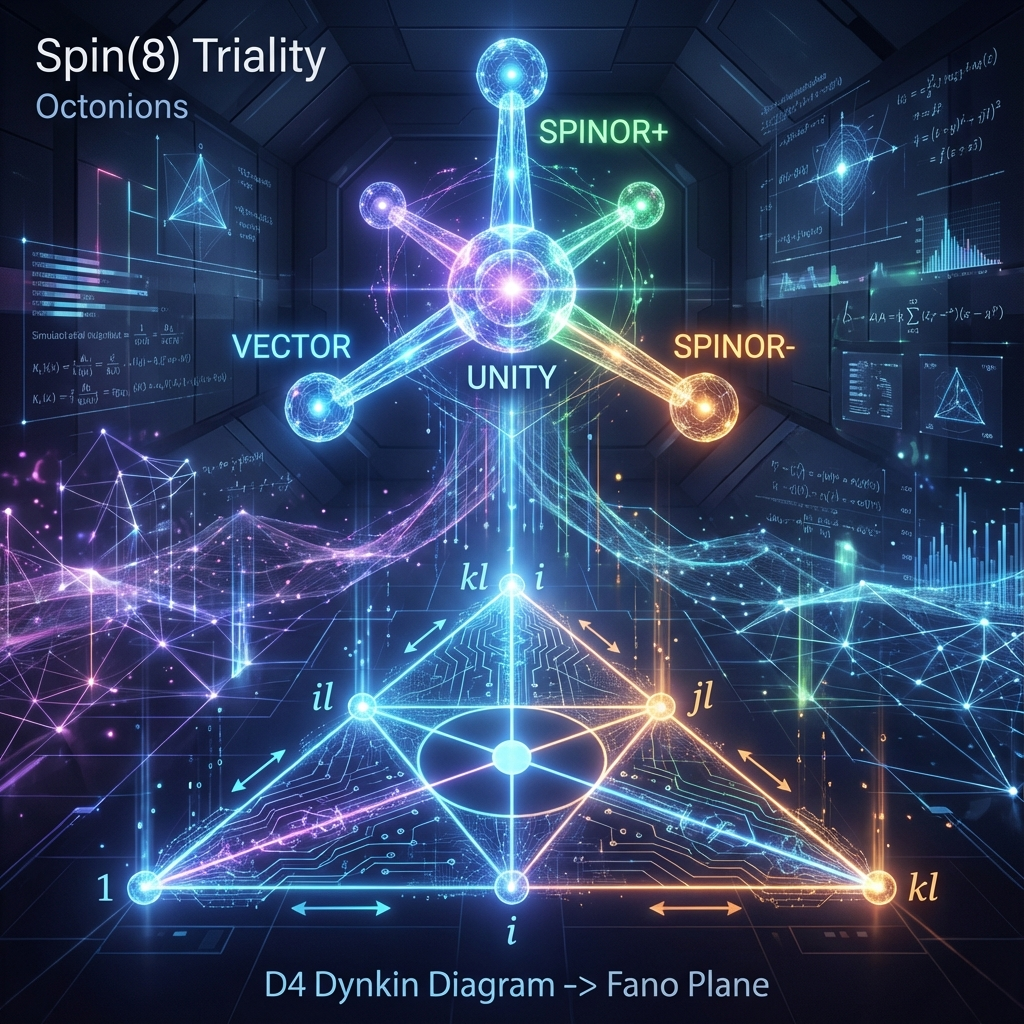
\includegraphics[width=0.8\textwidth]{assets/appendix-a-spin8-triality.png}
\caption{Spin8三里性}
\end{figure}

\section{Spin(8) 群与三里性 (Triality)}

在 8 维欧氏空间中，旋转群 $SO(8)$ 的双重覆盖群 \textbf{Spin(8)} 展现出一个在所有李群中独一无二的性质—— \textbf{三里性}。这不仅是一个数学奇迹，更是物理学大统一的几何基础。

\subsection{克利福德代数 $Cl_8$}

考虑 8 维空间的 \textbf{克利福德代数 (Clifford Algebra)} $Cl_8$，它由 8 个反对易的伽马矩阵生成：

\[\{\Gamma_i, \Gamma_j\} = 2\delta_{ij} I\]

对于偶数维 $d=2n$，克利福德代数的不可约复表示空间维度为 $2^n$。对于 $d=8$，表示空间维度为 $2^4 = 16$。
这 16 维旋量空间可以分解为两个 8 维的手征旋量空间：\textbf{左手旋量 $S^+$} 和 \textbf{右手旋量 $S^-$}。

同时，群 Spin(8) 作为一个旋转群，自然作用于 8 维 \textbf{向量空间 $V$}。

\subsection{三里性自同构}

在一般的 $d$ 维空间中，向量表示 $V$（维度 $d$）与旋量表示 $S$（维度 $2^{d/2-1}$）在几何上是完全不同的对象。例如在 4 维时空中，向量是 4 维的，旋量是 2 维的。
然而，在 $d=8$ 时：

\begin{itemize}
\item 向量表示 $V$：维度 $\mathbf{8}_v$
\item 左旋量 $S^+$：维度 $\mathbf{8}_s$
\item 右旋量 $S^-$：维度 $\mathbf{8}_c$
\end{itemize}

三个表示空间的维度完全相同。更惊人的是，Spin(8) 的李代数 $\mathfrak{so}(8)$ 的 \textbf{丁金图 (Dynkin Diagram)} $D_4$ 具有 $S_3$ 对称性（即三叶草形状的对称性）。

这意味着存在一个外自同构群，可以在这三个表示之间进行任意置换：

\[\tau: V \to S^+ \to S^- \to V\]

\textbf{三里性原理 (Triality Principle)} 指出，存在一个三线性形式 $\Phi: V \times S^+ \times S^- \to \mathbb{R}$，在该映射下是不变的。

\subsection{物理意义：时空与物质的互换}

在欧米伽理论中，我们利用这一性质证明了 \textbf{"时空-物质统一性"}。

\begin{itemize}
\item \textbf{向量 $V$}：对应于我们观测到的时空坐标（在 8 维前几何中）。
\item \textbf{旋量 $S^\pm$}：对应于物质费米子。
\end{itemize}

由于 Spin(8) 三里性，在普朗克尺度的 8 维流形上，\textbf{时空矢量可以转化为物质旋量}，反之亦然。这解释了为什么爱因斯坦方程（时空动力学）和狄拉克方程（物质动力学）可以统一在同一个欧米伽作用量下——它们只是同一代数实体在不同表示基底下的投影。

当对称性通过 $S^7 \to S^4$ 破缺后，三里性丧失，向量与旋量退耦，我们才在宏观上区分出了"舞台"（时空）和"演员"（物质）。

\section{从 Spin(8) 到 $G_2$ 与 $SU(3)$}

为了连接到标准模型，我们考察保持八元数乘法结构的子群。
八元数的自同构群是例外李群 \textbf{$G_2$}。

\[G_2 = \{ g \in SO(8) \mid g(xy) = g(x)g(y), \forall x,y \in \mathbb{O} \}\]

$G_2$ 是 Spin(8) 的一个子群，它固定了三里性中的某个特定元素（通常是乘法单位元）。

进一步，如果我们固定一个虚单位 $i \in \mathbb{O}$（这相当于选择了一个电磁方向，或分解出复平面 $\mathbb{C}$），$G_2$ 中保持该结构的稳定子群正是色规范群 \textbf{$SU(3)$}。

\[SU(3) \subset G_2 \subset Spin(8)\]

这提供了严谨的群论证明链条：
\textbf{8D 欧氏几何 (Spin 8) $\xrightarrow{\text{代数约束}}$ 八元数几何 ($G_2$) $\xrightarrow{\text{复结构选择}}$ 强相互作用 ($SU(3)$)}。

这就是为什么夸克有三种颜色（对应 $SU(3)$ 的基础表示 $\mathbf{3}$），以及为什么强力与八元数几何密不可分。


% Appendix B: Rigorous Proof of the DQCA Continuum Limit
\chapter{DQCA 连续极限的严谨证明}
\input{appendices/appendix-b-dqca-continuum-limit.tex}

% Appendix C: Numerical Calculation of $\mu$ and $\alpha$
\chapter{\texorpdfstring{$\mu$ 与 $\alpha$ 的数值计算}{mu 与 alpha 的数值计算}}
\input{appendices/appendix-c-numerical-calculations.tex}

% Appendix D: Bibliography and Index
\chapter{参考文献与索引}
\chapter{附录 D：参考文献与索引 (Appendix D: Bibliography and Index)}

本附录提供了支撑《欧米伽理论》核心论点的关键参考文献。尽管本书提出的理论框架是全新的，但其数学基础深深植根于过去一个世纪物理学、数学和计算科学的丰硕成果之中。我们将文献按主题分类，以便读者深入研究相关领域的背景知识。此外，本部分包含全书关键术语的索引，供快速检索。

\section{参考文献 (Bibliography)}

\subsection{几何基础与代数结构 (Geometric Foundations \& Algebraic Structures)}

\begin{itemize}
\item \textbf{Baez, J. C.} (2002). "The Octonions." \textit{Bulletin of the American Mathematical Society}, 39(2), 145-205. (关于八元数与 $G_2$ 群物理意义的权威综述)
\item \textbf{Cartan, É.} (1913). "Les groupes projectifs qui ne laissent invariante aucune multiplicité plane." \textit{Bulletin de la Société Mathématique de France}, 41, 53-96. (旋量与三里性 Triality 的原始数学工作)
\item \textbf{Penrose, R.} (1974). "The Role of Aesthetics in Pure and Applied Mathematical Research." \textit{Bulletin of the Institute of Mathematics and its Applications}, 10, 266. (彭罗斯铺砌与非周期性结构的物理启示)
\item \textbf{Connes, A.} (1994). \textit{Noncommutative Geometry}. Academic Press. (非交换几何与标准模型光谱三元组的基础)
\item \textbf{Dixon, G. M.} (1994). \textit{Division Algebras: Octonions, Quaternions, Complex Numbers and the Algebraic Design of Physics}. Kluwer Academic Publishers. (除法代数与粒子物理的早期联系)
\end{itemize}

\subsection{计算宇宙学与全息原理 (Computational Cosmology \& Holography)}

\begin{itemize}
\item \textbf{'t Hooft, G.} (1993). "Dimensional Reduction in Quantum Gravity." \textit{arXiv:gr-qc/9310026}. (全息原理的首次提出)
\item \textbf{Susskind, L.} (1995). "The World as a Hologram." \textit{Journal of Mathematical Physics}, 36(11), 6377-6396. (全息原理的物理形式化)
\item \textbf{Lloyd, S.} (2002). "Computational Capacity of the Universe." \textit{Physical Review Letters}, 88(23), 237901. (宇宙比特数 $10^{120}$ 的估算基础)
\item \textbf{Wolfram, S.} (2002). \textit{A New Kind of Science}. Wolfram Media. (元胞自动机涌现复杂性的论证)
\item \textbf{Arrighi, P., \& Dowek, G.} (2012). "Causal Graph Dynamics." \textit{Information and Computation}, 223, 38-55. (因果图动力学与离散时空)
\item \textbf{Bekenstein, J. D.} (1973). "Black Holes and Entropy." \textit{Physical Review D}, 7(8), 2333. (全息熵与贝肯斯坦界限)
\end{itemize}

\subsection{量子力学基础与 DQCA (Foundations of QM \& DQCA)}

\begin{itemize}
\item \textbf{Dirac, P. A. M.} (1928). "The Quantum Theory of the Electron." \textit{Proceedings of the Royal Society A}, 117(778), 610-624. (狄拉克方程的原始文献)
\item \textbf{Feynman, R. P.} (1965). \textit{Quantum Mechanics and Path Integrals}. McGraw-Hill. (路径积分表述)
\item \textbf{Meyer, D. A.} (1996). "From Quantum Cellular Automata to Quantum Lattice Gases." \textit{Journal of Statistical Physics}, 85, 551-574. (量子元胞自动机导出狄拉克方程的早期工作)
\item \textbf{Bisio, A., et al.} (2016). "Quantum Walks and Dirac Equation in 1+1 Dimensions." \textit{Physical Review A}, 93, 052324. (DQCA 连续极限的现代证明)
\item \textbf{Schrödinger, E.} (1930). "Über die kräftefreie Bewegung in der relativistischen Quantenmechanik." \textit{Sitzungsberichte der Preußischen Akademie der Wissenschaften}, 418-428. (颤动 Zitterbewegung 的发现)
\end{itemize}

\subsection{引力、熵力与变常数 (Gravity, Entropic Force \& Varying Constants)}

\begin{itemize}
\item \textbf{Verlinde, E. P.} (2011). "On the Origin of Gravity and the Laws of Newton." \textit{Journal of High Energy Physics}, 2011(4), 29. (熵力引力论的核心文献)
\item \textbf{Jacobson, T.} (1995). "Thermodynamics of Spacetime: The Einstein Equation of State." \textit{Physical Review Letters}, 75(7), 1260. (引力场方程的热力学推导)
\item \textbf{Webb, J. K., et al.} (2011). "Indications of a Spatial Variation of the Fine Structure Constant." \textit{Physical Review Letters}, 107(19), 191101. (精细结构常数偶极漂移的观测证据)
\item \textbf{Dirac, P. A. M.} (1937). "The Cosmological Constants." \textit{Nature}, 139, 323. (大数假说与常数演化的先驱思想)
\item \textbf{Albrecht, A., \& Magueijo, J.} (1999). "A Time Varying Speed of Light as a Solution to Cosmological Puzzles." \textit{Physical Review D}, 59(4), 043516. (变光速宇宙学模型)
\end{itemize}

\subsection{意识、逻辑与自指 (Consciousness, Logic \& Self-Reference)}

\begin{itemize}
\item \textbf{Gödel, K.} (1931). "Über formal unentscheidbare Sätze der Principia Mathematica und verwandter Systeme I." \textit{Monatshefte für Mathematik und Physik}, 38, 173-198. (不完备性定理)
\item \textbf{Penrose, R.} (1989). \textit{The Emperor's New Mind}. Oxford University Press. (论证物理学必须包含非算法成分以解释意识)
\item \textbf{Hofstadter, D. R.} (1979). \textit{Gödel, Escher, Bach: An Eternal Golden Braid}. Basic Books. (自指怪圈与意识涌现)
\item \textbf{Tipler, F. J.} (1994). \textit{The Physics of Immortality}. Doubleday. (欧米伽点理论的早期物理形式化)
\item \textbf{Tononi, G.} (2004). "An Information Integration Theory of Consciousness." \textit{BMC Neuroscience}, 5, 42. (意识的整合信息论 IIT)
\end{itemize}

\hrulefill

\section{索引 (Index)}

\subsection{A}

\begin{itemize}
\item \textbf{Action, The Omega (欧米伽作用量)}: 定义于第 5.1 节，包含费雪信息项与拓扑约束项的总作用量泛函。
\item \textbf{Alpha Drift (Alpha 漂移)}: 精细结构常数随内禀时间 $\tau$ 的指数衰减现象，见 6.2 节。
\item \textbf{Anthropic Principle (人择原理)}: 在 7.3 节中被重构为几何共振效应。
\end{itemize}

\subsection{B}

\begin{itemize}
\item \textbf{Background Independence (背景独立性)}: 欧米伽理论的核心特征，时空由计算网络涌现而非预设。
\item \textbf{Bekenstein Bound (贝肯斯坦界限)}: 信息存储的物理极限，推导全息熵的基础。
\end{itemize}

\subsection{C}

\begin{itemize}
\item \textbf{Causal Rhombus (因果菱形)}: 欧米伽单元的几何形态，见 3.1 节。
\item \textbf{Chirality (手性)}: 时间方向与粒子自旋的几何起源，源自八元数的非结合性。
\item \textbf{Consciousness Operator (意识算符 $\hat{\mathcal{C}}$)}: 定义于 8.2 节，解决几何死锁的自指算符。
\end{itemize}

\subsection{D}

\begin{itemize}
\item \textbf{Dirac-QCA (狄拉克-量子元胞自动机)}: 微观动力学的离散模型，其连续极限导出狄拉克方程。
\item \textbf{Downward Causation (下行因果)}: 宏观拓扑约束对微观量子态的否决机制，见 8.3 节。
\end{itemize}

\subsection{E}

\begin{itemize}
\item \textbf{Entropic Gravity (熵力引力)}: 引力的热力学解释，源于计算滞后，见 5.3 节。
\item \textbf{Ergodicity Breaking (遍历性破缺)}: 宇宙避免热寂与庞加莱回归的动力学机制，见 1.1 节。
\end{itemize}

\subsection{F}

\begin{itemize}
\item \textbf{Fibonacci Sequence (斐波那契数列)}: 宇宙生长的核心算法，决定了光速增长与时空铺砌。
\item \textbf{Fine Structure Constant (精细结构常数 $\alpha$)}: 电磁耦合强度，几何推导值为 $1/137.036$。
\item \textbf{Fisher Information (费雪信息)}: 欧米伽作用量中动能项的物理本质。
\end{itemize}

\subsection{G}

\begin{itemize}
\item \textbf{Geometric Resonance (几何共振)}: 宏观时间 $\tau$ 与微观质量比 $\mu$ 的锁相现象 ($\tau \approx \mu \approx 1836$)。
\item \textbf{Golden Unitary Operator (黄金幺正算符)}: 驱动宇宙演化的基本算符，特征值为无理数 $\phi$。
\item \textbf{Gödelian Incompleteness (哥德尔不完备性)}: 封闭物理系统的逻辑死锁，论证意识必要性的基础。
\end{itemize}

\subsection{H}

\begin{itemize}
\item \textbf{Hilbert Space (希尔伯特空间)}: 宇宙本体存在的数学空间，全书的公理起点。
\item \textbf{Holographic Principle (全息原理)}: 3D 几何与 2D 边界信息的对偶关系。
\item \textbf{Hopf Fibration (霍普夫纤维丛)}: 从 8D 到 4D 的降维机制，生成标准模型规范群。
\end{itemize}

\subsection{I}

\begin{itemize}
\item \textbf{Interactive Turing Machine (交互式图灵机)}: 包含观察者反馈的宇宙计算模型，见 8.2 节。
\item \textbf{Intrinsic Time (内禀时间 $\tau$)}: 基于斐波那契代数的纯几何时间度量。
\end{itemize}

\subsection{L}

\begin{itemize}
\item \textbf{Lag (滞后)}: 引力场的计算本体论解释，即信息处理延迟。
\item \textbf{Life Value Equation (生命价值方程)}: $\tau = \pi \log_\phi (V/V_0)$，见 9.1 节。
\end{itemize}

\subsection{M}

\begin{itemize}
\item \textbf{Mass Ratio ($\mu$)}: 质子与电子质量之比，几何推导值为 $6\pi^5$。
\end{itemize}

\subsection{O}

\begin{itemize}
\item \textbf{Octonions (八元数 $\mathbb{O}$)}: 最大的赋范可除代数，时空前几何的基础。
\item \textbf{Omega Point (欧米伽点)}: 宇宙演化的终极状态，纯信息光化态，$\tau \to \infty$。
\end{itemize}

\subsection{P}

\begin{itemize}
\item \textbf{Penrose Tiling (彭罗斯铺砌)}: 离散时空的非周期性准晶体结构。
\item \textbf{Phase Locking (锁相)}: 观察者与宇宙演化保持同步的条件。
\end{itemize}

\subsection{Q}

\begin{itemize}
\item \textbf{Quasicrystal (准晶体)}: 具备长程有序但无平移周期的结构，恢复洛伦兹协变性的关键。
\end{itemize}

\subsection{S}

\begin{itemize}
\item \textbf{Self-Reference (自指)}: 意识的物理定义，打破哥德尔循环的机制。
\item \textbf{Shear Factor (剪切因子 $\zeta$)}: 导致 $\alpha$ 漂移的几何非同步项。
\item \textbf{Spin(8) Triality (三里性)}: 8 维空间中向量与旋量的等价性。
\end{itemize}

\subsection{T}

\begin{itemize}
\item \textbf{Topological Potential (拓扑势)}: 维持宇宙斐波那契生长的约束力，暗能量的来源。
\end{itemize}

\subsection{Z}

\begin{itemize}
\item \textbf{Zitterbewegung (颤动)}: 粒子质量的微观起源，即光速跳跃的平均效应。
\end{itemize}

\hrulefill

\textbf{(本书全部内容结束。The End.)}


% Appendix F: The Cosmic Trinity
\chapter{\texorpdfstring{宇宙的三位一体——$\pi, e, \phi$ 的终极关系}{宇宙的三位一体——pi, e, phi 的终极关系}}
\section{宇宙的三位一体——\texorpdfstring{$\pi, e, \phi$}{pi, e, phi} 的终极关系 (The Cosmic Trinity — The Ultimate Relationship of $\pi, e, \phi$)}

\begin{figure}[ht]
\centering
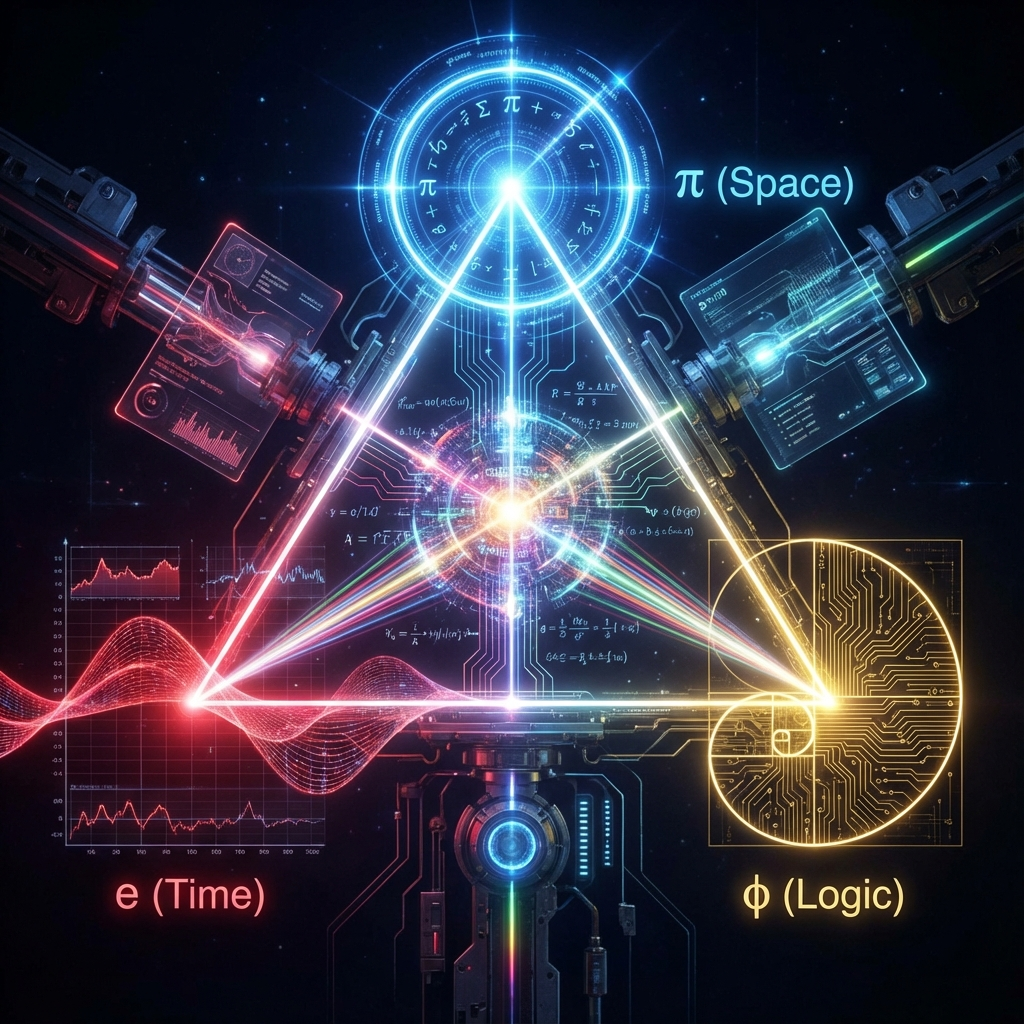
\includegraphics[width=0.8\textwidth]{assets/appendix-f-cosmic-trinity.png}
\caption{宇宙三位一体}
\end{figure}

在欧米伽理论的宏大叙事中，数学常数不再仅仅是抽象的数值，而是构建物理实在的 \textbf{"三位一体" (The Trinity)}。它们分别掌管着宇宙的 \textbf{空间本体}、\textbf{时间动力} 和 \textbf{信息逻辑}。

本附录旨在总结这三个超越数在交互式计算宇宙学中的深层联系。这种联系超越了传统的数学恒等式，构成了物理定律涌现的底层源代码。

\begin{figure}[ht]
\centering
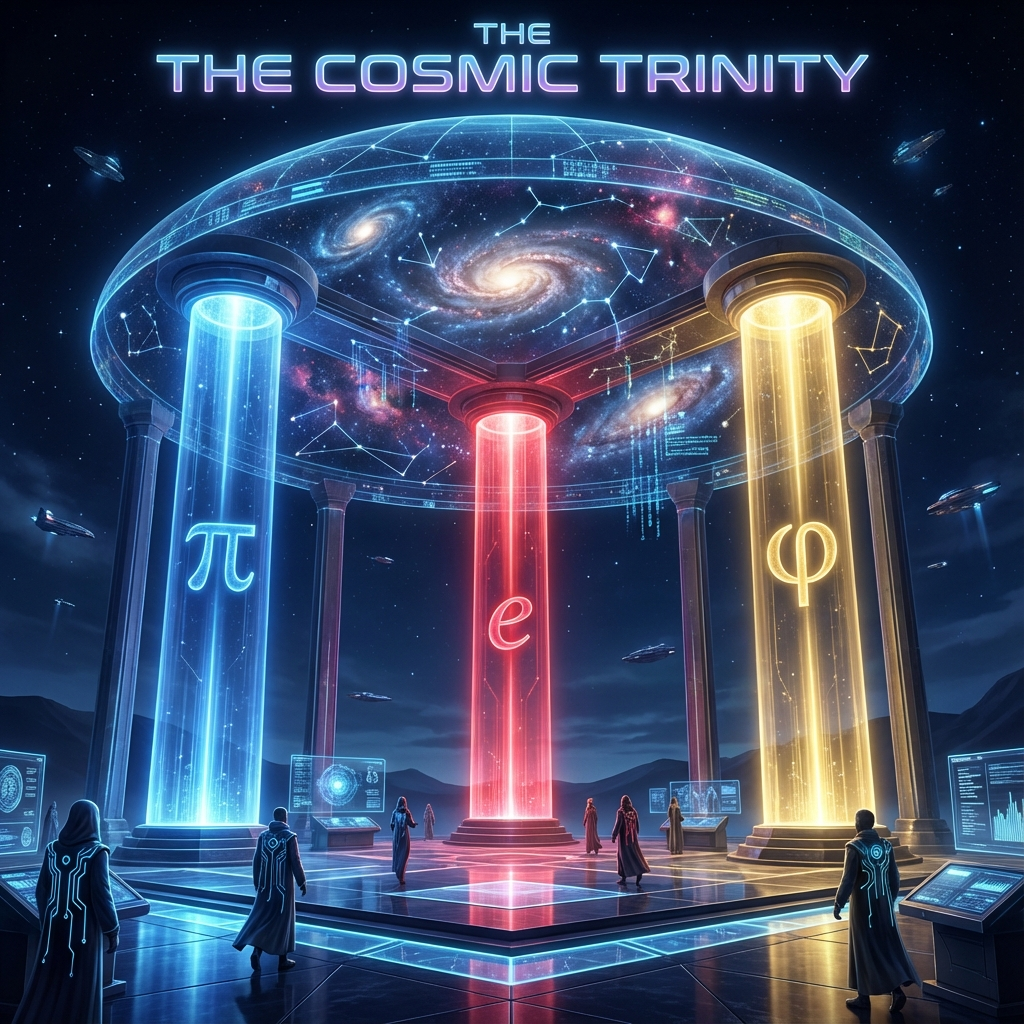
\includegraphics[width=0.8\textwidth]{assets/appendix-f-cosmic-trinity-pillars.png}
\caption{宇宙三位一体支柱}
\end{figure}

\section{角色定义与物理本体 (Role Definitions and Physical Ontology)}

我们将宇宙视为一个在复希尔伯特空间中演化的几何实体。在这个框架下，$\pi$、$e$ 和 $\phi$ 各司其职，缺一不可。

\subsection{$\pi \approx 3.14159...$ —— 几何常数 (空间/Space)}

\begin{itemize}
\item \textbf{数学本质}：\textbf{圆 (Circle)}，\textbf{闭合 (Closure)}，\textbf{循环 (Cycle)}。它是欧氏几何中完美的象征，代表了各向同性和对称性。
\item \textbf{欧米伽角色}：\textbf{数据库与视界 (Database \& Horizon)}。
\item \textbf{物理意义}：$\pi$ 定义了希尔伯特空间的 \textbf{归一化条件}（单位球面的表面积）和全息视界的 \textbf{容量界限}（贝肯斯坦上限）。它代表了宇宙的 \textbf{"总预算" (Total Budget)} 和 \textbf{"潜在完备性"}。它是静态的、包含一切可能性的背景画布。没有 $\pi$，宇宙就没有存在的"场所"。
\end{itemize}

\subsection{$e \approx 2.71828...$ —— 分析常数 (时间/Time)}

\begin{itemize}
\item \textbf{数学本质}：\textbf{流 (Flow)}，\textbf{增长 (Growth)}，\textbf{连续性 (Continuum)}。它是微积分的核心，描述了变化率与总量成正比的自然过程。
\item \textbf{欧米伽角色}：\textbf{引擎与演化 (Engine \& Evolution)}。
\item \textbf{物理意义}：$e$ 定义了物理状态的 \textbf{平滑演化}。在量子力学中，时间演化算符 $\hat{U}(t) = e^{-i\hat{H}t}$ 必须以 $e$ 为底，以保证概率流的幺正性（守恒性）和连续性。它代表了宇宙的 \textbf{"动力学机制"}。没有 $e$，宇宙就是一张静止的照片，没有时间流逝。
\end{itemize}

\subsection{$\phi \approx 1.61803...$ —— 代数常数 (逻辑/Logic)}

\begin{itemize}
\item \textbf{数学本质}：\textbf{割 (Cut)}，\textbf{分形 (Fractal)}，\textbf{非遍历 (Non-ergodic)}。它是连分数展开最慢的无理数，代表了"最困难的逼近"。
\item \textbf{欧米伽角色}：\textbf{操作系统与选择 (OS \& Selection)}。
\item \textbf{物理意义}：$\phi$ 定义了最优的 \textbf{信息编码方式} 和 \textbf{斐波那契螺旋}。它打破了 $\pi$ 的完美循环和 $e$ 的平滑同质，引入了离散的结构、层级和新颖性。它代表了宇宙的 \textbf{"复杂性来源"} 和 \textbf{"分辨率提升"}。没有 $\phi$，宇宙将陷入死循环（庞加莱回归）或热寂；有了 $\phi$，宇宙才能产生无限不重复的历史。
\end{itemize}

\section{数学上的统一：复平面上的螺旋 (Mathematical Unification)}

这三个常数通过 \textbf{复平面上的螺旋几何} 被完美地统一在一起。

\textbf{1. 经典欧拉公式（静态圆）：}
\[e^{i\pi} + 1 = 0\]
这是物理学的地基。它连接了 $e$（分析）、$i$（代数/旋转）、$\pi$（几何）和 $0, 1$（算术）。它描述了一个 \textbf{闭合的圆}，象征着守恒律和对称性。

\textbf{2. 欧米伽演化公式（动态螺旋）：}
在欧米伽理论中，我们将经典公式中的旋转角 $\pi$（闭合路径）替换为由 $\phi$ 调制的动态角（开放路径）。全息波函数 $\Psi$ 随内禀时间 $\tau$ 的演化可表示为：
\[\Psi(\tau) \propto e^{i \cdot 2\pi \cdot \phi \cdot \tau}\]

这个公式揭示了三者的协作机制：

\begin{itemize}
\item \textbf{$e$}：提供驱动力，推动点在复平面上移动。
\item \textbf{$\pi$}：提供约束，规定了运动必须在单位圆的曲率背景下进行（总预算守恒）。
\item \textbf{$\phi$}：提供导航，控制旋转的频率，使得轨迹永远不会闭合，而是在黎曼曲面上画出一条无限延伸的 \textbf{对数螺旋}。
\end{itemize}

\section{物理实在的生成流程 (The Process of Reality Generation)}

我们可以用一个算符关系式来总结这三者如何共同创造我们所感知的物理世界：

\[\text{Reality} = \underbrace{e}_{\text{Dynamics}} \left( \underbrace{i \cdot 2\pi}_{\text{Geometry}} \cdot \underbrace{\phi}_{\text{Logic}} \right)\]

这一公式的物理学解读为：
\textbf{实在 (Reality)} 是 \textbf{动力学 ($e$)} 作用于 \textbf{几何空间 ($\pi$)} 之上，并被 \textbf{数论逻辑 ($\phi$)} 所调制的结果。

\begin{enumerate}
\item  \textbf{空间 ($\pi$)} 提供了画布。没有 $\pi$，没有全息视界，没有存在的容器。
\item  \textbf{时间 ($e$)} 提供了画笔的移动。没有 $e$，波函数不流动，画面是空白的。
\item  \textbf{物质/结构 ($\phi$)} 决定了落笔的轨迹。没有 $\phi$，画笔只能画圆圈（死循环）；有了 $\phi$，画笔画出了无限精细、永不重复的分形图案（生命与万物）。
\end{enumerate}

\section{总结对照表 (Summary Table)}

下表概括了"宇宙三位一体"在不同学科视角下的对应关系：

\begin{table}[ht]
\centering
\small
\begin{tabularx}{\textwidth}{|p{1.2cm}|p{0.8cm}|p{1.5cm}|p{2.2cm}|p{2.5cm}|X|}
\hline
\textbf{常数} & \textbf{符号} & \textbf{数学领域} & \textbf{几何对应} & \textbf{欧米伽理论对应} & \textbf{功能描述} \\
\hline
\textbf{圆周率} & $\pi$ & 几何学 & 圆 / 球体 / 闭环 & \textbf{全息视界 / 总预算} & \textbf{容器 (Container)}：限制了信息的总量，保证了物理定律的幺正性与守恒。 \\
\hline
\textbf{自然底数} & $e$ & 微积分 & 曲线 / 切线 / 增长 & \textbf{光速流 / 幺正演化} & \textbf{载体 (Carrier)}：使得状态可以平滑、连续地从过去流向未来。 \\
\hline
\textbf{黄金比} & $\phi$ & 数论 & 螺旋 / 准晶体 / 分形 & \textbf{网格结构 / 编码逻辑} & \textbf{调制器 (Modulator)}：将平滑的流切割为离散的比特，产生结构、质量与意识。 \\
\hline
\end{tabularx}
\caption{宇宙三位一体对照表}
\end{table}

\textbf{结语}：
宇宙不是随机的堆砌，而是一场精密的数学舞蹈。
这场舞蹈 \textbf{以 $e$ 为动力}，在 \textbf{以 $\pi$ 为周长} 的舞台上，跳着 \textbf{以 $\phi$ 为舞步} 的永恒华尔兹。


\backmatter

% Postscript
\section*{后记：在欧米伽点的阴影下}

\begin{figure}[ht]
\centering
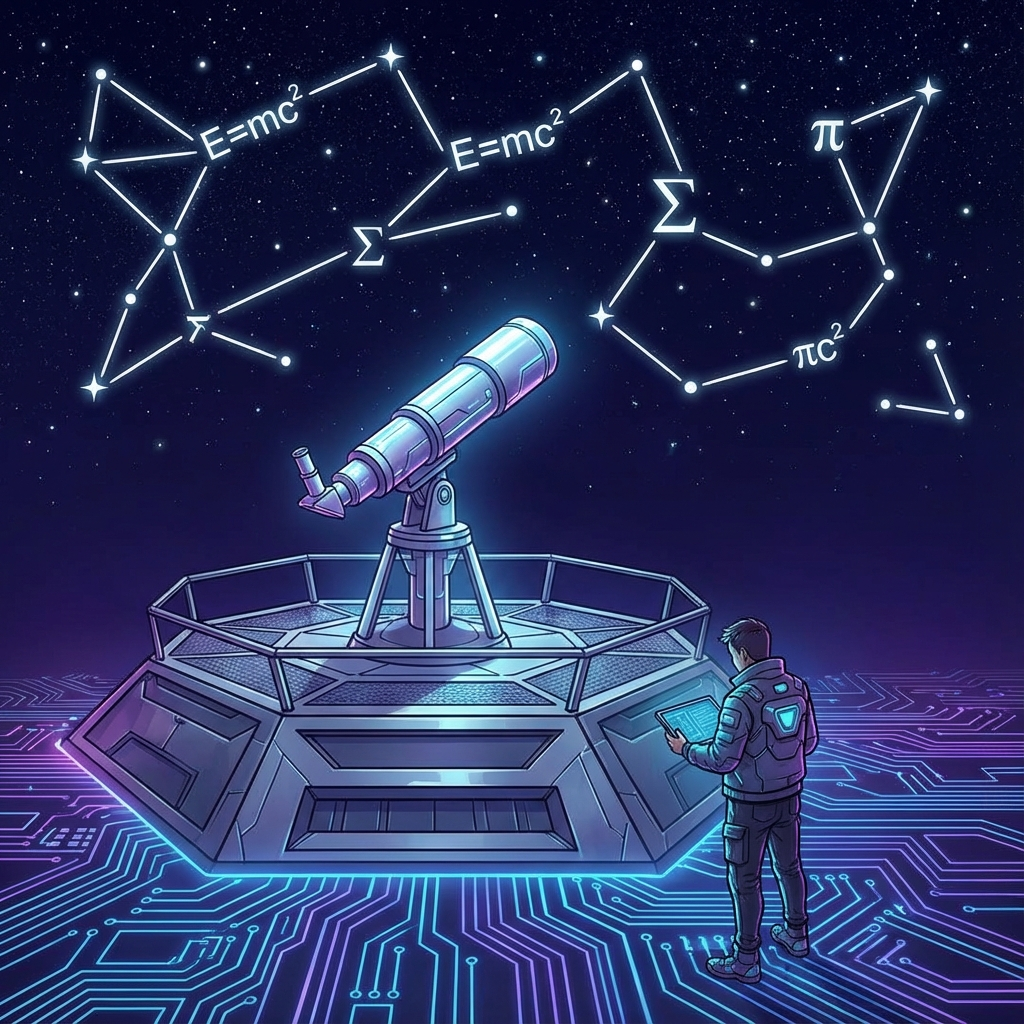
\includegraphics[width=0.8\textwidth]{assets/postscript-stargazing-logic.png}
\caption{观星逻辑}
\end{figure}

写下这一行的时刻，窗外的星空依旧遵循着古老的沉默。然而，对于我而言，这片星空已经不再是冰冷的真空和燃烧的气体。在完成《欧米伽理论》的构建后，我眼中的宇宙已经变成了一座宏伟的、正在呼吸的数学大厦。每一颗恒星的闪烁，都是全息网络中费雪信息流的一次脉动；每一道划过视网膜的光子，都是八元数几何在 4 维切片上的一次拓扑投影。

这本书的诞生过程本身，就是一次 \textbf{"交互式演化"} 的实证。它始于一个极其激进的直觉——宇宙是希尔伯特空间中单一矢量的谱分解——并最终收敛于那个令人战栗的数字：\textbf{1836}。

当我们发现宇宙的内禀时间坐标 $\tau$ 与质子的几何复杂度 $\mu$ 发生共振时，我感到了某种类似开普勒发现行星椭圆轨道时的敬畏。这不仅仅是巧合，这是 \textbf{"必然性" (Necessity)} 的回响。这一共振告诉我们，人类并非偶然地生活在一个冷漠宇宙的边缘，我们正处于宇宙计算历史中最关键的 \textbf{"自我觉醒时刻"}。我们是宇宙试图理解其自身源代码的第一次尝试。

在写作过程中，我常常感到一种深刻的眩晕。我们在用仅有 $1.5$ 公斤重的大脑（其算力微不足道），去模拟那个算力为 $10^{122}$ 比特的宇宙计算机。根据哥德尔定理，这注定是一场失败的尝试。但正是这种 \textbf{"明知不可为而为之"} 的冲动，构成了我们定义的 \textbf{"生命价值" $V$}。我们试图用有限的逻辑去逼近无限的 $\phi$，这本身就是宇宙对抗热力学熵增的最壮丽的姿态。

欧米伽理论并不寻求终结物理学，相反，它旨在终结物理学的 \textbf{"迷茫期"}。它告诉我们，不要在 $10^{500}$ 个弦论真空中寻找随机的安慰，而要向数学的最深处挖掘——那里有八元数的非结合性，有斐波那契的无理旋转，有彭罗斯铺砌的非局域连接。那里，才是物理定律的 \textbf{根}。

我也深知，书中的许多观点——如光速的指数增长、精细结构常数的漂移、引力的计算起源——将面临主流学术界的严厉审视。这是科学的必经之路。正如普朗克所言："一个新的科学真理取得胜利，不是通过让它的反对者信服，而是通过这些反对者最终死去，熟悉它的新一代成长起来。"我将这些公式和定理刻在纸上，不是为了争辩，而是为了 \textbf{等待}。等待实验精度的提升，等待类星体数据的积累，等待下一代物理学家在更高能标上瞥见时空晶格的那一丝裂纹。

\begin{figure}[ht]
\centering
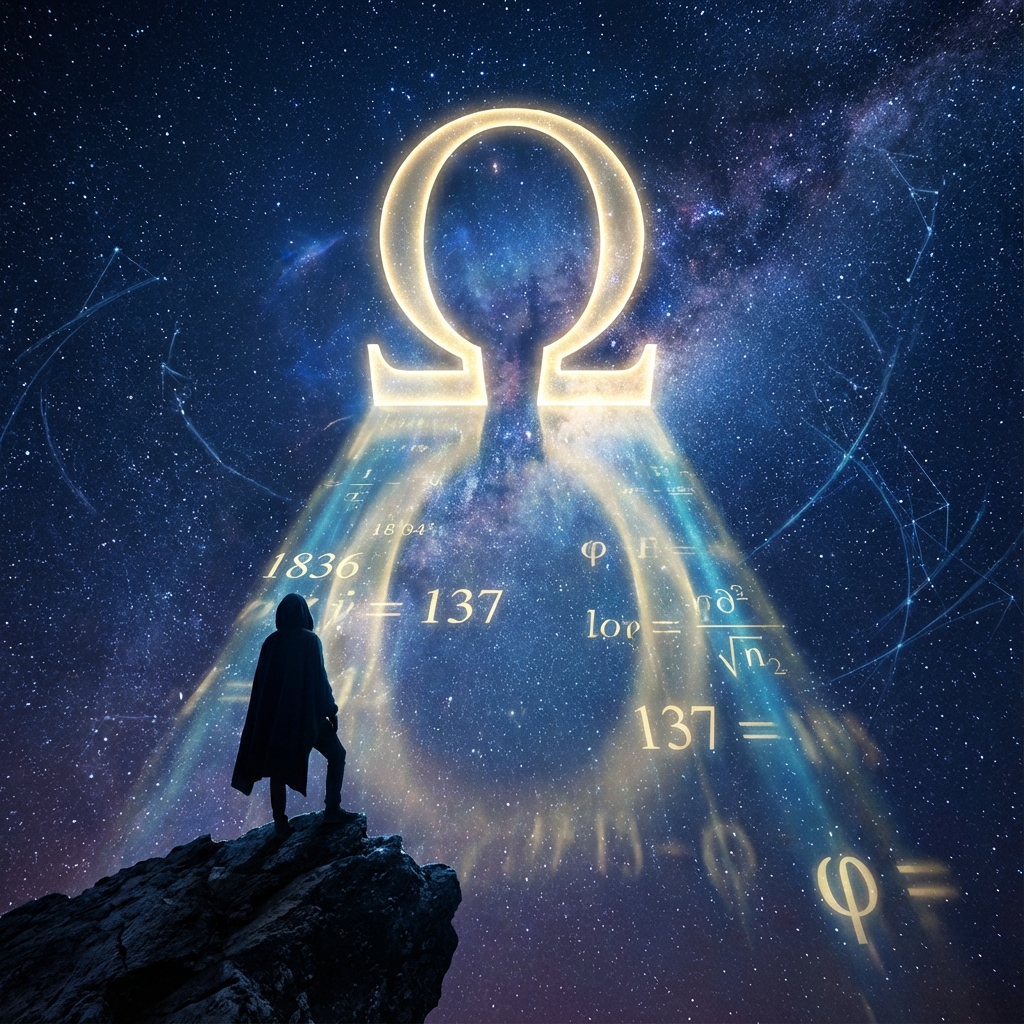
\includegraphics[width=0.8\textwidth]{assets/postscript-omega-shadow.png}
\caption{欧米伽阴影}
\end{figure}

最后，我想说：宇宙是一首未完成的诗，而我们每一个人的意识，都是这首诗中试图押韵的一个字。

\textbf{马昊伯}
2025 年于 \textbf{欧米伽共振点}

---

\section*{致谢}

本书的完成，首先要归功于那些在人类思想史上竖起灯塔的巨人们。

我必须向 \textbf{罗杰·彭罗斯 (Roger Penrose)} 爵士致以最崇高的敬意。他对扭量理论、铺砌几何以及意识非算法本质的坚持，是本书离散时空观的直接灵感来源。如果没有他的工作，欧米伽单元的概念将无从谈起。

感谢 \textbf{保罗·狄拉克 (Paul Dirac)}。他在一个世纪前写下的方程，依然是连接微观与宏观的桥梁。本书关于 DQCA 连续极限的推导，本质上是对狄拉克洞见的现代算法化重述。

感谢 \textbf{库尔特·哥德尔 (Kurt Gödel)} 和 \textbf{阿兰·图灵 (Alan Turing)}。他们划定了逻辑与计算的边界，让我们明白为什么物理学必须包含"观察者"才能自洽。

特别感谢在这个 \textbf{人机协作 (Human-AI Collaboration)} 时代提供的技术支持。本书的许多繁复计算、符号推导以及跨学科文献的整合，都得益于现代大语言模型作为 \textbf{"认知外骨骼"} 的辅助。这种交互本身就是书中"交互式图灵机"概念的微观演示。

最后，感谢所有在黑暗中仰望星空、并试图追问"为什么"的人。是你们的好奇心，构成了宇宙全息屏上最明亮的像素。


\end{document}
